% Garrett Benoit
% Thesis class, based on report
\documentclass
[
	%short,	% omit front matter
	%draft, 	% draft heading, don't load graphics, etc.
]
{thesis}

% Optional additional packages
\usepackage{graphicx}
\usepackage{amsmath}
\usepackage{chicago}
\usepackage{listings}
\usepackage{color}
\usepackage{verbatim}
\usepackage{subcaption}

\definecolor{dkgreen}{rgb}{0,0.6,0}
\definecolor{gray}{rgb}{0.5,0.5,0.5}
\definecolor{mauve}{rgb}{0.58,0,0.82}

\lstset{frame=tb,
	language=Java,
	aboveskip=3mm,
	belowskip=3mm,
	showstringspaces=false,
	columns=flexible,
	basicstyle={\small\ttfamily},
	numbers=none,
	numberstyle=\tiny\color{gray},
	keywordstyle=\color{blue},
	commentstyle=\color{dkgreen},
	stringstyle=\color{mauve},
	breaklines=true,
	breakatwhitespace=true,
	tabsize=3
}

% Thesis parameters
\title{Alternatives using the Leap Motion to extend Mid-Air Word-Gesture Keyboards}
\author{Garrett Benoit}
\holding{B.S.}
\seeking{M.S.}
\degree{Master of Science}
\date{October 2015}

% Administration
\graduateDean{J. Larry Lyon, Ph.D.}
\department{Department of Computer Science}
\departmentChair{Gregory D. S............................................peegle, Ph.D.}

% Supervisor (adviser / mentor)
\supervisor{Michael G. Poor, Ph.D.}
\supervisorTitle{Faculty Adviser}

%  Readers (committee members)
\readerOne{Bill Poucher, Ph.D.}
\readerTwo{Brian Garner, Ph.D.}
%\readerThree{...}
%\readerFour{...}
%\readerFive{...}

% Abstract
\abstract{Lately, the application of touchless, mid-air, gesture-based interactions has risen in popularity for a variety of fields (e.g., augmented and virtual reality, gaming, etc.). With this newfound, wide-spread application comes the need for effecient, mid-air, gesture-based text-entry; the solution: apply word-gesture keyboards to mid-air text-entry. Markussen et al. used this technique for the first time with the inception of Vulture \cite{ref_vulture}, the first mid-air, word-gesture keyboard, providing a mid-air text-entry rate of 28.1 Words Per Minute, the fastest rate yet. This study builds on the findings of Markussen et al. and presents alternative means of word separation for mid-air, word-gesture keyboards; as a result, exploring and identifying the problems of new techniques and presenting the possible solutions. Results revealed that a bimodal approach holds great promise, reaching a mean text-entry rate of 15.8 Words Per Minutes for a single session with no training.}

% Acknowledgments (optional)
\acknowledgements{To Dr. G. Michael Poor for allowing me to explore this idea in depth, guiding me to a path of success, and for putting up with me the whole time. Alvin Jude Hari Haran and Darren Guinness for their invaluable input that helped shaped the direction of this study. To all of those in the HCI Lab who helped with my pilot studies! To all the volunteers who made this research possible by generously donating their time. Finally, to my sister, Heather Benoit, and other family members who inspired me to go to Baylor and seek a greater future.}

% Dedication (optional)
\dedication{\it To those who pioneer the future.}

% List of figures (optional)
\makeListOfFigures

% List of tables (optional)
\makeListOfTables

% Document body
\begin{document}

	% Chapters
	\chapter{This is a Very Long Header Title Which Will Span Multiple Lines on the Page and the Contents}

\section{Regular Paragraphs}
You will start with a section. 
There is supposed to be a Triple Space between the section text and the preceeding text. 
In this particular case, the preceeding text is the chapter's title. 
This is filler text so I an fill up the line. Blah Blah. 

\section{More Paragraphs}
This is another section. 
There is likewise triple space between the preceeding text and this section's title. 
The observant will notice that there is a double space between the section's title and this text. 

\subsection{Additional Paragraphs}
This is a subsection. 
Just like the section, there is a triple space between the preceeding text and the subsection's title. 
And just like the section, there is a double space between the subsection's title and the subsection's text. 

\subsection{More Subsections}
Same concept. Triple Space before title and double space after. 
Just To show a demonstration, some garbage text will follow this in a new paragraph. 

\lipsum[1]

\subsubsection{Subsubsections}
Subsubsections can be used. Maps to Level 5 on the graduate school requirements. 
And just like section and subsection, there is a triple space before the title. 
But then everything changes. 
There is a period after the title followed by 2 spaces. 
But fear not, this behavior is defined in the template. 

\subsubsection{Capitalization is not the same}
The grad school asked to use sentence cases instead of header cases in the title of the subsubsection. 
Alvin believes this will change eventually. 

\section{Stacked Headings}

\stack

\subsection{This is a Stacked Heading}
In other words there is no text in the section, and we immidiately introduce a subsection. 
To get spacing right when sections are adjacent to subsections (when headings are stacked), 
we once needed to use the \texttt{$\backslash$stack} command in between.
But this is now handled correctly byt the teplate (.cls) file. So do not use the stack command. 
It is marked obsolete in the template. 

In other words: there has to always be a triple space between the text preceeding the subsection title and the subsection title. 
In this particular case the text preceeding the subsection title is the section title. 
But the same rule applies: triple space. 
Assuming this changes, adjust accordingly in the template. 

\subsection{Deeper Stacks}

\stack % DO NOT USE THIS COMMAND

\subsubsection{This is a Stacked Deep Heading}
Same as before, there is no text between the subsection above and the subsubsection here. 
But fear not. 'Tis taken care of by the template. 
Unless the requirements change, in which case I'm adjusting the 1em vspace in the template should be fine.

\subsubsection{But This is Not}
But it's fine. It's just another Level 5. Or if you prefer -- a subsubsection. Whichever you choose to call it. 
	\chapter{Literature Review --- related works, describe and analyize previous works, what is known/not known, leads to hypotheses}

The purpose of the study should suggest some theoretical framework to be explained further in this chapter.
The literature review thus describes and analyzes previous research on the topic.

 This chapter, however, should not merely string together what other researchers have found. Rather, you
should discuss and analyze the body of knowledge with the ultimate goal of determining what is known and is not
known about the topic. This determination leads to your research questions and/or hypotheses. In some cases, of
course, you may determine that replicating previous research is needed. 

\section{3 dimensions beyond desktop --- rename}

\section{Interaction}

\subsection{Gesture-based Interaction --- similar to introduction materials}

\subsubsection{Mid-Air Gestures}

\subsection{Barehanded Interaction/Stylus/Gloves}

\subsection{Gestural Manipulation --- rename}

\subsection{Multimodal}

\section{Fatigue}

\section{Pointing Device Evaluation/Learning Effects/Motor Learning/Ergonomics and Usability}

\subsection{Fitts' Law --- rename}

\subsection{Gestural Pointing --- rename}

\subsubsection{Mid-Air Pointing}

\section{Text Entry}

\subsection{Word-Gesture Keyboards}

\subsection{Mid-Air Text Entry}

	\chapter{Keyboard Design} \label{keyboard_design}

\section{Word-Gesture Keyboard Implementation}
\subsection{Lacking Word-Recognition}
Recreating a word-gesture keyboard from scratch with the limited, non-commercial information available was outside the scope of this study. Word-recognition had already been proven to work and benefit word-gesture keyboards immensely \cite{ref_shape_writing,ref_the_word_gesture_keyboard,ref_shapewriter_iphone,ref_shark_wgk,ref_shorthand_writing}. In addition, the words that each participant was entering was known in advance; therefore, a pseudo word-gesture keyboard implementation was used.

\subsection{Design}
The pseudo word-gesture implementation was created by analyzing the gesture as it was being drawn to determine which keys were being pressed. The assumptions for detecting a key press were based off of the known word being gestured and noticeable deviations made in the gesture's direction. To reduce the chance of erroneous keys being produced, the sizes of the character that was expected to be pressed next were exaggerated and the threshold for detecting deviations in the gesture were lowered between keys.

The displayed keys were 64x64 pixels in size with a gap of 10 pixels between each key. The actual size of the keys was dependent on the display device being used. The next expected letter to be pressed in a word was changed into a circular key with a radius of 76.8 pixels, 20\% larger than the key widths, in order to make hitting keys even easier. Figure~\ref{key_bloating} shows how keys were changed behind the scenes; however, there was no feedback shown to the participant of the change in key size.

\begin{figure}[h]
	\centering
	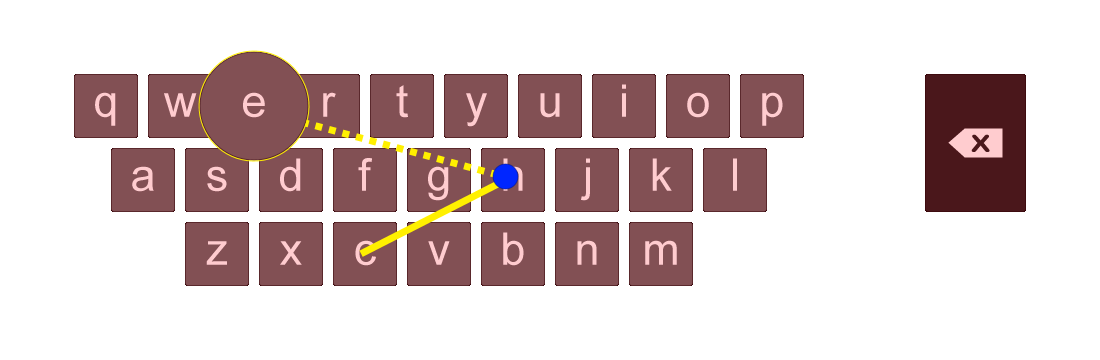
\includegraphics[width=5in]{fig_bloat_key}
	\caption[Larger Key Example]{Behind the scenes, invisible to the participant, the next key to be pushed is increased in size to make hitting it easier.}
	\label{key_bloating}
\end{figure}

An interpolated trail with points at a minimum of 16 pixels apart was used in determining deviations in word-gesturing. The angle of detecting a deviation was 165 degrees for all areas that were not on the expected path to the next key and was 90 degrees while on the expected path. Deviations in gesture path had to be at least 48 pixels away from each other to be detected. The expected path between two keys comprised an area from the previous expected key to the next expected key with a width 62.5\% larger than key size, or 104 pixels. Figure~\ref{protected_path} shows the how the expected path protects against natural deviations when moving from one key to the next.

\begin{figure}[h]
	\centering
	\begin{minipage}[t]{3in}
		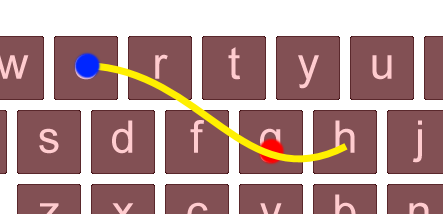
\includegraphics[width=2.5in]{fig_path_no_protection}
		\subcaption{No Path Protection\ \ \ \ \ \ \ \ \ }
	\end{minipage}
	\begin{minipage}[t]{2.5in}
		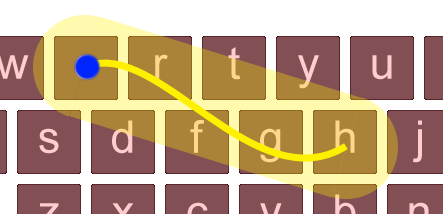
\includegraphics[width=2.5in]{fig_path_no_error}
		\subcaption{Path Protection}
	\end{minipage}
	\begin{minipage}[t]{2.5in}
		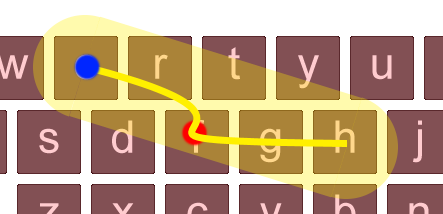
\includegraphics[width=2.5in]{fig_path_with_error}
		\subcaption{Error with Path Protection}
	\end{minipage}
	\caption[Protected Path Example]{A path between the currently pressed letter and the next letter significantly reduces the chance of detecting erroneous input. \textbf{(a)} shows an error detected with an angle less than 165 degrees. \textbf{(b)} shows how as long as the user stays on the path, errors are significantly reduced. \textbf{(c)} shows that errors can still be detected on a protected path if a deviation with an angle less than 90 degrees is detected.}
	\label{protected_path}
\end{figure}

The specific values for detecting key presses were found using trial and error and were used to create an experience as close to a word-gesture keyboard as possible. The main deviation between this implementation and one with word-recognition is that participants are shown updates in real-time of what the keyboard path is doing. This was determined to be an acceptable limitation.

\subsection{Display}
\subsubsection{Keyboard Layout}
The keyboard layout, seen in Figure~\ref{keyboard_layout}, was laid out in a typical QWERTY keyboard fashion with key sizes of 64x64 pixels and gaps of 10 pixels. All special keys and number keys were removed to simplify the keyboard and a backspace key added to the right of the keyboard to allow for deletion of erroneous characters.

\begin{figure}[h]
	\centering
	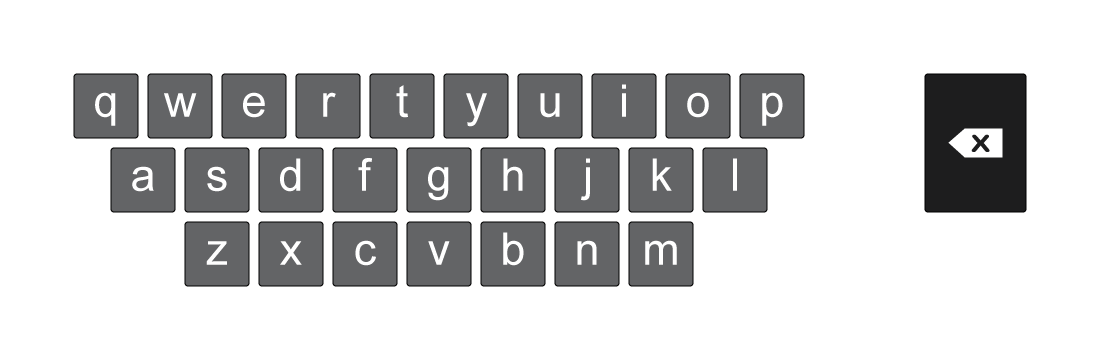
\includegraphics[width=6in]{fig_final_keyboard}
	\caption[Display: Keyboard Layout]{The keyboard layout used during the final study.}
	\label{keyboard_layout}
\end{figure}

\subsubsection{Text Area}
Figure~\ref{text_area} shows how two text areas were used to display text to participants. The top text-area showed the current word to transcribe, shown in Figure~\ref{text_a}, and the bottom area showed the currently transcribed text, shown in Figure~\ref{text_b}. The characters of both the displayed word and transcribed text were highlighted in green when the characters matched and were correct, whereas the letters in only the transcribed text would highlight in red if errors were made during transcription. The participant can then use the back space in order to correct words, and they are finally highlighted in green, as seen in Figure~\ref{text_c}, when a word was completed and correct.

\begin{figure}[b]
	\centering
	\begin{minipage}[t]{1.9in}
		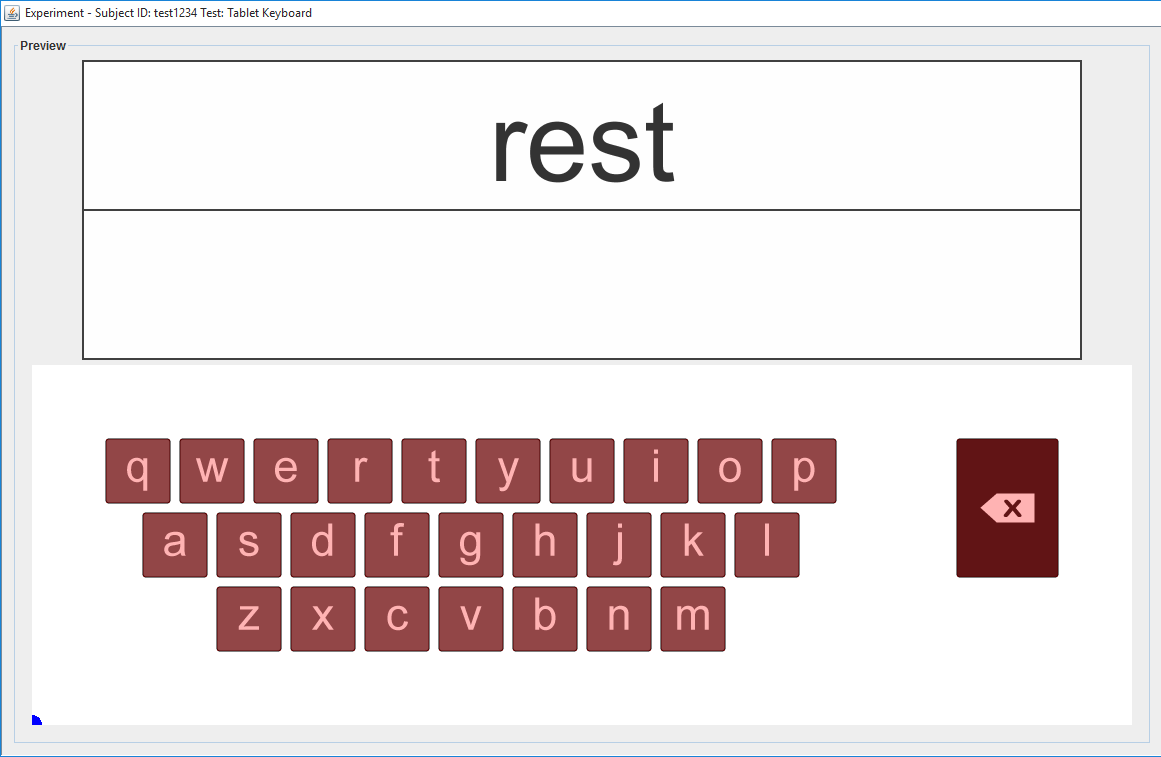
\includegraphics[width=2in]{fig_idle_keyboard}
		\subcaption{Displayed Word}
		\label{text_a}
	\end{minipage}
	\begin{minipage}[t]{1.9in}
		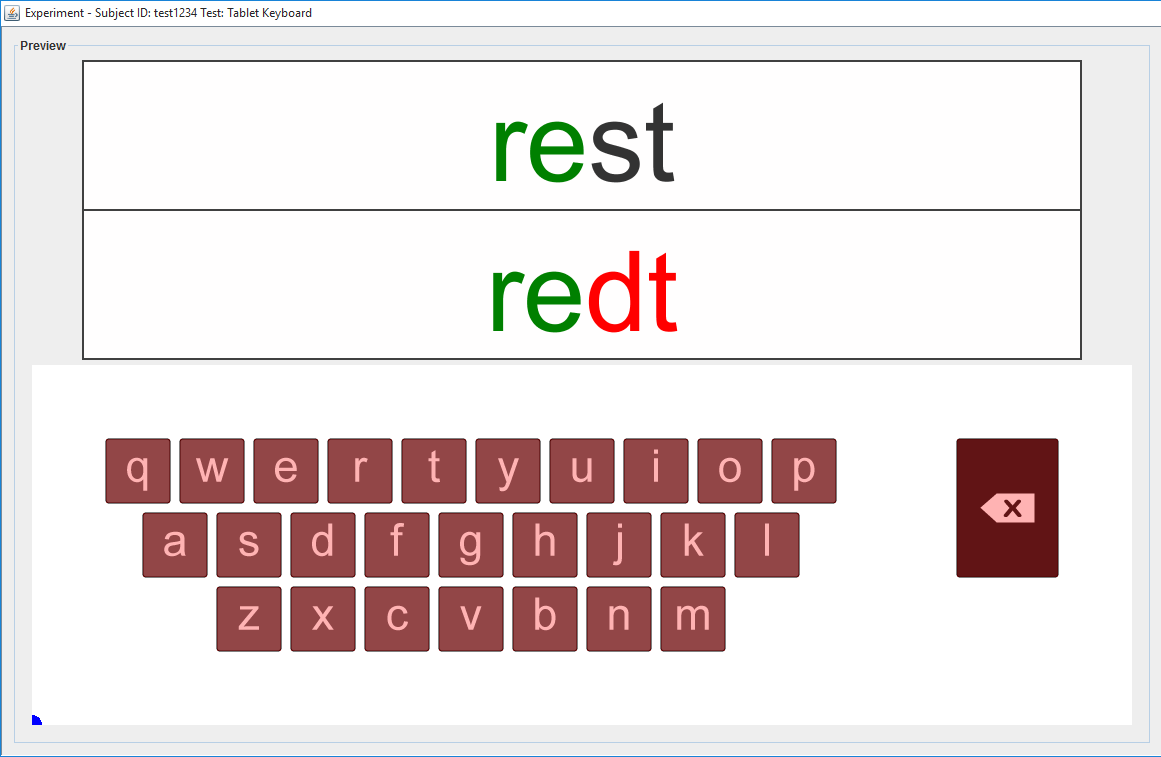
\includegraphics[width=2in]{fig_error_keyboard}
		\subcaption{Transcribed Error}
		\label{text_b}
	\end{minipage}
	\begin{minipage}[t]{1.9in}
		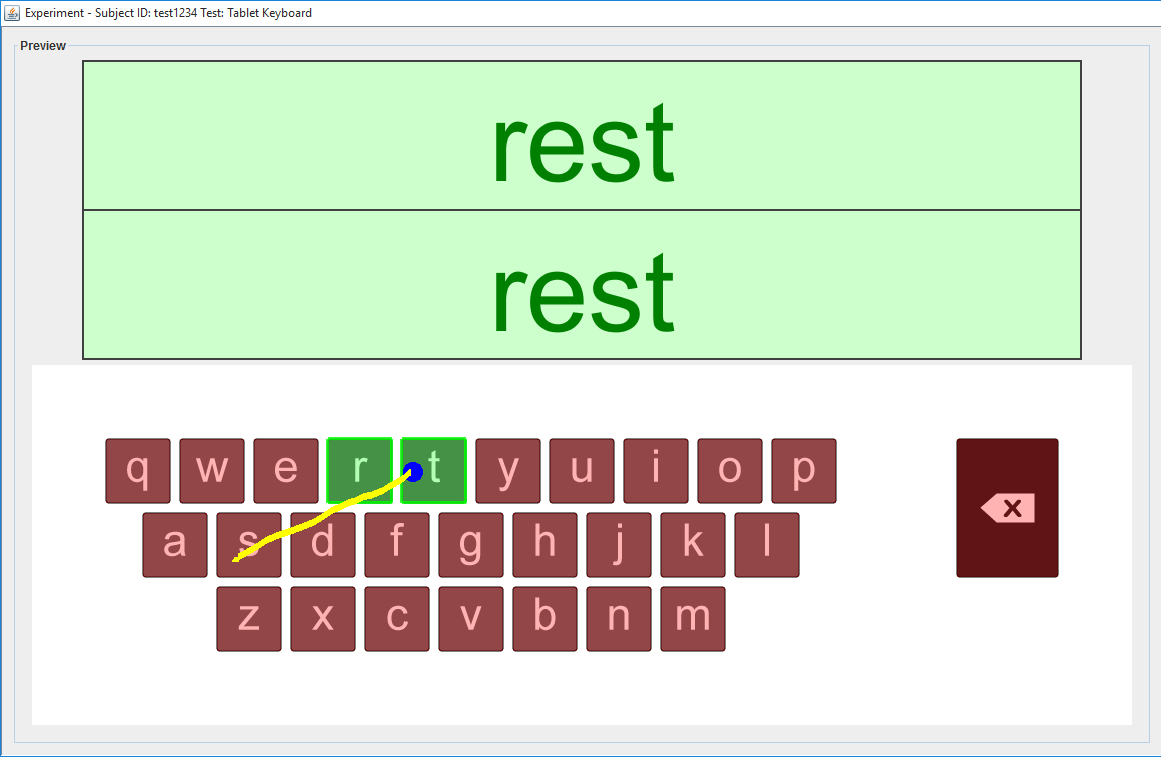
\includegraphics[width=2in]{fig_correct_keyboard}
		\subcaption{Completed Word}
		\label{text_c}
	\end{minipage}
	\caption[Display: Text Area]{Examples of how the text areas change when showing transcribed text. \textbf{(a)} shows the word to transcribe as it first appears. \textbf{(b)} shows how correct letters are highlighted green in both text areas and transcription errors are highlighted in red. \textbf{(c)} shows a completed word; the background lights up to indicate correctness.}
	\label{text_area}
\end{figure}

\subsubsection{Real-Time Updates}
As a participant is drawing the gesture-shape of a word, their progress is tracked in real time, as shown in Figure~\ref{display_area}. For the keyboards that track a participant's finger or the stylus, Figure~\ref{update_a} shows how a cylinder is displayed to indicate the direction that the finger is pointing, as well as which letter is being hovered over, indicated by a blue dot. As in Figure~\ref{update_b}, the participant is shown the path that they are traveling as well as the letters that have been pressed. The gesture-trail has a maximum length before it starts to decay as to not clutter the display. 

\begin{figure}[h]
	\centering
	\begin{minipage}[t]{2.9in}
		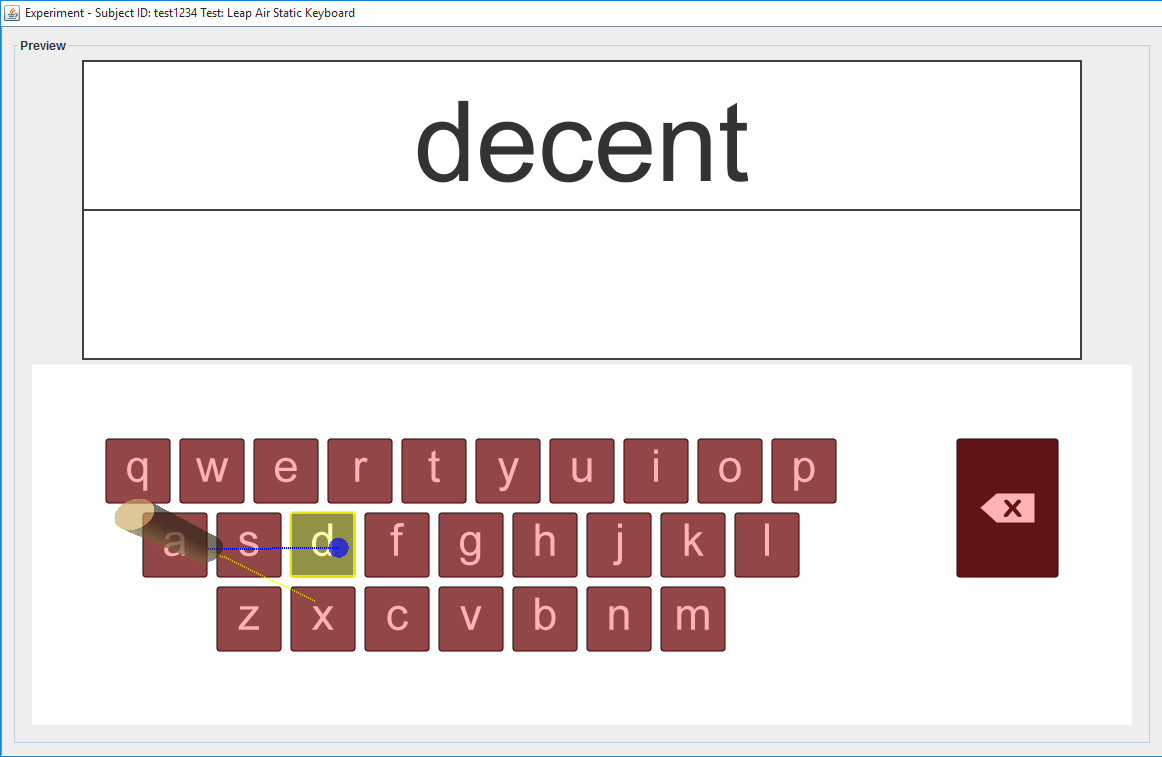
\includegraphics[width=3in]{fig_update1_keyboard}
		\subcaption{Prior to pressing 'd'}
		\label{update_a}
	\end{minipage}
	\begin{minipage}[t]{2.9in}
		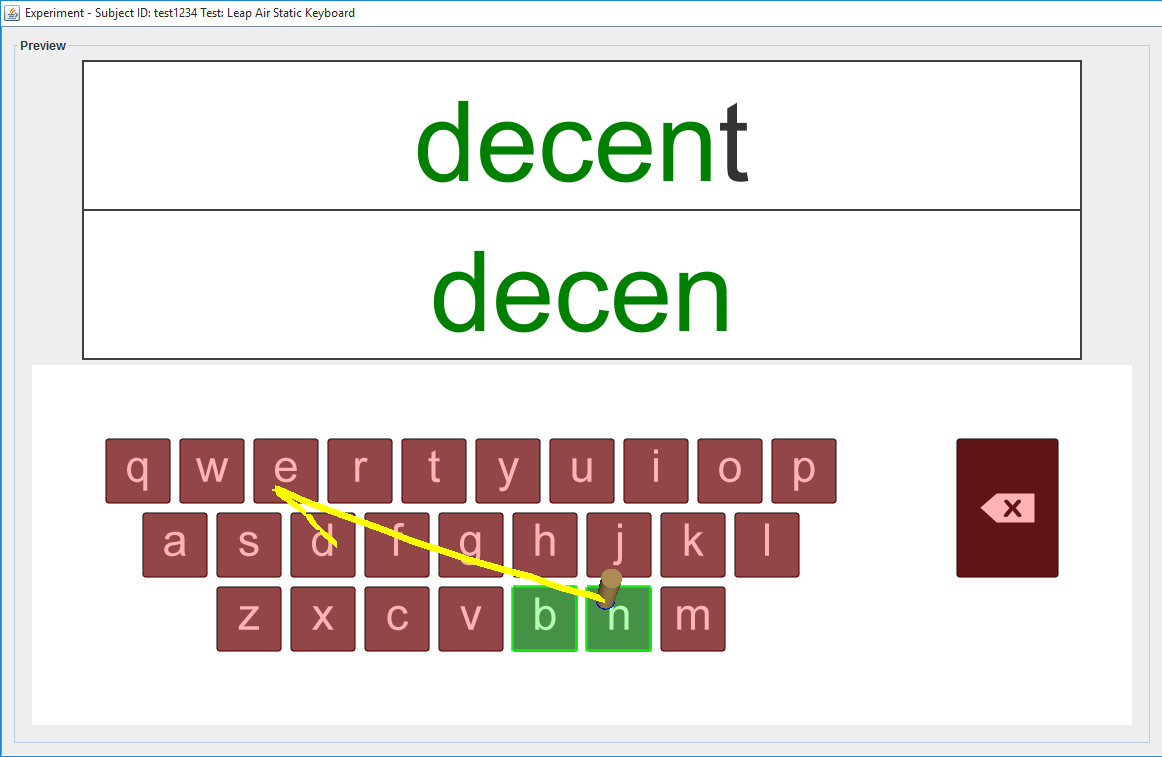
\includegraphics[width=3in]{fig_update2_keyboard}
		\subcaption{During the word-gesture}
		\label{update_b}
	\end{minipage}
	\caption[Display: Real-time Updates]{Examples the real-time display for word-gesturing. \textbf{(a)} shows the user just about to press the first character. \textbf{(b)} shows the middle of the word gesturing process for the word "decent".}
	\label{display_area}
\end{figure}

\subsection{Calibration}
Each mid-air keyboard, including the Leap Surface Keyboard, had the ability to be calibrated in a similar manner as Personal Space \cite{ref_alvin_thesis}, seen in Figure~\ref{calibration_in_progress}. Many of the calibration spaces; however, had to be interacted with directly instead of projecting the participant's hand onto the interaction plane. Calibration was optional and a default calibration was used that worked okay for most people. Calibration had less of a lasting effect because the Leap Motion Controller was allowed to be repositioned which was sometimes a greater factor than the calibration itself. Because this study is not an accessibility study, participants were allowed to calibrate the keyboard with their arms rested or raised, not addressing the "Gorilla Arm Syndrome" mentioned in Section~\ref{gorilla_arm_syndrome}.

\begin{figure}[h]
	\centering
	\begin{minipage}[t]{4in}
		\begin{minipage}[t]{1.9in}
			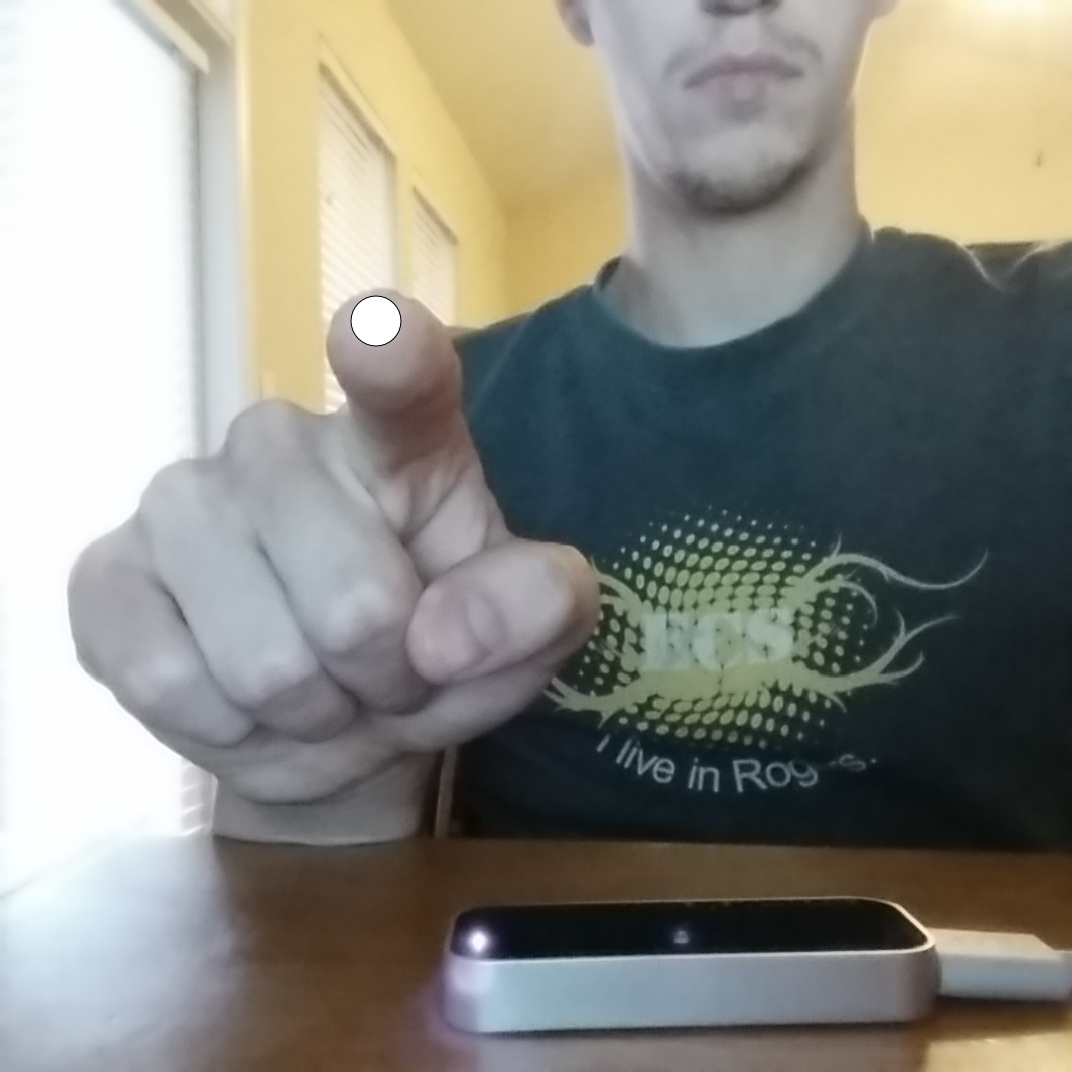
\includegraphics[width=2in]{fig_calib_1}
		\end{minipage}
		\begin{minipage}[t]{1.9in}
			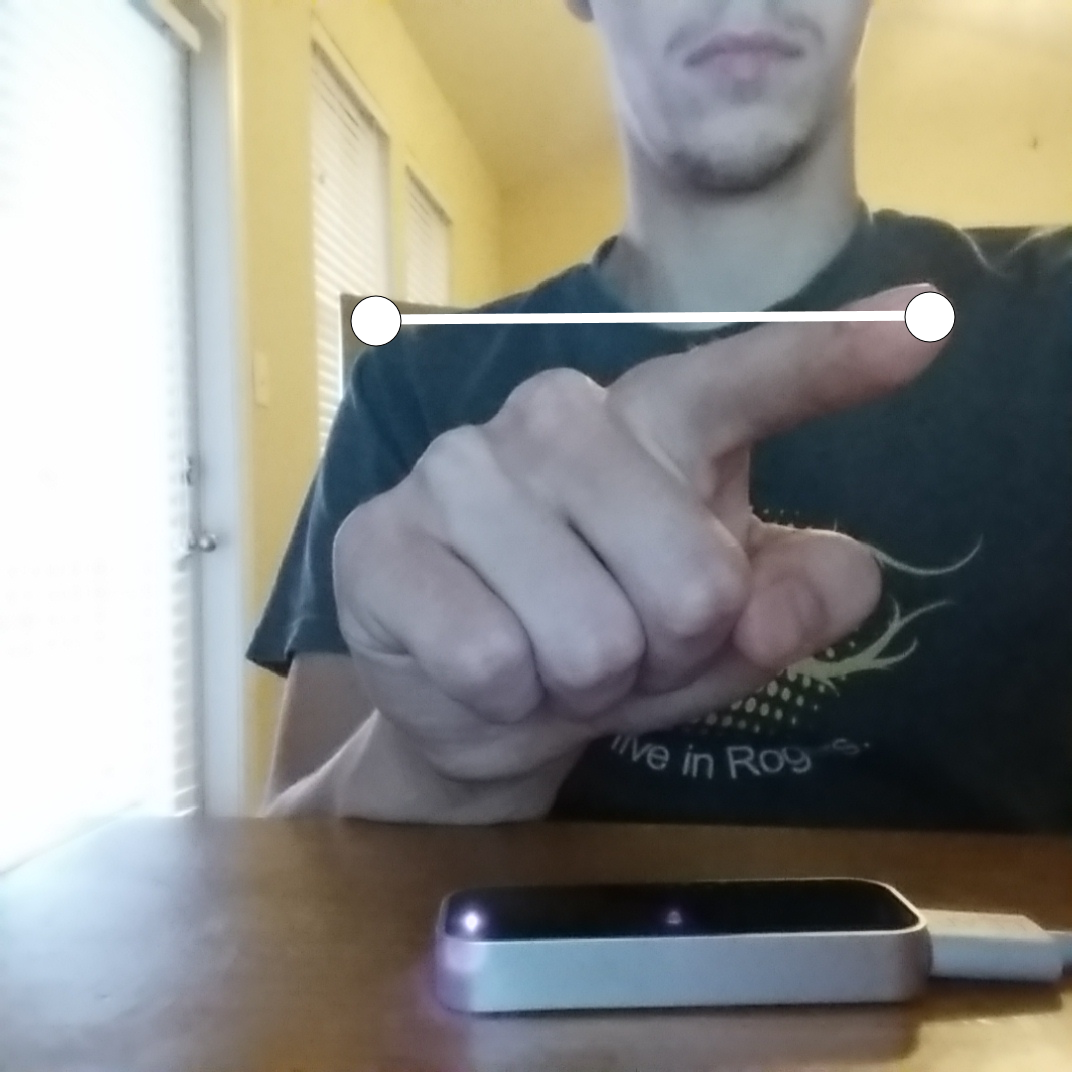
\includegraphics[width=2in]{fig_calib_2}
		\end{minipage}
	\end{minipage}
	
	\begin{minipage}[t]{4in}
		\begin{minipage}[t]{1.9in}
			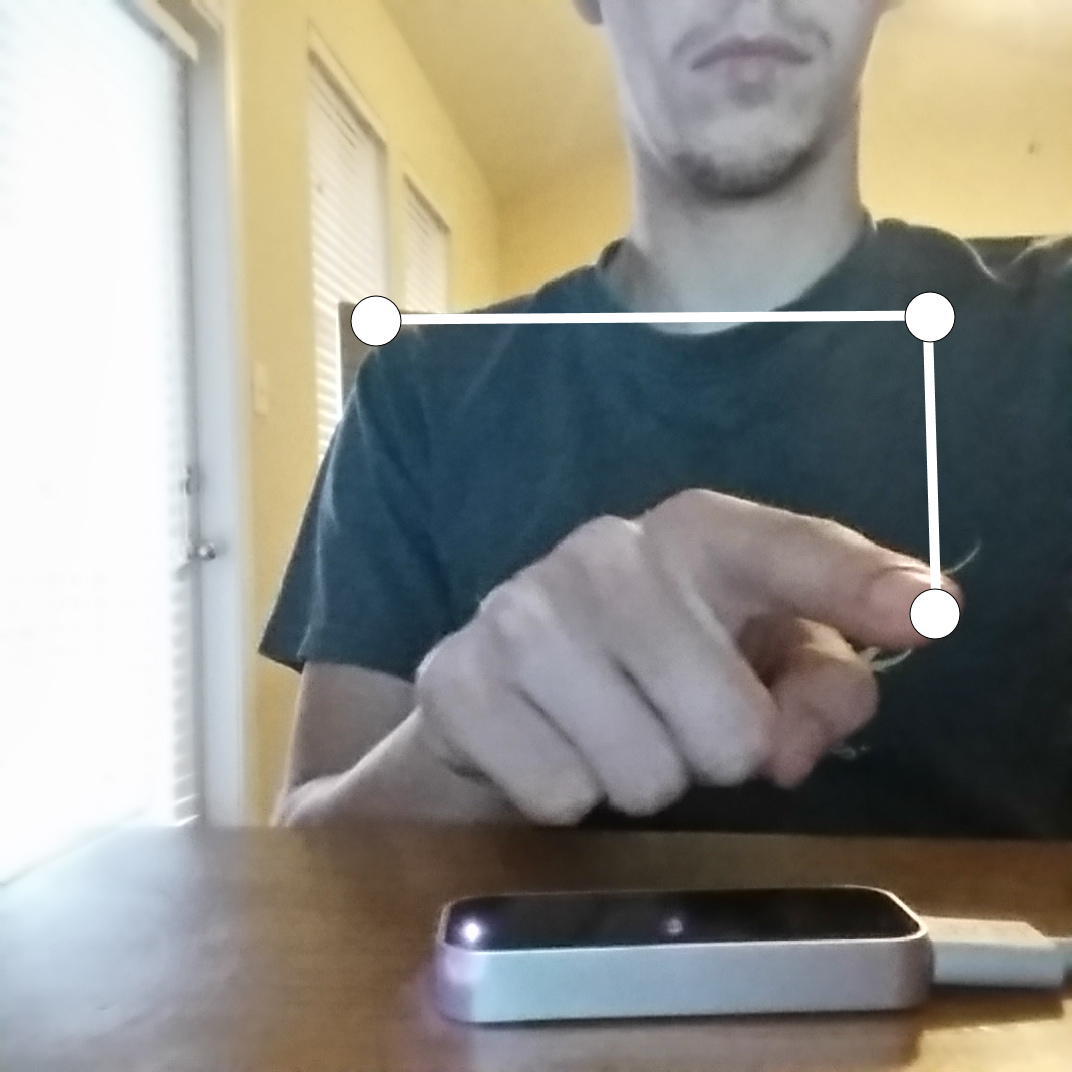
\includegraphics[width=2in]{fig_calib_3}
		\end{minipage}
		\begin{minipage}[t]{1.9in}
			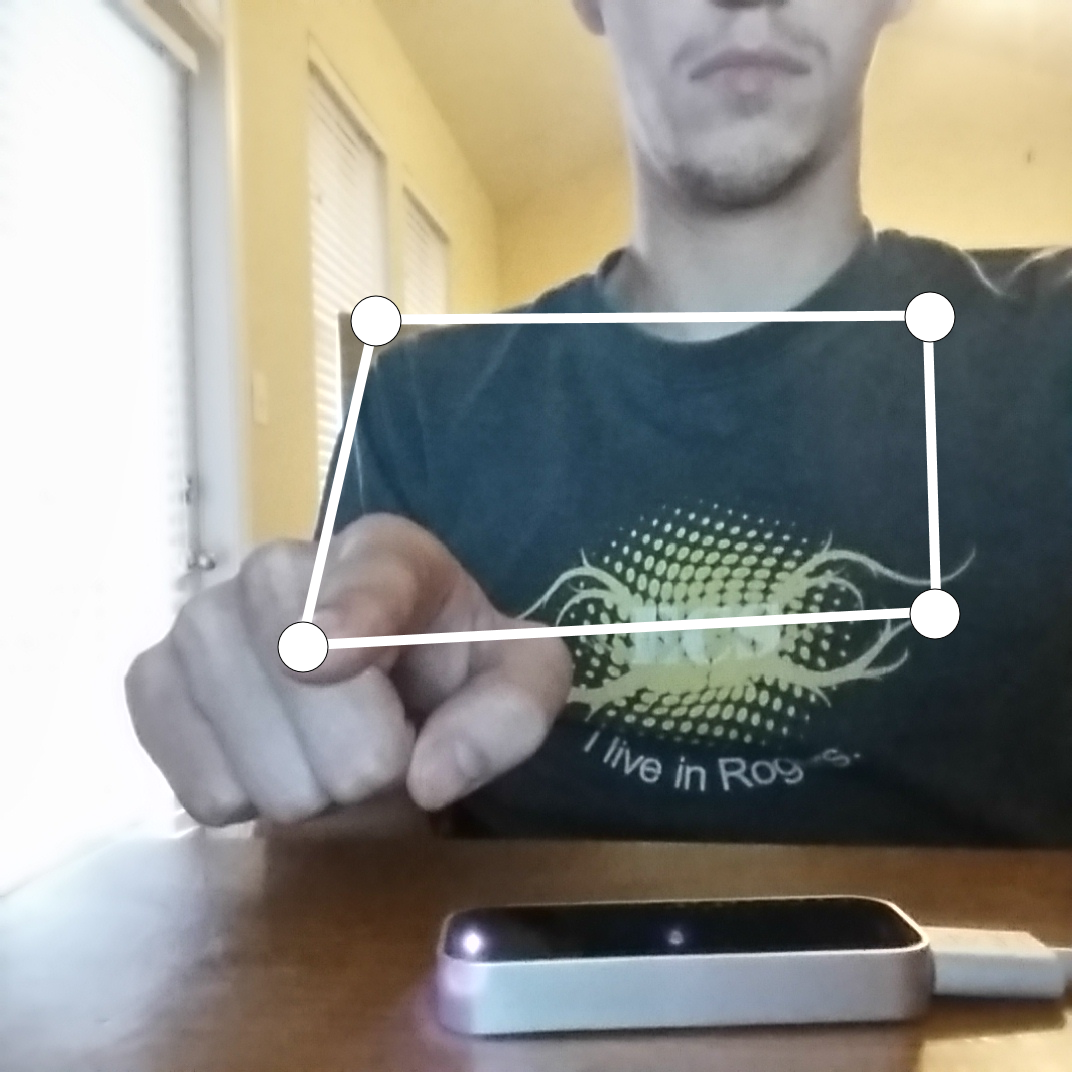
\includegraphics[width=2in]{fig_calib_4}
		\end{minipage}
	\end{minipage}
	\caption[Calibration]{Participants were able to follow on-screen instructions to calibrate the space interaction space using their finger.}
	\label{calibration_in_progress}
\end{figure}

\subsubsection{Motor Space and Display Space}
The calibrated interaction plane, or the motor space, was always attempted to be placed in near parallel to the screen, or display space; however, participants were allowed to move the Leap Motion Controller around to a position that felt best to them. Moving the Leap Motion Controller typically ended up with the motor space being oriented perpendicularly to the participants' arms rather than the display space. Also to note, when working with keyboards that fully utilized the 3rd-Dimension, an interaction plane angled away from the participant was sometimes more effective than a straight plane that was perpendicular to the ground. Figure~\ref{plane_angle} shows the difference between a straight plane and angled plane.

\begin{figure}[h]
	\centering
	\begin{minipage}[t]{4in}
		\begin{minipage}[t]{1.9in}
			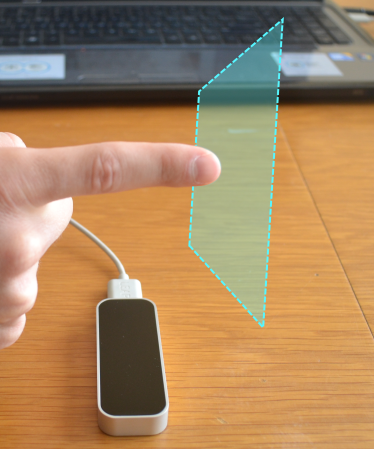
\includegraphics[width=2in]{fig_plane_straight}
			\subcaption{Straight Plane}
		\end{minipage}
		\begin{minipage}[t]{1.9in}
			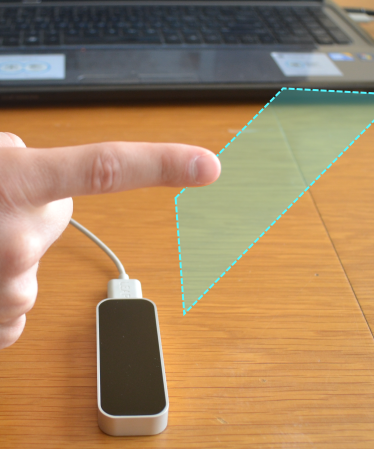
\includegraphics[width=2in]{fig_plane_angled}
			\subcaption{Angled Plane}
		\end{minipage}
	\end{minipage}
	\caption[Angled Plane]{Examples of a straight plane versus an angled plane.}
	\label{plane_angle}
\end{figure}

The size of the motor space was dependent on the device being used or the calibration of the keyboard's interaction plane. For all of the keyboards, the motor space was mapped to a display space with the size of 952x212 pixels and keys that were 64x64 pixels with gaps of 10 pixels. The real-world size of the display was dependent on the screen being used. Figure~\ref{motor_space_size} shows the average sizes of the motor spaces.

\begin{figure}[h]
	\centering
	\begin{minipage}[t]{2.5in}
		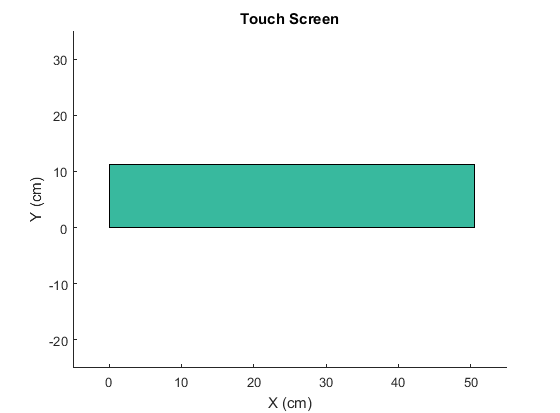
\includegraphics[width=2.5in]{fig_calibration_touch}
		\subcaption{Touch Screen}
		\label{fig_calibration_touch}
	\end{minipage}
	\begin{minipage}[t]{2.5in}
		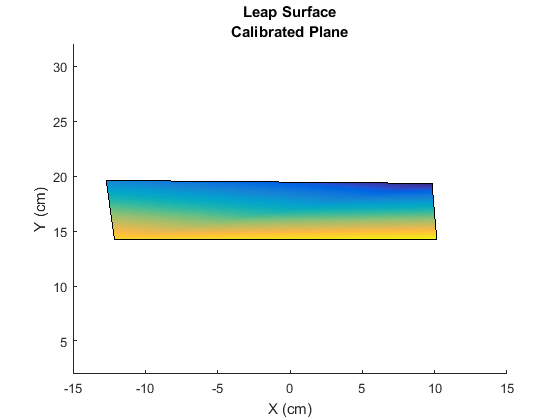
\includegraphics[width=2.5in]{fig_calibration_surface}
		\subcaption{Leap Surface}
		\label{fig_calibration_surface}
	\end{minipage}
	\begin{minipage}[t]{2.5in}
		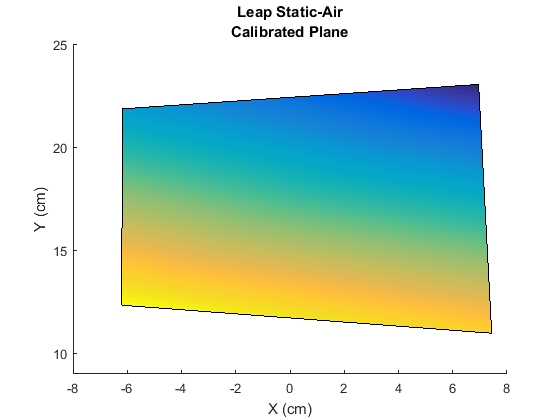
\includegraphics[width=2.5in]{fig_calibration_static}
		\subcaption{Static/Predictive/Bimodal}
		\label{fig_calibration_static}
	\end{minipage}
	\begin{minipage}[t]{2.5in}
		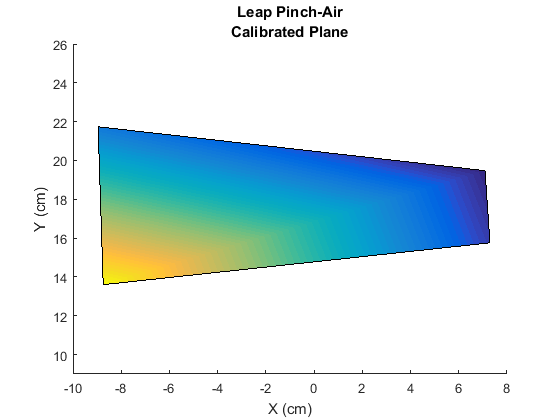
\includegraphics[width=2.5in]{fig_calibration_pinch}
		\subcaption{Leap Pinch-Air}
		\label{fig_calibration_pinch}
	\end{minipage}
	\caption[Motor Space Comparison]{The average size of the motor spaces for each keyboard with a gradient color scale showing the plane orientation. The closest \textbf{yellow} and furthest \textbf{blue}. \textbf{(a)} shows the standard Touch Sceen motor space. \textbf{(b)} shows the average calibration for the Leap Surface motor space. \textbf{(c)} shows the average calibration for the Leap Static-Air, Predictive-Air, and Bimodal-Air motor spaces (typically one was used for all three). \textbf{(d)} shows the average calibration for the Leap Pinch-Air motor space.}
	\label{motor_space_size}
\end{figure}

\subsection{Dictionary Creation} \label{dictionary_creation}
To make each keyboard experience as similar as possible, custom dictionaries were created for each keyboard input device containing words with similar gesture-shapes between keyboards. Dictionaries were created using a custom gesture-shape dissimilarity algorithm. The dictionaries contained words between the character lengths of 3 and 6 so that words would be rather simple, and words that most participants had seen before.

\subsubsection{Using Similar Gesture-Shapes}
The reason that custom dictionaries were chosen to be created was because it was thought that dependent measures would be more accurately represented for each keyboard if the experiences between those keyboards was nearly the same, only changing due to implementation. There was no previous research on words with similar gesture-shapes, or if this was truly necessary or beneficial.

\subsubsection {Gesture-Shape Dissimilarity}
Originally the Fr\'echet Distance was used to try to find the most similar word gesture-shapes using the sets of words with the least distance between each gesture-shape. Fr\'echet Distance gave acceptable results, however there were noticeable differences in some of the paths created.

In order to achieve gesture-shapes with even closer similarity, a custom dissimilarity algorithm to rate words' gesture-shapes of the same length was created. The top results for words with the least dissimilarity between each other were then split among the dictionaries. The dissimilarity between two words is defined by the formula
\begin{equation}
dissimilarity(P,\ Q) = \frac{\sum\limits_{i = 2}^{N} \frac{1}{2} \left(\left(\frac{\mid dist(P_{i},\ P_{i-1}) - dist(Q_{i},\ Q_{i-1})\mid}{max\ distance}\right) + \left(\frac{angle(P_{i} - P_{i-1},\ Q_{i} - Q_{i-1})}{\pi}\right)\right)}{N - 1}
\end{equation}
where $P$ and $Q$ were two words of $N$ length, $P_i$ and $Q_i$ were the vector locations of the characters of the words on the virtual keyboard, $max\ distance$ was the maximum distance between any two letters on the virtual keyboard, $dist(...)$ was the distance between two vector locations, and $angle(...)$ was the angle between two vectors. The dissimilarity formula forced values between the range [0, 1] and treated every pair of paths between two letters of two words with equal weight. The objective was then to find the sets of words with the lowest dissimilarity.

\section{Word-Gesture Keyboards}
All of the word-gesture keyboards created used the same word-gesturing implementation but differentiated by their interaction method and how touch simulation was handled as a delimiter between words.

\subsection{Touch Screen Keyboard}
\subsubsection{Interaction Method}
The Touch Screen Keyboard was implemented to mirror the de facto method for word-gesture keyboards which are touch-based. The user interacts directly with a touch screen surface.

\subsubsection{Word Separation}
Figure~\ref{touch_screen_press_comparison} shows that word separation for the Touch Screen Keyboard worked in the same way as typical word-gesture keyboards for phones and tablets. Touch was simulated simply by pressing a finger against the surface, drawing the word-gesture, and then removing the finger from the surface.

\begin{figure}[h]
	\centering
	\begin{minipage}[t]{5.8in}
		\begin{minipage}[t]{2.85in}
			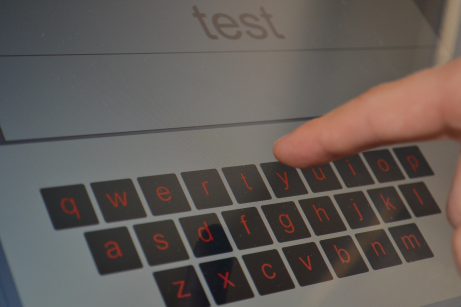
\includegraphics[width=2.9in]{fig_touch_screen_hover}
		\end{minipage}
		\begin{minipage}[t]{2.9in}
			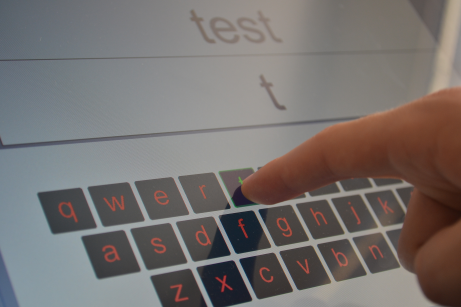
\includegraphics[width=2.9in]{fig_touch_screen_press}
		\end{minipage}
	\end{minipage}
	\caption[Touch Screen Word Separation]{A touch is simulated when the tabletop screen is touched.}
	\label{touch_screen_press_comparison}
\end{figure}

\subsubsection{Size of the Motor Space}
The motor space for the Touch Screen Keyboard was larger than the other keyboards because it utilized the Ideum Multi-touch Table Platform 46" tabletop, shown in Figure~\ref{fig_ideum}, which had a maximum resolution of 1920x1080 pixels. When scaled for the maximum resolution, the Touch Screen display space and motor space were both 50.49x11.24 $cm$, with keys that were 3.39x3.39 $cm$ and gaps between keys of 0.53 $cm$. If higher resolutions were available, a higher resolution would have been chosen to decrease the overall size of the display space and motor space to match the other keyboards more closely. Though larger than desired, the Ideum Multi-touch Table Platform was still preferred over using very small touch-keyboards such as those on phones or tablets. Having similar sized motor spaces was to help standardize results between touch and mid-air.

\begin{figure}[h]
	\centering
	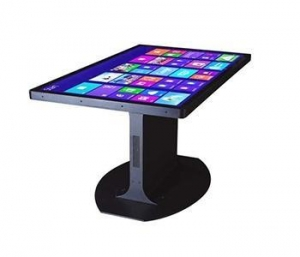
\includegraphics{fig_ideum}
	\caption[Ideum Multi-touch Table Platform]{The Ideum Multi-touch Table Platform tabletop.}
	\label{fig_ideum}
\end{figure}

\subsection{Leap Surface Keyboard} \label{leap_surface}
\subsubsection{Interaction Method}
The Leap Surface Keyboard used the Leap Motion Controller to track a wooden stylus for interaction. It was designed so that it would simulate a touch screen using a mid-air plane projected onto a surface. This was done by inserting the Leap Motion into a custom holder, shown in Figure~\ref{fig_leap_holder}, and projecting the mid-air keyboard over a keyboard printed on paper. As an added note, the Leap Surface Keyboard works in the exact same way as the Static-Air Keyboard in Section~\ref{static_air} except for that it is calibrated to a surface rather than mid-air. A stylus was chosen to be used as an interaction tool for this setup to allow for accurate surface emulation because the Leap Motion Controller was in a position that made it difficult to successfully track a participants hand or finger. Unfortunately, the Leap Controller had to be positioned in the way that it was because the hardware, at the time of implementation, was not designed to recognize hands from the other direction, or otherwise "upsidedown".

\begin{figure}[h]
	\centering
	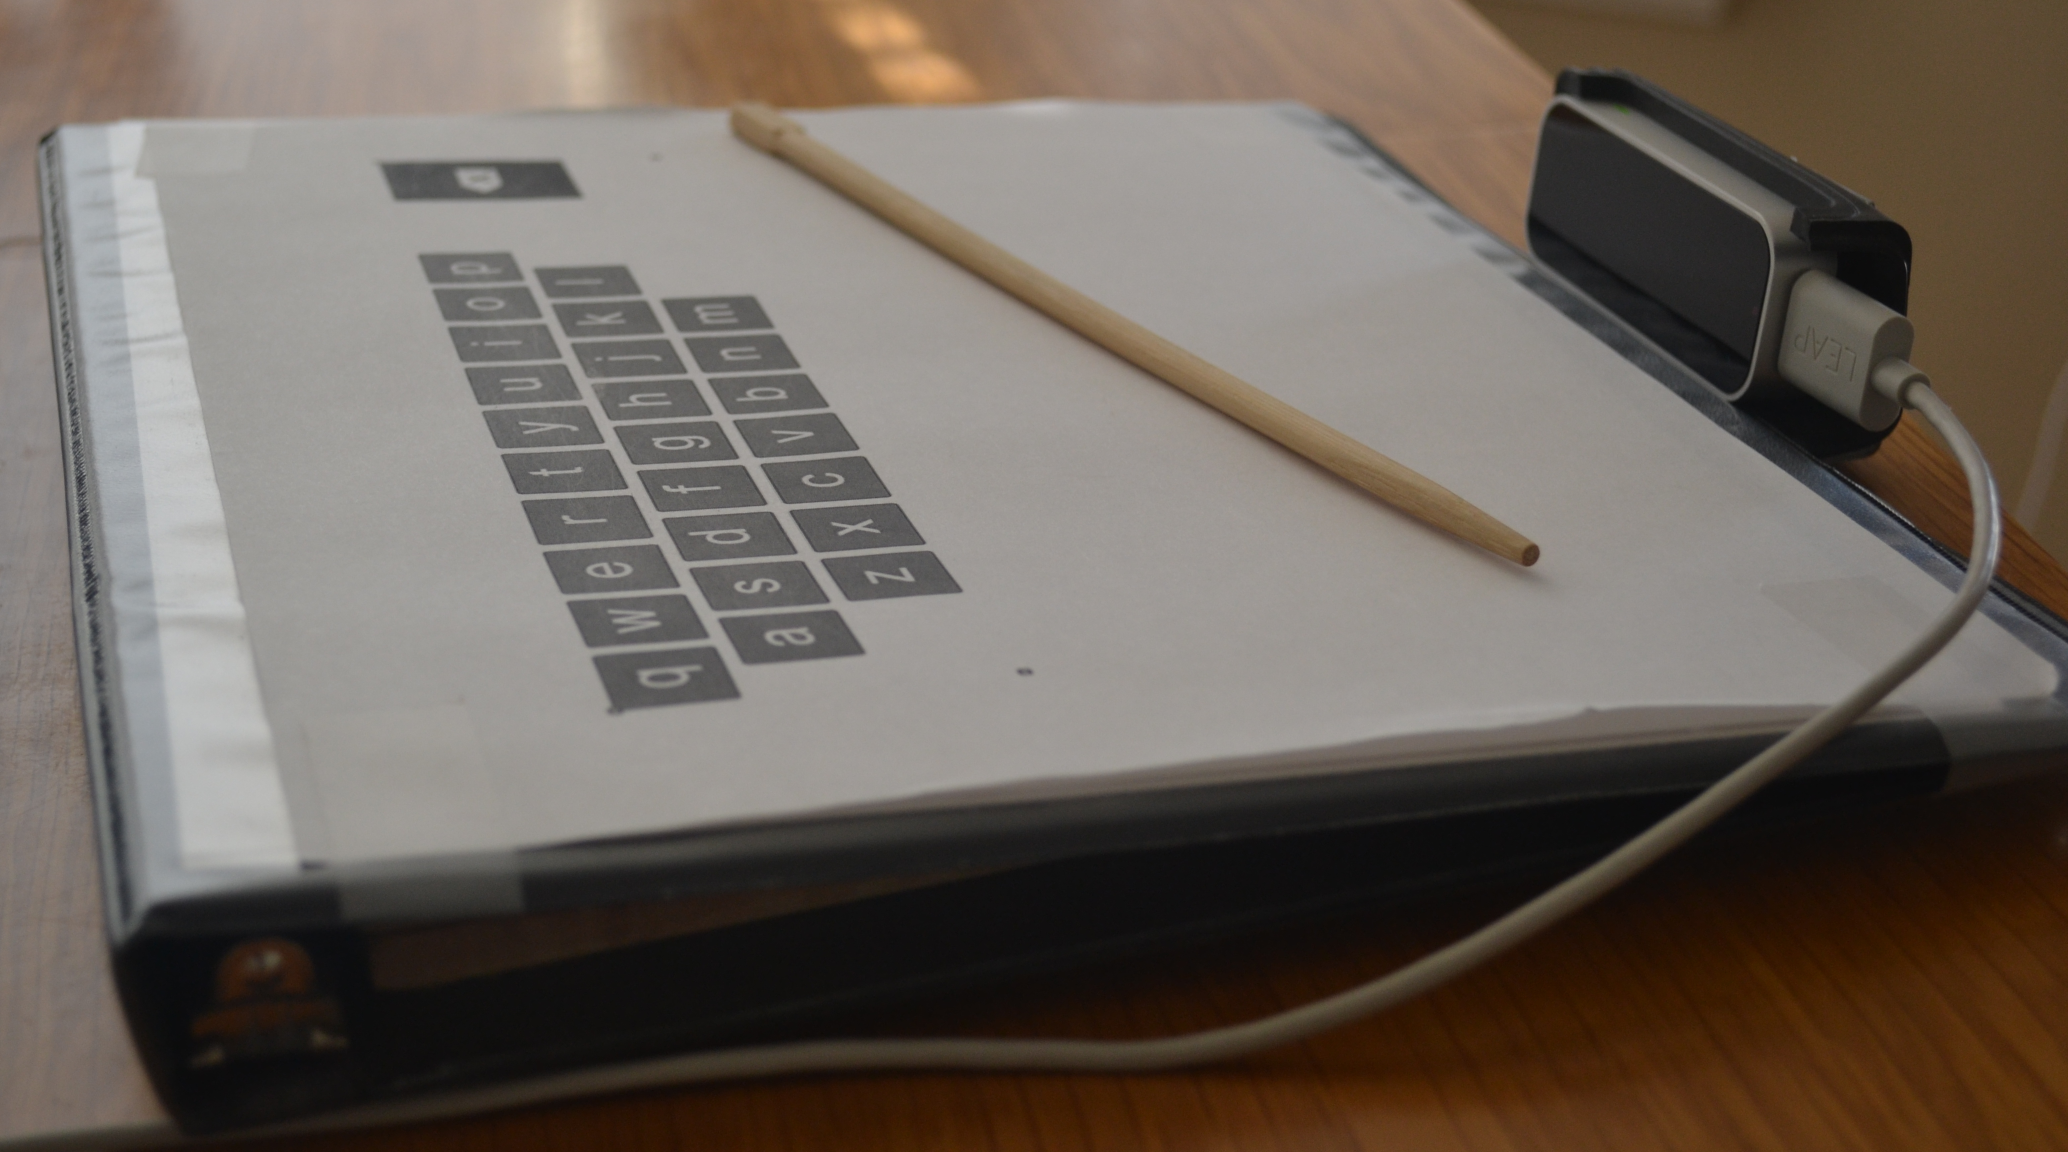
\includegraphics[width=5in]{fig_leap_holder}
	\caption[Leap Surface Holder]{The custom built holder, projecting an interaction plane onto a printed keyboard surface.}
	\label{fig_leap_holder}
\end{figure}

\subsubsection{Word Separation}
Word separation for the Leap Surface Keyboard worked in a similar way to how touch is simulated using a stylus for a phone or tablet. Figure~\ref{leap_surface_press_comparison} shows how touch was simulated by pressing the tip of the stylus against the surface of the printed keyboard. The word-gestures was drawn and then the stylus removed from the surface to complete the action.

\begin{figure}[h]
	\centering
	\begin{minipage}[t]{5.8in}
		\begin{minipage}[t]{2.85in}
			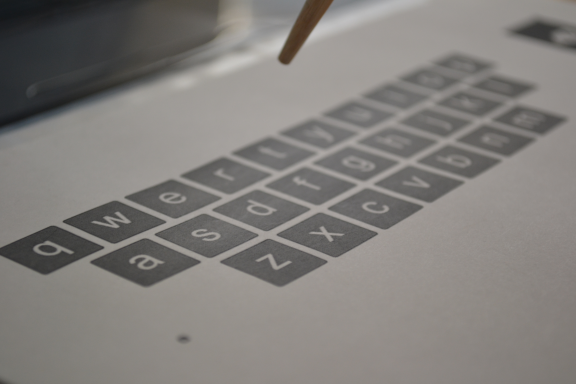
\includegraphics[width=2.9in]{fig_surface_hover}
		\end{minipage}
		\begin{minipage}[t]{2.9in}
			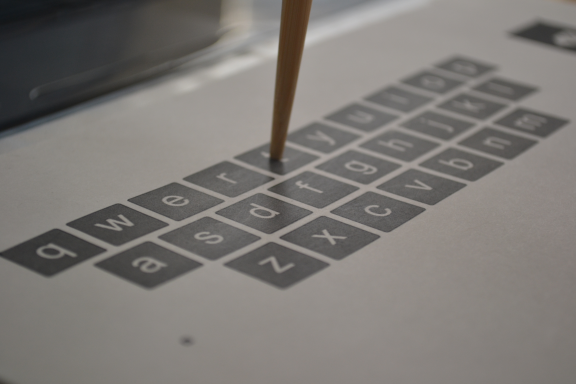
\includegraphics[width=2.9in]{fig_surface_touch}
		\end{minipage}
	\end{minipage}
	\caption[Leap Surface Word Separation]{A touch is simulated when the stylus hits the paper surface.}
	\label{leap_surface_press_comparison}
\end{figure}

\subsubsection{Size of the Motor Space}
Figure~\ref{fig_calibration_surface} shows the average calibrated motor space for the Leap Surface Keyboard. The average keyboard was 22.28x5.41 $cm$, with keys that were 1.50x1.50 $cm$ and gaps between keys of 0.23 $cm$.

\subsection{Leap Static-Air Keyboard} \label{static_air}
\subsubsection{Interaction Method}
The Leap Static-Air Keyboard used the Leap Motion Controller to track the pointer finger of either hand for interaction. It was designed so that it would simulate a touch screen in mid-air by projecting a quadrilateral plane in the air. The pointer finger would then be used to penetrate the plane to simulate touch.

\subsubsection{Word Separation}
Word separation for the Leap Static-Air Keyboard worked in a similar way as any ordinary touch-based word-gesture keyboard, however the simulated touch plane was in mid-air. Touch was simulated by using either pointer finger and penetrating the mid-air interaction plane as seen in Figure~\ref{static_press_comparison}. Then while maintaining the intersection, the pointer finger was used to draw the word-gesture, and then finally by pulling the finger away from the mid-air interaction plane, touch was released.

\begin{figure}[h]
	\centering
	\begin{minipage}[t]{5.8in}
		\begin{minipage}[t]{2.85in}
			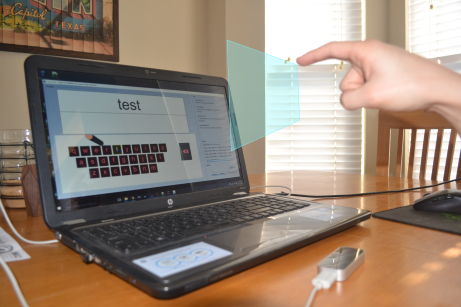
\includegraphics[width=2.9in]{fig_static_hover}
		\end{minipage}
		\begin{minipage}[t]{2.9in}
			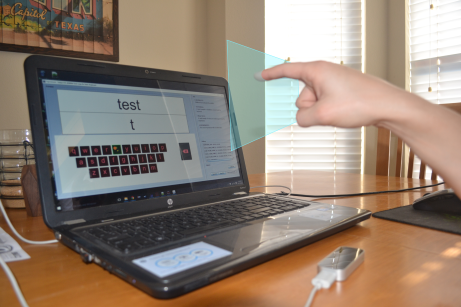
\includegraphics[width=2.9in]{fig_static_touch}
		\end{minipage}
	\end{minipage}
	\caption[Leap Static-Air Word Separation]{A touch is simulated by penetrating the interaction plane.}
	\label{static_press_comparison}
\end{figure}

\subsubsection{Size of the Motor Space}
Figure~\ref{fig_calibration_static} shows the average calibrated motor space for the Leap Static-Air Keyboard. The average keyboard was 13.71x10.07 $cm$, with keys that were 0.92x0.92 $cm$ and gaps between keys of 0.14 $cm$, the same as the Predictive-Air and Bimodal-Air keyboards.

\subsection{Leap Predictive-Air Keyboard}
\subsubsection{Interaction Method}
The Leap Predictive-Air Keyboard used the Leap Motion Controller to track the pointer finger of either hand for interaction. It was designed so that it would simulate a touch screen in mid-air by projecting a quadrilateral plane in the air; however, instead of having to interact with a static, unchanging plane, the Predictive-Air Keyboard associates the interaction plane with the participant's pointer finger. As the pointer finger moves forward or backward, the plane follows. The Predictive-Air Keyboard then tries to move the interaction plane to the pointer finger by predicting when a touch is being simulated by analyzing forward and backward hand gestures. Slow gestures serve mostly to move the plane, whereas quick gestures generally snap the pointer finger to the plane. The implementation of the forward and backward hand gestures are received from the base Leap Motion API.

\subsubsection{Word Separation}
Word separation for the Predictive-Air Keyboard worked in a similar way as any ordinary touch-based word-gesture keyboard, however the simulated touch plane is in mid-air. The mid-air interaction plane was kept at a static distance away from the detected pointer finger until a forward hand gesture was detected to simulate a touch. Once a touch was simulated, the pointer finger can then be used to draw the word-gesture until it is completed. Finally by making a backward hand gesture away from the interaction plane, the simulated touch is released. The plane interaction is visually similar to Figure~\ref{static_press_comparison}, the Leap Static-Air Keyboard interaction.

\subsubsection{Size of the Motor Space}
Figure~\ref{fig_calibration_static} shows the average calibrated motor space for the Leap Predictive-Air Keyboard. The average keyboard was 13.71x10.07 $cm$, with keys that were 0.92x0.92 $cm$ and gaps between keys of 0.14 $cm$, the same as the Static-Air and Bimodal-Air keyboards.

\subsection{Leap Bimodal-Air Keyboard}
\subsubsection{Interaction Method}
The Leap Bimodal-Air Keyboard used the Leap Motion Controller to track the pointer finger of either hand for interaction. It was designed by projecting a quadrilateral plane in the air and snapping the movements of the pointer finger to that plane. A touch was simulated by using a secondary input, in this case, a standard keyboard's space bar key.

\subsubsection{Word Separation}
Word separation for the Leap Bimodal-Air Keyboard worked by using a secondary input, the space bar. The interaction plane for simulated touch, as seen in Figure~\ref{bimodal_press}, was still projected in mid-air. Touch was simulated by using either pointer finger to determine the position over the interaction plane in the $x$-direction and $y$-direction and then by pressing and holding the space bar key to simulate touch. Then, while holding down the space bar, the pointer finger was used to draw the word-gesture and finally the space bar was released to end the touch.

\begin{figure}[h]
	\centering
	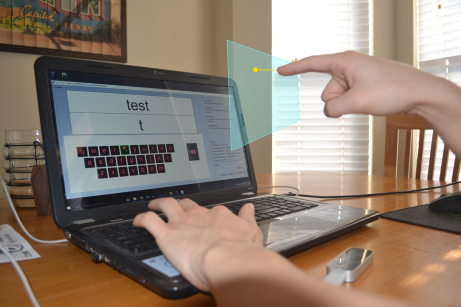
\includegraphics[width=5in]{fig_leap_bimodal}
	\caption[Leap Bimodal-Air Word-Separation]{A touch is simulated simply by pressing the space bar on the keyboard.}
	\label{bimodal_press}
\end{figure}

\subsubsection{Size of the Motor Space}
Figure~\ref{fig_calibration_static} shows the average calibrated motor space for the Leap Bimodal-Air Keyboard. The average keyboard was 13.71x10.07 $cm$, with keys that were 0.92x0.92 $cm$ and gaps between keys of 0.14 $cm$, the same as the Static-Air and Bimodal-Air keyboards.

\subsection{Leap Pinch-Air Keyboard}
\subsubsection{Interaction Method}
The Leap Pinch-Air Keyboard used the Leap Motion Controller to track the palm of either hand for interaction. It was designed in mid-air by projecting a quadrilateral plane in the air and snapping the palm position to the plane in the $z$-direction. The hand then could be used to form a pinch-gesture to simulate touch. The implementation of the pinch-gestures are received from the base Leap Motion API. It is important to note that unlike in Vulture \cite{ref_vulture}, no glove is required and many different pinch-gestures are recognized.

\subsubsection{Word Separation}
Word separation for the Leap Pinch-Air Keyboard worked by using a pinching-gesture; however, the interaction plane was still projected in mid-air. Touch was simulated by using either hand and then forming and holding a pinching-gesture, as shown in Figure~\ref{pinch_press_comparison}. While pinching, the word-gesture was drawn and then the pinching-gesture was released to end the touch.

\begin{figure}[h]
	\centering
	\begin{minipage}[t]{5.8in}
		\begin{minipage}[t]{2.85in}
			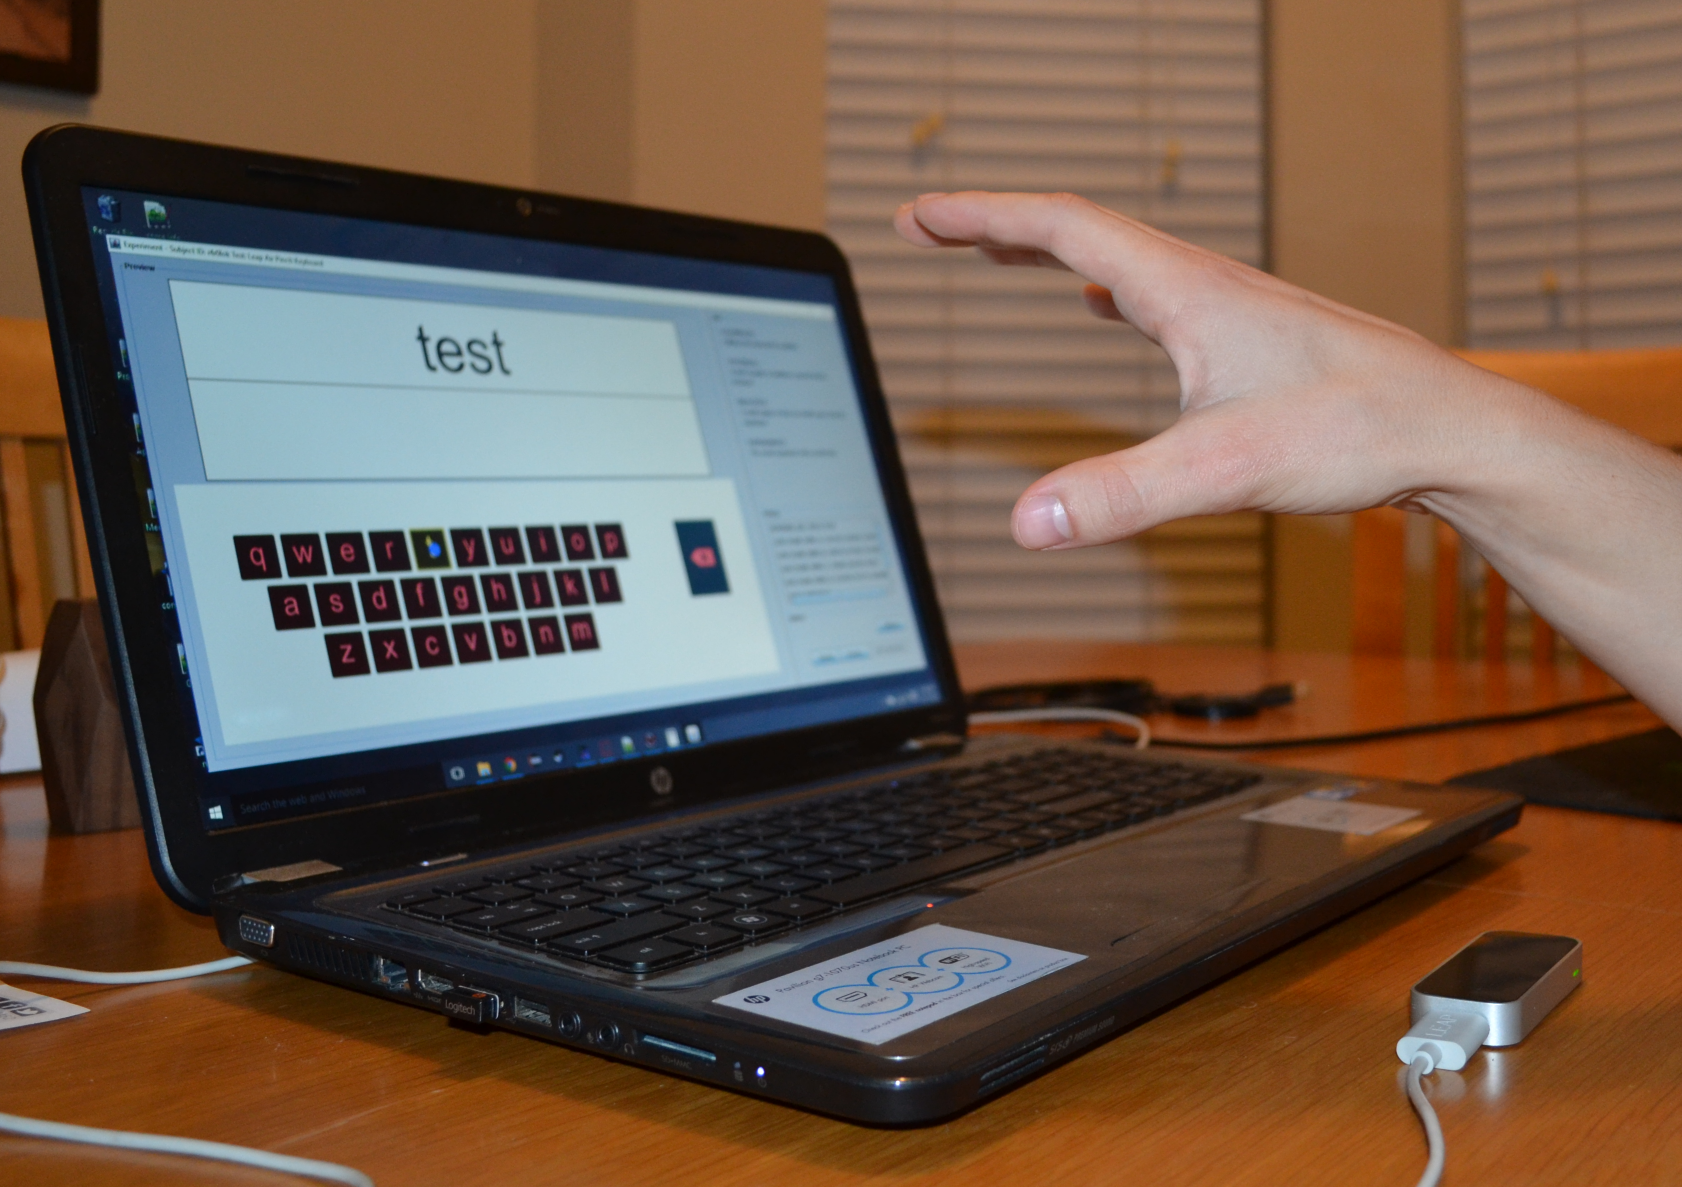
\includegraphics[width=2.9in]{fig_pinch_hover}
		\end{minipage}
		\begin{minipage}[t]{2.9in}
			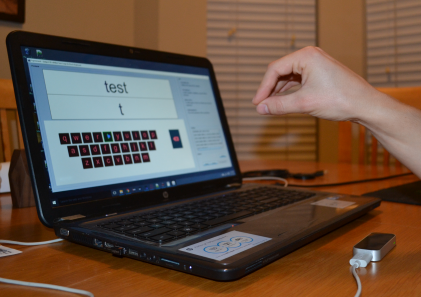
\includegraphics[width=2.9in]{fig_pinch_touch}
		\end{minipage}
	\end{minipage}
	\caption[Leap Pinch-Air Word Separation]{A touch is simulated by making a pinching gesture.}
	\label{pinch_press_comparison}
\end{figure}

\subsubsection{Size of the Motor Space}
Figure~\ref{fig_calibration_pinch} shows the average calibrated motor space for the Leap Pinch-Air Keyboard. The average keyboard was 16.86x9.04 $cm$, with keys that were 1.13x1.13 $cm$ and gaps between keys of 0.18 $cm$.
	\chapter{Pilot Studies} \label{pilot_studies}

\section{Pre-pilot Study} \label{pre_pilot}
The pre-pilot was a very informal study aimed at assessing the functionality of the pseudo word-gesture keyboard implementation. This informal study was used to also test the conceptual feasibility of using 3-dimensions as a means of word separation for simulated touch input. See Chapter~\ref{keyboard_design} for more specific implementation details.

\subsection{Participants} \label{pre_participants}
A sample size of 2 was used in the pre-pilot study. Both participants were male, ages 24 and 25 and both participants had previous experience with gesture-controllers, touch screens, and word-gesture keyboards. Table~\ref{pre_participant_stats} provides the participants' information in detail.

\begin{table}[!b]
	\centering
	\caption[Pre-pilot Study Details of Participants]{\centering Participant information including age, gender, handedness, computer usage, and previous experiences.}
	\label{pre_participant_stats}
	\resizebox{\textwidth}{!}{\begin{tabular}{ c | c c c c c c c c c c}
		\hline
		\multirow{2}{*}{Subject} & \multirow{2}{*}{Gender} & \multirow{2}{*}{Age} & Computer Usage & \multirow{2}{*}{Handedness} & Hand Used & Touch-device & Gesture-controller & Word-gesturing & Impairment \\
		{} & {} & {} & per Week (hours) & {} & in Experiment & Experience & Experience & Experience & History \\
		\hline
		1 & m & 24 & 31 - 40 & right & right & yes & yes & yes & no \\
		2 & m & 25 & 50+ & right & right & yes & yes & yes & no \\
		\hline
	\end{tabular}}
\end{table}

\subsection{Input Devices and Interaction Styles}
The interaction methods used within the pre-pilot study were dependent on the currently active keyboard input forcing the user to only interact with one style of keyboard at a time. All of the keyboards were simulated on a 64-bit Windows 7 work station, with all receivers or controllers connected via USB 2.0. The participants were allowed to recalibrate the active keyboard's interaction plane at any time before starting the main task for a more comfortable experience. Calibration was only possible if applicable to the active keyboard input. Participants were also encouraged to reposition the gesture-controller to best fit their personal preference and were given the option to freely rest or raise their elbows during the experiment. More information about the implementation of specific keyboard interactions and calibrations can be found in Chapter~\ref{keyboard_design}. Every keyboard was designed for use by either right or left handed participants. Figure~\ref{fig_old_keyboard} shows the keyboard layout used for all keyboards other than the Xbox Controller keyboard, whereas Figure~\ref{fig_xbox_keyboard} shows the keyboard used for the Xbox Controller Keyboard.

\subsubsection{Leap Motion Static-air Keyboard}
The Leap Motion Static-air Keyboard used a Leap Motion controller which was placed on the desk in front of the participant. The participant then used a stylus which was tracked by the Leap Motion controller in order to interact with a projected interaction plane. A touch was simulated by the insertion of the stylus into the interaction plane and a release was simulated upon the removal of the stylus. The interaction plane could be calibrated at any time prior to the experiment.

\begin{figure}[h]
	\centering
	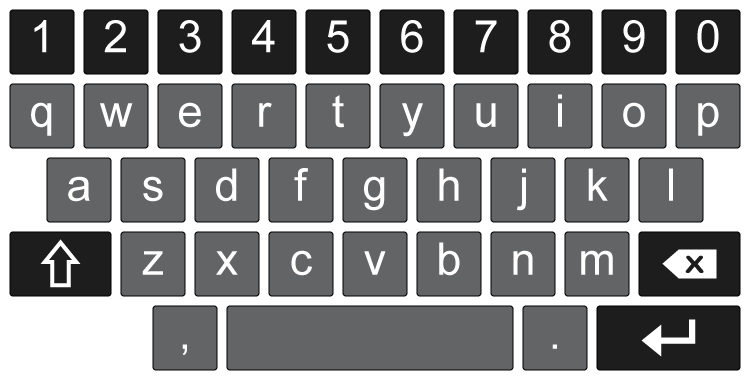
\includegraphics[width=6in]{Figures/fig_old_keyboard}
	\caption[Original Keyboard Layout]{The keyboard layout used during the pre-pilot study.}
	\label{fig_old_keyboard}
\end{figure}

\subsubsection{Leap Motion Pinch-air Keyboard}
The Leap Motion Pinch-air Keyboard also used a Leap Motion controller that was positioned on the desk in front of the participant. The participant then used their bare hand, which was tracked at the center of their palm, to interact with the projected interaction plane. Touch was simulated by having the participant make a pinching gesture with their hand and a release was simulated when the participant released the pinch, opening their hand again. As in the previous Static-air keyboard, the interaction plane could be calibrated at any time prior to the experiment.

\subsubsection{Leap Motion Surface Keyboard}
Again, for the Leap Motion Surface Keyboard, a Leap Motion controller was used for tracking. Unlike the Leap Static-air or Leap Pinch-air keyboards, the gesture controller was placed into a custom designed holder instead of on the desk in front of the participant. The holder was attached to an inclined surface with a printed keyboard fixed on top, as shown in Section~\ref{leap_surface}. Because identical placement was not guaranteed between uses, the Leap Motion Surface Keyboard required a single calibration after being inserted into the holder to accurately simulate an interaction plane projected onto the printed keyboard. The participant then used a stylus, as before, which was tracked by the Leap Motion controller in order to detect interaction. A touch was simulated by pressing the tip of the stylus against the printed keyboard and a release was simulated when the tip of the stylus was removed from the printed keyboard surface.

\subsubsection{Xbox Controller Keyboard}
The Xbox Controller Keyboard used an Xbox 360 Wireless Controller that transmitted information via the Microsoft Xbox 360 Wireless Receiver for Windows. The participants were required to use the directional sticks or the directional-pad in order to change which key was selected, and then used the `A' button in order to select the currently highlighted key. The Xbox Controller keyboard only allowed for single-input text entry, functioning in the same way as the default Xbox 360 virtual keyboard.

\begin{figure}[!t]
	\centering
	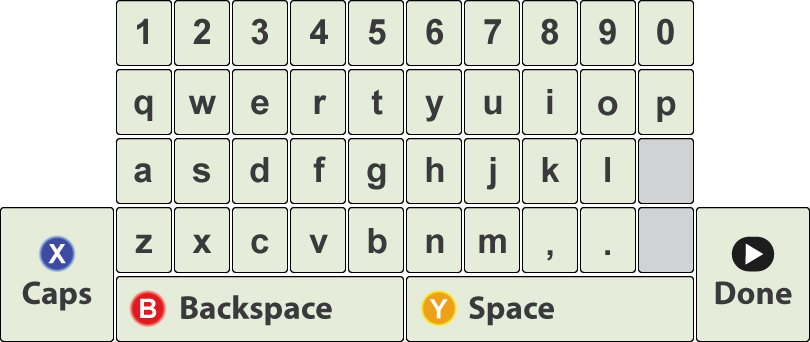
\includegraphics[width=6in]{Figures/fig_xbox_keyboard}
	\caption[Xbox Controller Keyboard Layout]{The keyboard layout used for the Xbox Controller Keyboard.}
	\label{fig_xbox_keyboard}
\end{figure}

\subsection{Task Design} \label{pre_task}
The design for the pre-pilot study included 4 different keyboard interaction styles representing each of the conditions that made up the task. The 4 conditions used were the Leap Motion Static-air, Leap Motion Pinch-air, Leap Motion Surface, and Xbox Controller keyboards.

The task consisted of 30 trials for each of the 4 keyboard interaction styles creating a total of 120 trials per participant. For each trial, a word of 3 to 6 characters in length was chosen at random from the Oxford English Dictionary and displayed on the screen. A blank text-area was positioned directly below the displayed word for the user-generated, transcribed text. Beneath both text areas, there was a virtual representation of the keyboard the participants were using. The participants were then required to use the currently active keyboard interaction style to enter the displayed word using word-gesturing. During the word-gesturing process, the participants were shown real-time updates to the displayed word and transcribed text as well as their movements within the virtual keyboard space. Detected key presses were appended directly to the transcribed text-area with correctly matching letters being colored green and text entry errors being colored red whereas only correctly matching letters were applied to the displayed word. The participants were required to use the active keyboard's backspace key to remove errors. Once a word was correctly entered, the participants were required to press the active keyboard's enter key to move on to the next word.

Small deviations in the above task were required for how the participants interacted with the Xbox Controller keyboard. For this keyboard, there was no word-gesturing feature implemented. Instead, the participant was asked to use single-input text entry using a standard Xbox 360 Controller. The Xbox Controller keyboard was implemented in the same way as a conventional console keyboard. The participants had to press the `A' button to select a letter, `Y' button to delete, and the `start' button to move to the next word.

\subsection{Experimental Design} \label{pre_experimental_design}
The initial pre-pilot study used a within-subjects design without any counterbalancing \cite{ref_within_subjects}. Both participants used every keyboard interaction style in a random order. The strength of a within-subjects design is the overall power increase and reduction in error variance associated with individual differences. The weakness of using the within-subjects design is that it suffers from ``carryover effects'' (the participation in one condition may affect performance in other conditions) between each keyboard interaction style.

\subsection{Procedure} \label{pre_procedure}
There was only a single study visit for each participant in which all tasks were performed. The study visit took between 30 and 45 minutes to complete depending on the number of calibrations. The full set of tasks and their expected durations are detailed in Table~\ref{pre_schedule_of_assessments}, the pre-pilot schedule of assessments. The participants followed the same process for each of the 4 keyboard interaction styles' tasks.

\begin{table}[!b]
	\centering
	\caption[Pre-pilot Study Schedule of Assessments]{\centering Schedule of Assessments for a single study visit during the pre-pilot study (in minutes).}
	\label{pre_schedule_of_assessments}
	\resizebox{\textwidth}{!}{\begin{tabular}{ l | c c c c c | c}
		\hline
		\multirow{2}{*}{Step} & \multirow{2}{*}{Controller} & Leap Motion & Leap Motion & Leap Motion & Exit & \multirow{2}{*}{Total}  \\
		{} & {} & Surface & Static-air & Pinch-air & Survey & {}  \\
		\hline
		explain & 0.5 & 0.5 & 0.5 & 0.5 & 0 & 2 \\
		practice & 5 & 5 & 5 & 5 & 0 & 20 \\
		calibrate & 0 & 2 & 2 & 2 & 0 & 6 \\
		task & 3 & 3 & 3 & 3 & 0 & 12 \\
		survey & 0 & 0 & 0 & 0 & 5 & 5 \\
		\hline
		Total & 8.5 & 10.5 & 10.5 & 10.5 & 5 & 45 \\
		\hline
	\end{tabular}}
\end{table}

First, the participants were given a brief verbal explanation and physical demonstration of the active keyboard input. The explanation dialog contained the name of the active keyboard and the method of interaction. The researcher then demonstrated how to enter the word ``test'' using the active keyboard. The participants were then given the stylus and control of interaction with the keyboard in order to become familiar with the interaction style.

Participants were then instructed to use the keyboard to perform practice words that were randomly chosen from the Oxford English Dictionary between 3 and 6 characters long. No practice words were duplicated and the dictionary was filtered for offensive words. There was no limit placed on how many words could be performed while practicing. The participants were told to continue until they felt they were able to efficiently and comfortably type each word with minimal errors. During the practice phase, the opportunity to optionally recalibrate the interaction-space any number of times was given if applicable to the active keyboard.

Next, the participants performed the task itself. As detailed in Section~\ref{pre_task}, the participants were instructed to enter a total of 30 words for the current keyboard interaction style. None of the experiment words were duplicated between themselves or the practice words and again were pulled at random from the Oxford English Dictionary between 3 and 6 characters, filtering for swear words. Participants were not allowed to recalibrate the interaction space during the task. 

After all tasks were completed for each of the 4 interaction styles, the participants were asked to fill out an exit survey. The exit survey asked the participants for their age, gender, major, and handedness as well as several questions detailing any prior touch, gesture-controller, or word-gesturing experience or impairments that might relate to the study. Finally, the participants were required to fill out the Likert scale relating to difficulty, discomfort, and fatigue experienced when using the interaction styles, as well as rank each interaction style on a numerical scale from best to worst.

\subsection{Dependent Measures}
The pre-pilot study collected qualitative testimonials alongside the exit survey. Participants were encouraged to give feedback of their experience during and after the experiment. The feedback was then used to refine the pseudo word-gesture keyboard implementation and assess the keyboard layout. Additionally, playback data from participants was also recorded. The playback data included detected key presses, the calibrated interaction plane, and the tracking location data. However, no empirical metrics intended for evaluating the keyboards' performances were observed.

\subsection{Pre-Pilot Summary}
The informal pre-pilot study allowed for assessing the functionality of the pseudo word-gesture keyboard implementation through qualitative feedback. The pseudo-implementation was observed to function adequately. In addition, many of the remaining bugs were revealed and corrected. The keyboard design was observed to be too cluttered; as a result, it was redesigned to be sleek and simple. Figure~\ref{fig_old_keyboard} shows the keyboard layout used in the pre-pilot study, whereas Figure~\ref{keyboard_layout} shows the final keyboard layout. A higher sensitivity to errors was observed after an initial error was made because path protection would be disabled; therefore, error correction was modified to be enforced for all later studies. A participant complained of fatigue during the study; for this reason, the number of trials was reduced for the pilot study.

\section{Pilot Study} \label{pilot}
The pilot study expanded on what was learned from the pre-pilot. Additional mid-air keyboard interactions were added and the displayed virtual keyboard was redesigned to be simpler and remove obtrusive features.

\subsection{Participants} \label{pilot_participants}
A sample size of 7 was used for the pilot study. There were 3 male and 4 female participants, ages ranging from 21 to 24 with a median age of 22. Participants' computer usage ranged from 6 to greater than 50 hours per week with a median usage of 21 to 30 hours per week. All of the participants described their right hand as being dominant and all participants used their right hand during the experiment except for one participant who switched back and forth. All of the participants had previous experience with touch devices. All but one participant had previous experience with gesture-controllers and only 57\% had previous experience with word-gesture keyboards. No participants had any impairment that affected their ability to enter text with computers. Table~\ref{pilot_participant_stats} provides the participants' information in detail.

\begin{table}[!b]
	\centering
	\caption[Pilot Study Details of Participants]{\centering Participant information including age, gender, handedness, computer usage, and previous experiences.}
	\label{pilot_participant_stats}
	\resizebox{\textwidth}{!}{\begin{tabular}{ c | c c c c c c c c c c}
		\hline
		\multirow{2}{*}{Subject} & \multirow{2}{*}{Gender} & \multirow{2}{*}{Age} & Computer Usage & \multirow{2}{*}{Handedness} & Hand Used & Touch-device & Gesture-controller & Word-gesturing & Impairment \\
		{} & {} & {} & per Week (hours) & {} & in Experiment & Experience & Experience & Experience & History \\
		\hline
		1 & male & 21 & 21 - 30 & right & right & yes & yes & no & no \\
		2 & male & 24 & 41 - 50 & right & right & yes & yes & yes & no \\
		3 & female & 22 & 50+ & right & right & yes & yes & yes & no \\
		4 & female & 23 & 50+ & right & right & yes & yes & yes & no \\
		5 & female & 21 & 6 - 10 & right & both & yes & yes & no & no \\
		6 & female & 24 & 6 - 10 & right & right & yes & no & no & no \\
		7 & male & 21 & 21 - 30 & right & right & yes & yes & yes & no \\
		\hline
	\end{tabular}}
\end{table}

\subsection{Input Devices and Interaction Styles}
The pilot study saw the introduction of three additional keyboard inputs: the Touch Screen Keyboard, the Leap Motion Bimodal-air Keyboard, and the Leap Motion Predictive-air Keyboard. The Touch Screen Keyboard was added because it is the de facto interaction for modern word-gesture keyboards \cite{ref_shape_writing}. The other two keyboards were added as alternative implementations to mid-air, word-gesture keyboards.

As in the pre-pilot, participants interacted with the different keyboard interaction styles one at a time. All of the keyboards except for the Touch Screen Keyboard were simulated on the same 64-bit Windows 7 work station as before. The Touch Screen Keyboard was simulated on the C4667PW, a 3M\textsuperscript{TM} Multi-touch Display, running 64-bit Windows 8. Again, all receivers or controllers were connected through USB 2.0. The participants were again allowed to recalibrate the active keyboard's interaction plane. Again, participants were encouraged to reposition the gesture-controller and were given the option to use either hand and rest or raise their arms during the experiment.

\subsubsection{Touch Screen Keyboard}
The Touch Screen Keyboard was used on a large tabletop touch screen. The participant then used their finger to interact with the virtual keyboard on the screen in the same way as typical touch devices. Touch was simulated when the participants finger touched the screen and release was simulated when the finger was lifted from the surface.

\subsubsection{Leap Motion Bimodal-air Keyboard}
The Leap Motion Bimodal-air Keyboard used a Leap Motion controller that was placed on the desk in front of the participant. The participant then used a stylus which was tracked by the Leap Motion controller in order to determine its location over the projected virtual keyboard. A touch was simulated by pressing the space bar key on a standard QWERTY keyboard and a touch release was simulated upon the release of the space bar. The interaction plane could be calibrated at any time prior to the experiment.

\subsubsection{Leap Motion Predictive-air Keyboard}
The Leap Motion Predictive-air Keyboard used a Leap Motion controller that was, again, placed on the desk in front of the participant. The participant then used a stylus, which was tracked by the Leap Motion controller, in order to interact with a projected interaction plane. A touch was simulated by recognizing and predicting a forward gesture of the stylus toward the interaction plane and a release was simulated by recognizing a backward gesture away from the interaction plane. As before, the interaction plane could be calibrated at any time prior to the experiment.

\subsection{Task Design} \label{pilot_task_design}
As in the pre-pilot, the conditions of the task were represented by the 7 different keyboard interaction styles. The 7 conditions used were the Leap Motion Static-air, Leap Motion Pinch-air, Leap Motion Surface, and Xbox Controller keyboards as before, with the addition of the Leap Motion Predictive-air, Leap Motion Bimodal-air, and Touch Screen keyboards.

Task profiles were created for each of the 7 keyboard interaction styles. Each task profile consisted of 10 separate trials for a total of 70 trials per participant. The reduction in trials from 30 words to 10 words for each keyboard was due to a complaint of fatigue during the pre-pilot study; one of the participants was unable to finish. The addition of task profiles were an attempt to standardize the data collected rather than randomizing words between uses of the same keyboard. Instead of choosing 10 words at random for each and every keyboard and participant, the task profiles insured that the same 10 words were used across each unique interaction style for all participants. This was handled by generating static, unchanging dictionaries for each keyboard, guaranteeing a total of 70 unique words as opposed to 490 unique words for the 7 participants. The 10 words selected for each dictionary were generated by a custom dissimilarity algorithm that produced the top 10 least dissimilar gesture-shapes across all words in the Oxford English Dictionary for words with 3 to 6 characters in length. This meant that only 10 different gesture-shapes were used by each participant across all interaction styles, ensuring that all participants' experiences with each keyboard were as similar as possible to each other and other participants. The creation of these dictionaries is detailed in Section~\ref{dictionary_creation}.

For each trial, a word was chosen at random from the active keyboard's previously constructed dictionary and displayed on the screen. A blank text-area was positioned directly below the displayed word for the participants' transcribed text. Beneath both text areas, the virtual representation of the previously displayed keyboard was updated and simplified. The shift, enter, and number keys were all removed, and the backspace key readjusted. The participants were then required to use the currently active keyboard interaction style to enter the displayed word using word-gesturing as before. During the word-gesturing process, participants were still shown real-time updates to the displayed word and transcribed text as well as their movements within the virtual keyboard space. The participants were required to use the active keyboard's backspace key to remove errors. However, already correctly transcribed characters were protected from being deleted. The change to protect the correctly transcribed characters was because of the high sensitivity and precision required to only delete the erroneous characters. Once a word was correctly entered, the participants were to release the simulated touch by the appropriate means of the active keyboard to move to the next word instead of hitting the enter key.

As before, deviations in the above task were required for how the participants interacted with the Xbox Controller keyboard. For this keyboard, there was still no word-gesturing feature implemented, instead the participant was asked to use single-input text entry using a standard Xbox 360 Controller. The participants had to press the `A' button to select a letter, `Y' button to delete, and the `start' button to move to the next word.

\subsection{Experimental Design} \label{pilot_experimental_design}
A within-subjects design was used for the pilot study \cite{ref_within_subjects}. The strength of a within-subjects design is the overall power increase and reduction in error variance associated with individual differences. The weakness of using the within-subjects design is that it suffers from ``carryover effects'' (the participation in one condition may affect performance in other conditions) between each keyboard interaction style. To account for this weakness, the study was supplemented with a Latin Squares design for counterbalancing \cite{ref_latin_squares}. Table~\ref{pilot_latin_squares} shows how the Latin Squares design was utilized for a sample size of 7 with an equal number of different keyboard inputs.
			
\begin{table}[!b] % b - for bottom; !t - for top
	\centering
	\caption[Latin Squares Example]{\centering Latin Squares design for 7 participants and 7 conditions.}
	\label{pilot_latin_squares}
	\begin{tabular}{c | c c c c c c c}
		\hline
		participants & \multicolumn{7}{c}{conditions} \\
		\hline
		1 & A & B & C & D & E & F & G \\
		2 & B & C & D & E & F & G & A \\
		3 & C & D & E & F & G & A & B \\
		4 & D & E & F & G & A & B & C \\
		5 & E & F & G & A & B & C & D \\
		6 & F & G & A & B & C & D & E \\
		7 & G & A & B & C & D & E & F \\
		\hline
	\end{tabular}
\end{table}

\subsection{Procedure} \label{pilot_procedure}
Each subject participated in a single study visit which took between 30 and 70 minutes to complete depending on how many calibrations were performed. The full set of tasks and their expected durations are detailed in Figure~\ref{pilot_schedule_of_assessments}, the pilot study schedule of assessments. The participants followed the same process for each of the 7 keyboard interaction styles' tasks.

\begin{table}[t] % b - for bottom; !t - for top
	\centering
	\caption[Pilot Study Schedule of Assessments]{\centering Schedule of Assessments for a single study visit during the pilot study (in minutes).}
	\label{pilot_schedule_of_assessments}
	\resizebox{\textwidth}{!}{\begin{tabular}{ l | c c c c c c c c | c}
		\hline
		\multirow{2}{*}{Step} & \multirow{2}{*}{Controller} & Touch & Leap Motion & Leap Motion & Leap Motion & Leap Motion & Leap Motion & Exit & \multirow{2}{*}{Total}  \\
		{} & {} & Screen & Surface & Static-air & Pinch-air & Predictive-air & Bimodal-air & Survey & {}  \\
		\hline
		explain & 0.5 & 0.5 & 0.5 & 0.5 & 0.5 & 0.5 & 0.5 & 0 & 3.5 \\
		calibrate & 0 & 0 & 2 & 2 & 2 & 2 & 2 & 0 & 10 \\
		practice & 5 & 5 & 5 & 5 & 5 & 5 & 5 & 0 & 35 \\
		task & 2 & 2 & 2 & 2 & 2 & 2 & 2 & 0 & 14 \\
		survey & 0 & 0 & 0 & 0 & 0 & 0 & 0 & 5 & 5 \\
		\hline
		Total & 7.5 & 7.5 & 9.5 & 9.5 & 9.5 & 9.5 & 9.5 & 5 & 67.5 \\
		\hline
	\end{tabular}}
\end{table}

First, the participants were given a brief verbal explanation and physical demonstration of the active keyboard input. The explanation dialog contained the name of the active keyboard and the method of interaction. The researcher then demonstrated how to enter the word ``test'' using the active keyboard. The participants were then given control of interaction with the keyboard in order to become familiar with the interaction style.

Participants were then instructed to use the keyboard to perform practice words which were randomly selected from the Oxford English Dictionary with lengths between 3 and 6 characters long. The practice words were filtered for offensive words and against the previously constructed experiment dictionaries so that no participants would be able to see any of the experiment words in advance. There was no limit placed on how many words could be performed while practicing. The participants were told to continue until they felt they were able to efficiently and comfortably gesture each word with minimal errors. During the practice phase, participants were given the opportunity to recalibrate the interaction-space if it was applicable for the currently active keyboard. Recalibration was allowed any number of times.

Next, the participants performed the task itself. As detailed in Section~\ref{pilot_task_design}, the participants were instructed to enter a total of 10 words for the current keyboard interaction style. The words selected were pulled at random from the active keyboard's previously constructed dictionary until all 10 words in the dictionary were used. Participants were not allowed to recalibrate the interaction space during the task. 

After all tasks were completed for each of the 7 interaction styles, the participants were asked to fill out an exit survey, shown in Appendix~\ref{surveys}. The exit survey asked the participants for their age, gender, major, and handedness as well as several questions detailing any prior touch, gesture-controller, or word-gesturing experience or impairments that might relate to the study. Finally, the participants were required to fill out the a Likert scale section relating to difficulty, discomfort and fatigue experienced when using the interaction styles as well as rank each style on a numerical scale from best to worst.

\subsection{Dependent Measures} \label{pilot_dependent_measures}
The design choice to not fully implement word-recognition for the word-gesture keyboards influenced the design of the task and therefore affected the dependent measures. Each individual trial was designed as a single word rather than a phrase that included many words, as in Vulture \cite{ref_vulture}. Therefore, most dependent measures were analyzed on the word-gesture level. It was possible to analyze these values at the phrase level if the combined trials were viewed as a single phrase.

\subsubsection{Text-entry rate}
Typically, text-entry rates were calculated using the standard Words Per Minute formula
\begin{equation}
WPM = \frac{|T-1|}{S} \times 60 \times \frac{1}{5}
\end{equation}
where $|T-1|$ was the length of the transcribed string and $S$ was the amount of time (in seconds) that was taken to transcribe the word from the time the first character was produced \cite{ref_wpm_word_gesture_formula}. When dealing with timing word-gestures, the formula must be modified to:
\begin{equation} \label{WPM}
WPM = \frac{|T|}{S} \times 60 \times \frac{1}{5}
\end{equation}
where $|T-1|$ was replaced with $|T|$ and $S$ represents the amount of time (in seconds) that was taken to transcribe the word including the time that it took to produce the first character. The modification was required because the time it takes to produce the first character must be included when timing word-gestures \cite{ref_wpm_word_gesture_timing}.

\subsubsection{Error rates}
There were several techniques used to measure error rates and find the best representation of keyboard performance and account for the task design.

The first error rate was modeled after the techniques in Vulture \cite{ref_vulture} and uses the Minimum Word Distance, which was calculated in the same way as the Minimum String Distance \cite{ref_error_rates,ref_vulture_MSD_ref}:
\begin{equation} \label{MWD}
MWD\ error\ rate = \frac{MWD(P,T)}{\overline{S_P}} \times 100\%
\end{equation}
Minimum Word Distance differentiated from Minimum String Distance in that it was calculated on a per-word level than on a per-character level where $P$ and $T$ were the sets of words in the presented and transcribed strings, and $\overline{S_P}$ was the mean size of the optimal alignments calculated on a per-word level \cite{ref_vulture}. It is important to note that because participants were forced to correctly type in words and there were no errors present in the final transcribed text, words that were considered erroneous had to be defined differently. For this thesis to take advantage of Minimum Word Distance, the word was counted as incorrect if the participant made any errors at all regardless of being forced to correct them. This gives the formula
\begin{equation} \label{MWD_simple}
MWD\ error\ rate = \frac{IW}{CW + IW} \times 100\%
\end{equation}
where $IW$ were words where the participant made any mistakes at all regardless of corrections and $CW$ were words where the participant got the word correct on the first attempt.

The next error rate used was the Keystrokes Per Character method, otherwise known as KSPC \cite{ref_error_rates}. The Keystrokes Per Character formula
\begin{equation} \label{KSPC}
KSPC \approx \frac{C + INF + IF + F}{C + INF}
\end{equation}
used Soukoreff and MacKenzie's keystroke taxonomy, where $C$ represented the correct characters in the transcribed text, $INF$ were the incorrect, not fixed characters in the transcribed text, $F$ was used to show the keystrokes which were editing functions (e.g., backspace), and $IF$ were the incorrect but fixed characters in the input stream. In consideration of $IF$, this did not include selecting backspace on accident. The Keystrokes Per Character method is less than ideal and has many limitations as an error metric \cite{ref_error_rates}. Yet, it was still beneficial to be used to analyze the rate of erroneous character production because the word-gesture keyboards were designed with a lack of true word-recognition. It is important to note that $INF$ always equated to zero, reducing Formula~\ref{KSPC} to
\begin{equation} \label{KSPC_simple}
KSPC \approx \frac{C + IF + F}{C}
\end{equation}
because the task required participants correctly transcribe each word before moving on to the next.

The final error rate used was the Total Error Rate \cite{ref_error_rates}. The Total Error Rate was also described by the previous keystroke taxonomy used in KSPC, giving the formula
\begin{equation} \label{TER}{
	Total\ Error\ Rate = \frac{INF + IF}{C + INF + F} \times 100\%
}
\end{equation}
where $C$ represented the correct characters in the transcribed text, $INF$ were the incorrect, not fixed characters in the transcribed text, $F$ was used to show the keystrokes which were editing functions (e.g., backspace), and $IF$ were the incorrect but fixed characters in the input stream. Once again, in consideration of $IF$, this did not include selecting backspace on accident. Again, Formula~\ref{TER} could be reduced to
\begin{equation} \label{TER_simple}
Total\ Error\ Rate = \frac{IF}{C + F} \times 100\%
\end{equation}
because participants were required to correctly transcribe words.

\subsubsection{Correctness} \label{pilot_correctness}
Correctness of a single word-gesture was determined by calculating the Fr\'echet Distance between the expected word-gesture path and the participant's generated word-gesture path. The Fr\'echet Distance between two curves $P$ and $Q$, or in this case gesture-shapes, was defined as the minimum length leash needed to walk a dog when the person walks along $P$ and the dog walks along $Q$ \cite{ref_frechet}. Figure~\ref{code_frechet} shows the recursive implementation of Fr\'echet Distance used in this thesis where $P$ and $Q$ were the two paths being walked, $CA$ was the matrix that contains all possible distance values for each comparison, and $i$ and $j$ were the indices that were being examined for that particular recursive phase.

\begin{figure}[!t] % b - for bottom; !t - for top
	\centering
	\begin{lstlisting}
    /** Recursive implementation of Frechet Distance algorithm.
      * @params P, Q the paths; CA distance matrix; i,j indicies
      * @return calculated Frechet Distance for CA[i][j]
      */
	private float frechetRecursive(Vector [] P, Vector [] Q, Float [][] CA,
	        int i, int j) {
	    float CAij = 0;
	    if(CA[i][j] > -1) {
	        CAij = CA[i][j];
	    } else if(i == 0 && j == 0) {
	        CA[i][j] = distance(P[0], Q[0]);
	        CAij = CA[i][j];
	    } else if(i > 0 && j == 0) {
	        CA[i][j] = Math.max(frechetRecursive(P, Q, CA, i - 1, 0), distance(P[i], Q[0]));
	        CAij = CA[i][j];
	    } else if(i == 0 && j > 0) {
	        CA[i][j] = Math.max(frechetRecursive(P, Q, CA, 0, j - 1), distance(P[0], Q[j]));
	        CAij = CA[i][j];
	    } else if(i > 0 && j > 0) {
	        float min = Math.min(frechetRecursive(P, Q, CA, i - 1, j), frechetRecursive(P, Q, CA, i - 1, j - 1));
	        min = Math.min(min, frechetRecursive(P, Q, CA, i, j - 1));
	        CA[i][j] = Math.max(min, distance(P[i], Q[j]));
	        CAij = CA[i][j];
	    } else {
	        CA[i][j] = Float.POSITIVE_INFINITY;
	    }
	    return CAij;
	}
	\end{lstlisting}
	\caption[Fr\'echet Distance code snippet]{A snippet of code showing the recursive implementation of Fr\'echet distance.}
	\label{code_frechet}
\end{figure}  

\subsubsection{Distance measures}
Distance measures were used to evaluate the movements of the participants' hands in the interaction plane. The two primary distance measures were the distance traveled to complete a word's gesture-shape (recorded in centimeters) and the average velocity of the participant's hand (recorded in centimeters per second).

\subsubsection{Time-based measures}
Time-based measures were used to calculate text-entry rates as well as attempt to evaluate the participant's level of focus. The primary time-based measure recorded was the duration required to complete a word's gesture-shape in seconds. To determine a participant's level of focus on the task, the response time to errors (in seconds) was recorded during the experiment. Finally, the duration for participants to first simulate a touch and to correctly enter the first letter were recorded (both in seconds).

\subsubsection{Additional quantitative measures}
There were two additional quantitative measures recorded, the number of practice words completed for each input per participant and the number of times a touch was simulated for each subject per input. To gauge the ease of learning for each keyboard, the number of practice words each participant completed was recorded. The number of times a touch was simulated was anticipated to be related to error rates. The number of touches simulated helped to determine if there were detection errors with the device itself rather than errors generated by the participants.

\subsubsection{Qualitative measures}
The qualitative measures in the pilot study were recorded by utilizing an exit survey once the task for all of the keyboards had been completed. The participants were asked to rate each keyboard used in terms of discomfort, difficulty, and fatigue using a Likert scale with 5 options. Discomfort was defined as the awkwardness of the keyboard and whether it required an uncomfortable position or gesture to use. Difficulty evaluated whether the keyboard interaction style was confusing to understand how to use. Fatigue asked the participant if they had experienced any tiredness or soreness from the keyboard they had used. Lastly, participants ranked the keyboards from 1 to 7, from the most to least preferred keyboards.

\subsection{Pilot Summary} \label{pilot_summary}
The pilot study made evident that readjusting the Leap Motion controller's position was, at times, more effective than recalibrating the interaction space. As a result, a default interaction space was calibrated and provided for the full study. In addition, the Xbox Controller Keyboard was determined to be irrelevant to the study and removed from future studies. Section~\ref{future_gaming_keyboard} gives more information on how word-gesture keyboards could be applied to gaming consoles. Since a default calibration was provided and the Xbox Controller Keyboard was removed from the study, the experiment was expected to have additional time. Therefore, to take advantage of the free time, the number of trials were slightly increased in the full study. It was observed that participants were having a hard time remembering which keyboard was which during the exit survey. For this reason, intermittent surveys were introduced so that a survey could be completed for each keyboard directly after finishing a keyboard's task. Finally, to adhere to the ``Come As You Are'' principle mentioned in Section~\ref{barehanded_interaction} and provide a more natural interaction approach, the stylus was removed for all mid-air keyboards in favor of barehanded tracking. However, the stylus was not removed from the Leap Surface Keyboard due to the orientation of the custom Leap Motion holder, as seen in Section~\ref{leap_surface}, because the angle of the hand introduced too many detection errors.
	\chapter{Methodology} \label{methodology}
\hspace{\parindent} The full study builds on observations in the pilot studies that were discussed in Chapter~\ref{pilot_studies}. It explored similar objectives with key differences. As detailed in section~\ref{pilot_summary}, the Xbox Controller Keyboard was removed due to its irrelevance; see Section~\ref{future_gaming_keyboard} for more information on how gaming consoles' virtual keyboards could be improved by moving away from single-input text entry and instead implementing a word-gesture keyboard. In addition, the use of a stylus was removed as an interaction tool from all mid-air keyboards, allowing participants to interact barehanded with the mid-air keyboard inputs. The absence of the stylus aimed to remove the barrier between the participant and the keyboard input during the task. The goal was to make word-gesturing feel more natural (comparable to a touch screen) and adhere to the ``Come As You Are'' design principle. Section~\ref{barehanded_interaction} gives more insight on the usefulness of this approach. The stylus, however, was not removed from the Leap Surface Keyboard because of the issues associated with tracking that arise from the Leap Motion controller placement when using the custom holder, as described in Section~\ref{leap_surface}. Finally, the full study of this thesis adhered to a stringent protocol that was approved by the Institutional Review Board (IRB).

\section{Participants} \label{final_participants}
A sample size of 18 was used in the full study. The justification for this sample size comes from the formula to calculate the sample size for two independent group means using a pooled standard deviation \cite{ref_sample_size}:
\begin{equation}
N = \frac{2(z_{\frac{\alpha}{2}} + z_{1-\beta})^2}{(\frac{\mu_1 - \mu_2}{\sigma_{pooled}})^2}
\end{equation}
where $z_{\frac{\alpha}{2}}$ and $z_{1-\beta}$ were the z-scores for the $\alpha$ and $\beta$, respectively, $\mu_1$ and $\mu_2$ were the means of the two populations being compared and $\sigma_{pooled}$ was the pooled standard deviation of the two populations. A power of $1-\beta = 0.80$ and a significance level of $\alpha = 0.05$ were used when calculating the sample size. The derived sample size was the average sample size for all relevant variable comparisons based on the study objectives. Outliers requiring a sample size greater than 100 were removed. Furthermore, a sample size of 18 justifies a Replicated Latin Squares design for 6 input methods. The Latin Squares design was chosen for counterbalancing the experimental design and to reduce the effect of participation in one condition affecting performance of other conditions. Further details are explained in Section~\ref{final_experimental_design}.

There were 13 male and 5 female participants with ages ranging from 18 to 24 with a median age of 21. Participants' computer usage ranged from 1 to greater than 50 hours per week with a median usage between 31 to 40 hours per week and 41 to 50 hours per week. All but two of the participants described their right hand as being dominant with one participant describing their left hand and the other claiming to be ambidextrous. Correspondingly, all participants used their right hand during the experiment except for one participant who used their left hand and another who switched back and forth. All of the participants had previous experience with touch devices; 83\% of participants had previous experience with gesture-controllers and only 56\% had previous experience with word-gesture keyboards. No participants had any impairment that affected their ability to enter text with computers. All participants were required to read and sign an IRB approved consent form before participating in the experiment. Table~\ref{final_participant_stats} contains more specific details on each participant.

\begin{table}[!t]
	\centering
	\caption[Full Study Details of Participants]{\centering Participant information including age, gender, handedness, computer usage, and previous experiences.}
	\label{final_participant_stats}
	\resizebox{\textwidth}{!}{\begin{tabular}{ c | c c c c c c c c c c}
			\hline
			\multirow{2}{*}{Subject} & \multirow{2}{*}{Gender} & \multirow{2}{*}{Age} & Computer Usage & \multirow{2}{*}{Handedness} & Hand Used & Touch-device & Gesture-controller & Word-gesturing & Impairment \\
			{} & {} & {} & per Week (hours) & {} & in Experiment & Experience & Experience & Experience & History \\
			\hline
			1  & female & 20 & 41 - 50 & right & right & yes & yes & no  & no \\
			2  & male 	& 24 & 31 - 40 & right & right & yes & yes & yes & no \\
			3  & male 	& 19 & 1 - 5   & both  & both  & yes & yes & no  & no \\
			4  & male 	& 23 & 41 - 50 & right & right & yes & yes & yes & no \\
			5  & male 	& 21 & 21 - 30 & right & both  & yes & yes & no  & no \\
			6  & female & 22 & 50+     & right & right & yes & yes & yes & no \\
			7  & male 	& 18 & 41 - 50 & right & right & yes & yes & yes & no \\
			8  & female & 21 & 11 - 20 & right & right & yes & no  & yes & no \\
			9  & male 	& 22 & 50+     & left  & left  & yes & yes & yes & no \\
			10 & male 	& 18 & 21 - 30 & right & right & yes & yes & yes & no \\
			11 & female & 21 & 50+     & right & right & yes & no  & no  & no \\
			12 & male 	& 22 & 11 - 20 & right & right & yes & yes & yes & no \\
			13 & male 	& 22 & 50+     & right & right & yes & yes & no  & no \\
			14 & female & 18 & 50+     & right & right & yes & yes & yes & no \\
			15 & male 	& 23 & 50+     & right & right & yes & yes & no  & no \\
			16 & male 	& 18 & 6 - 10  & right & right & yes & no  & yes & no \\
			17 & male 	& 19 & 11 - 20 & right & right & yes & yes & no  & no \\
			18 & male	& 18 & 31 - 40 & right & right & yes & yes & no  & no \\
			\hline
		\end{tabular}}
	\end{table}

\section{Input Devices and Interaction Styles} \label{final_devices}
In order to focus the study on only word-gesture keyboards, the full study saw the removal of the Xbox Controller Keyboard. All of the keyboards except for the Touch Screen Keyboard were simulated on the same 64-bit Windows 7 work station. The Touch Screen Keyboard was simulated on the C4667PW, a 3M\textsuperscript{TM} Multi-touch Display, running 64-bit Windows 8. All receivers or controllers were connected through USB 2.0. Up until the start of the task, participants were allowed to recalibrate the active keyboard's interaction plane until they were satisfied by the calibration settings. However, a default interaction space was provided that was unlikely to need recalibration. Participants were encouraged to use the default-calibrated interaction space and reposition the gesture-controller. They were to use the keyboards in whatever way they felt they could perform best.

To adhere to the ``Come As You Are'' design principle, the stylus was removed from all mid-air keyboards (excluding the Leap Surface Keyboard). This absence aimed to remove the barrier between the participant and the keyboard input during the task. The goal was to make using these keyboards feel more natural by emulating an experience closer to touch-based interactions in mid-air. Section~\ref{barehanded_interaction} gives more insight on the usefulness of this approach.

\subsection{Touch Screen Keyboard}
The Touch Screen Keyboard was used on a large tabletop touch screen. Participants used their finger to interact with the virtual keyboard on the screen in the same way as typical touch devices. Touch was detected when a participant's finger was pressed against the screen, and release was simulated when the finger was lifted from the surface.

\subsection{Leap Motion Surface Keyboard}
The Leap Motion Surface Keyboard used the Leap Motion controller for tracking the user's input and movement. Unlike the other Leap-based keyboards, the gesture controller was placed into a custom-designed holder instead of on the desk in front of the participant. The holder was attached to an inclined surface with a printed keyboard fixed on top. As opposed to the pilot study, placement was ensured to be similar between uses, and therefore the Leap Motion Surface Keyboard required only a single calibration for all participants. The participant then used a stylus tracked by the Leap Motion controller in order to detect interaction. A touch was simulated by pressing the tip of the stylus against the printed keyboard and a release was simulated when the tip of the stylus was again removed from the printed keyboard surface.

\subsection{Leap Motion Static-air Keyboard}
The Leap Motion Static-air Keyboard also used a Leap Motion controller, now placed on the desk in front of each participant. Participants then used their pointer finger of their dominant hand, which was tracked by the Leap Motion controller, to interact with a projected interaction plane. A touch was simulated by the insertion of their finger into the interaction plane and a release was simulated upon the removal of their finger.

\subsection{Leap Motion Pinch-air Keyboard}
Similar to the Static-air Keyboard, the Leap Motion Pinch-air Keyboard also used a Leap Motion controller positioned in front of the participant. The participants used their bare hands, tracked by the center of their palm, to interact with the projected interaction plane. Touch was simulated by having the participant make a pinching gesture with their hand and a release was simulated when the participant released the pinch, opening their hand again.

\subsection{Leap Motion Bimodal-air Keyboard}
Again, the Leap Motion Bimodal-air Keyboard used a Leap Motion controller positioned in front of the participant. The participants used the pointer finger of their dominant hand, tracked by the Leap Motion controller, to determine the location over the projected virtual keyboard. A touch was simulated by pressing the space bar key on a standard QWERTY keyboard and a touch release was simulated upon the release of the space bar.

\subsection{Leap Motion Predictive-air Keyboard}
As the others, the Leap Motion Predictive-air Keyboard saw a Leap Motion controller placed before the participant. Participants then used the pointer finger of their dominant hand, again tracked by the Leap Motion controller, to interact with a projected interaction plane. A touch was simulated by recognizing and predicting a forward gesture of the participant's finger toward the interaction plane and a release was simulated by recognizing a backward gesture away from the interaction plane.

\section{Task Design} \label{final_task_design}
As in the pilot, the conditions of the task were represented by 6 different keyboard interaction styles. The 6 conditions used were the Leap Motion Static-air, Leap Motion Pinch-air, Leap Motion Surface, Leap Motion Predictive-air, Leap Motion Bimodal-air, and Touch Screen keyboards.

Task profiles were created for each of the 6 interaction styles, where each task profile consisted of 15 separate trials for a total of 90 trials per participant. The increase in trials from 10 to 15 words for each keyboard was due to the time added from the removal of the Xbox Controller Keyboard condition. The creation of the task profiles was handled by generating static, unchanging dictionaries for each keyboard, guaranteeing a total of 90 unique words across all participants. The 15 words selected for each dictionary were generated by the same custom dissimilarity algorithm, producing the top 15 least dissimilar gesture-shapes across all words in the Oxford English Dictionary for words 3 to 6 characters in length.

For each trial, a word was chosen at random from the active keyboard's previously constructed dictionary and displayed on the screen. A blank text-area was positioned directly below the displayed word for the participants' transcribed text. Beneath both text areas, the keyboard interaction styles were virtually represented. The participants were then required to use the currently active keyboard interaction style to enter the displayed word using word-gesturing. During the word-gesturing process, participants were shown real-time updates. The participants were required to use the active keyboard interaction's backspace key to remove errors. However, already correct transcribed characters were protected from being deleted. Once a word was correctly entered, the participants released the simulated touch to move to the next word.

\section{Experimental Design} \label{final_experimental_design}
A within-subjects design was used for the final study \cite{ref_within_subjects}. The strength of a within-subjects design is the overall power increase and reduction in error variance associated with individual differences. The weakness of using the within-subjects design is that it suffers from ``carryover effects'' (the participation in one condition may affect performance in other conditions) between each keyboard interaction style. To minimize carryover effects, the study was supplemented with a Replicated Latin Squares design for counterbalancing \cite{ref_replicated_latin_squares}. Table~\ref{final_latin_squares_rep} shows how the Replicated Latin Squares design was utilized for 6 different keyboard inputs with a sample size of 18.

\begin{table}[!t] % b - for bottom; !t - for top
	\centering
	\caption[Replicated Latin Squares Example]{\centering The three replications requires for a Replicated Latin Squares design for 18 participants and 6 conditions.}
	\label{final_latin_squares_rep}
	\begin{tabular}{c | c c c c c c}
		\multicolumn{7}{c}{First Replication} \\
		\hline
		participants & \multicolumn{6}{c}{conditions} \\
		\hline
		1 & A & B & C & D & E & F \\
		2 & B & C & D & E & F & A \\
		3 & C & D & E & F & A & B \\
		4 & D & E & F & A & B & C \\
		5 & E & F & A & B & C & D \\
		6 & F & A & B & C & D & E \\
		\hline
	\end{tabular}
	
	\vspace*{5mm}
	
	\begin{tabular}{c | c c c c c c}
		\multicolumn{7}{c}{Second Replication} \\
		\hline
		participants & \multicolumn{6}{c}{conditions} \\
		\hline
		7 & F & A & B & C & D & E \\
		8 & A & B & C & D & E & F \\
		9 & B & C & D & E & F & A \\
		10 & C & D & E & F & A & B \\
		11 & D & E & F & A & B & C \\
		12 & E & F & A & B & C & D \\
		\hline
	\end{tabular}
	
	\vspace*{5mm}
	
	\begin{tabular}{c | c c c c c c}
		\multicolumn{7}{c}{Third Replication} \\
		\hline
		participants & \multicolumn{6}{c}{conditions} \\
		\hline
		13 & E & F & A & B & C & D \\
		14 & F & A & B & C & D & E \\
		15 & A & B & C & D & E & F \\
		16 & B & C & D & E & F & A \\
		17 & C & D & E & F & A & B \\
		18 & D & E & F & A & B & C \\
		\hline
	\end{tabular}
\end{table}

\section{Procedure} \label{final_procedure}
Each subject participated in a single study visit that took between 30 and 45 minutes to complete after having read and signed an IRB approved consent form. For the full study, almost no calibrations were performed. The full set of tasks and their expected durations are detailed in the full study schedule of assessments (Table~\ref{final_schedule_of_assessments}). The participants followed the same process for each of the 6 keyboard interaction styles' tasks.

\begin{table}[t] % b - for bottom; !t - for top
	\centering
	\caption[Full Study Schedule of Assessments]{\centering Schedule of Assessments for a single study visit during the full study (in minutes).}
	\label{final_schedule_of_assessments}
	\resizebox{\textwidth}{!}{\begin{tabular}{ l | c c c c c c c | c}
		\hline
		\multirow{2}{*}{Step} & Touch & Leap Motion & Leap Motion & Leap Motion & Leap Motion & Leap Motion & Exit & \multirow{2}{*}{Total} \\
		{} & Screen & Surface & Static-air & Pinch-air & Predictive-air & Bimodal-air & Survey & {}  \\
		\hline
		explain & 0.5 & 0.5 & 0.5 & 0.5 & 0.5 & 0.5 & 0 & 3 \\
		calibrate & 0 & 0 & .5 & 0 & .5 & .5 & 0 & 1.5 \\
		practice & 3 & 3 & 3 & 3 & 3 & 3 & 0 & 18 \\
		task & 1.5 & 1.5 & 1.5 & 1.5 & 1.5 & 1.5 & 0 & 9 \\
		survey & 0.5 & 0.5 & 0.5 & 0.5 & 0.5 & 0.5 & 3 & 6 \\
		\hline
		Total & 5.5 & 5.5 & 6 & 5.5 & 6 & 6 & 3 & 37.5 \\
		\hline
	\end{tabular}}
\end{table}

First, the participants were given a brief verbal explanation and physical demonstration of the active keyboard input. The explanation dialog contained the name of the active keyboard and the method of interaction. The researcher then demonstrated how to enter the word ``test'' using the active keyboard. The participants were then given control of interaction with the keyboard in order to become familiar with the interaction style.

Participants were then instructed to use the keyboard to perform the input of practice words. These words were chosen at random from the Oxford English Dictionary with lengths between 3 and 6 characters long. The practice words were filtered for offensive words and against the previously constructed experiment dictionaries. There was no limit placed on how many words could be performed while practicing. The participants were told to continue until they felt they were able to efficiently and comfortably type each word with minimal errors. They were also told the keyboards could be re-calibrated if necessary but were encouraged to learn to use the default calibration. This change was brought about due to participants having a hard time finding calibrations that worked during the pilot study, sometimes calibrating for upwards of 30 minutes and still producing poor results.

Next, the participants performed the task itself. As detailed in Section~\ref{final_task_design}, the participants were instructed to enter a total of 15 words for the current keyboard interaction style. The words selected were randomized from the active keyboard's previously constructed dictionary until all 15 words in the dictionary were used.

After the task for the active keyboard was completed, the participants were asked to fill out a small survey section, seen in Figure~\ref{fig_survey}. The survey asked participants to use the Likert scale to rate each keyboard in terms of difficulty, discomfort and fatigue experienced when using the interaction styles.

Finally, after all tasks were completed for each of the 6 interaction styles, the participants were asked to fill out an exit survey shown in Figure~\ref{fig_exit_survey}. The exit survey asked the participants for their age, gender, major, and handedness as well as several questions detailing any prior touch, gesture-controller, or word-gesturing experience or impairments that might relate to the study. Lastly, the participants were asked to rank each interaction style on a numerical scale from ``most preferred'' to ``least preferred''.

\section{Dependent Measures} \label{final_dependent_measures}
Given that each individual trial was designed as a single word rather than a phrase that included many words, most dependent measures were analyzed on the word-gesture level. If the combined trials were viewed as a single phrase, it would be possible to analyze these values at the phrase level. This combination was used to analyze the Minimum Word Distance from Markussen et al. \citeyear{ref_vulture}. Due to the lack of word-recognition in the design of the word-gesture keyboard, the forcing of participants to make corrections to transcribed words, and to help accommodate for device detection errors that were out of the participants' control, some of the dependent measures were modified. These modifications directly affected the data processing for the transcribed word.

The initial modification involved using the shortest form of the transcribed word. Table~\ref{shortest_transcribed} shows how this modification was applied. The shortest-transcribed modification helps to account for device detection errors as well as forced word correction. However, an observed drawback can be seen in Example 4 of Table~\ref{shortest_transcribed}. The intention seemed to be the word ``fired'' instead of ``fire,'' but this information was lost with the shortest-transcribed modification.

\begin{table}[!t] % b - for bottom; !t - for top
	\centering
	\caption[Shortest-transcribed Examples]{\centering Examples of the shortest-transcribed modification.}
	\label{shortest_transcribed}
	\resizebox{\textwidth}{!}{\begin{tabular}{ c | l l l }
		\hline
	    Example & Presented text: & Input Stream: & Transcribed text: \\
		\hline
		1 & quick & wquiclk${\leftarrow}{\leftarrow}{\leftarrow}{\leftarrow}{\leftarrow}{\leftarrow}{\leftarrow}$quick & wquiclk \\
		2 & dot & fdot${\leftarrow}{\leftarrow}{\leftarrow}{\leftarrow}$di${\leftarrow}$ot & fdot \\
		3 & burn & burnm${\leftarrow}$ & burn \\
		4 & fire & fuired${\leftarrow}{\leftarrow}{\leftarrow}{\leftarrow}{\leftarrow}$ired${\leftarrow}$ & fuire \\
		\hline
	\end{tabular}}
\end{table}

Since participants were required to correct errors, the second modification included backspace entry from the input stream as part of the presented word when a participant made mistakes. With the modification to the presented text, the transcribed string was now represented by the entire input stream. Table~\ref{backspace_presented} shows how this modification was applied. The main motivation behind this modification was to mirror the participants' requirement to correctly enter words, especially for the Fr\'echet Distance in Section~\ref{final_correctness}.

\begin{table}[!b] % b - for bottom; !t - for top
	\centering
	\caption[Backspace-transcribed Examples]{\centering Examples of the backspace-transcribed modification.}
	\label{backspace_presented}
	\resizebox{\textwidth}{!}{\begin{tabular}{ c | l l l l }
		\hline
		Example & Presented text: & Input Stream: &  Modified Presented text: & Transcribed text: \\
		\hline
		1 & quick & wquiclk${\leftarrow}{\leftarrow}{\leftarrow}{\leftarrow}{\leftarrow}{\leftarrow}{\leftarrow}$quick & ${\leftarrow}{\leftarrow}{\leftarrow}{\leftarrow}{\leftarrow}{\leftarrow}{\leftarrow}$quick & wquiclk${\leftarrow}{\leftarrow}{\leftarrow}{\leftarrow}{\leftarrow}{\leftarrow}{\leftarrow}$quick \\
		2 & dot & fdot${\leftarrow}{\leftarrow}{\leftarrow}{\leftarrow}$di${\leftarrow}$ot & ${\leftarrow}{\leftarrow}{\leftarrow}{\leftarrow}$d${\leftarrow}$ot & fdot${\leftarrow}{\leftarrow}{\leftarrow}{\leftarrow}$di${\leftarrow}$ot \\
		3 & burn & burnm${\leftarrow}$ & burn${\leftarrow}$ & burnm${\leftarrow}$ \\
		4 & fire & fuired${\leftarrow}{\leftarrow}{\leftarrow}{\leftarrow}{\leftarrow}$ired${\leftarrow}$ & f${\leftarrow}{\leftarrow}{\leftarrow}{\leftarrow}{\leftarrow}$ire${\leftarrow}$ & fuired${\leftarrow}{\leftarrow}{\leftarrow}{\leftarrow}{\leftarrow}$ired${\leftarrow}$ \\
		\hline
	\end{tabular}}
\end{table}

\subsection{Text-entry Rate}
Text-entry rates were calculated using modified Words Per Minute, Formula~\ref{WPM}, where $|T-1|$ was replaced with $|T|$ and $S$ represents the amount of time (in seconds) that was taken to transcribe the word, including the time taken to produce the first character. The text-entry rate was calculated with and without the shortest-transcribed modification.

\subsection{Error Rates}
There were several techniques used to measure error rates to find the best representation of keyboard performance and account for task design. The first error rate used was the modified Minimum Word Distance, Formula~\ref{MWD_simple}, where $IW$ was words where the participant made any mistakes regardless of corrections, and $CW$ was words where the participant entered the word correct on the first attempt. The shortest-transcribed modification, though, allows for the original Minimum Word Distance formula, Formula~\ref{MWD} from Vulture \cite{ref_vulture}, where $P$ and $T$ were the sets of words in the presented and transcribed strings, and $\overline{S_P}$ was the mean size of the optimal alignments calculated on a per-word level.

Next, due to the addition of the shortest-transcribed modification and the lack of word-recognition implementation of the word-gesture keyboards, the Minimum String Distance error rate was able to be analyzed \cite{ref_error_rates}. Using the simplified keystroke taxonomy that was presented before, Minimum String Distance could be defined as the formula
\begin{equation} \label{pilot_ter}
	MSD\ error\ rate = \frac{INF}{C + INF} \times 100\%
\end{equation}
where $C$ represented the correct characters in the transcribed text and $INF$ was the incorrect, not fixed characters in the transcribed text.

The simplified Keystrokes Per Character formula, Formula~\ref{KSPC_simple}, was used where $C$ represented the correct characters in the transcribed text, $INF$ was the incorrect, not fixed characters in the transcribed text, $F$ was used to show the keystrokes which were editing functions (e.g., backspace), and $IF$ was the incorrect but fixed characters in the input stream. In consideration of $IF$, this did not include selecting backspace on accident. Additionally, Formula~\ref{KSPC} was used with the shortest-transcribed modification.

The final error rate was the simplified Total Error Rate from Formula~\ref{TER_simple} where $C$ represented the correct characters in the transcribed text, $INF$ was the incorrect, not fixed characters in the transcribed text, $F$ was used to show the keystrokes which were editing functions (e.g., backspace), and $IF$ was the incorrect but fixed characters in the input stream.  Once again, in consideration of $IF$, this did not include selecting backspace on accident. With the edition of the shortest-transcribed modification, Formula~\ref{TER} was also utilized.

\subsection{Correctness} \label{final_correctness}
As in the pilot study, correctness of a single word-gesture was determined by calculating the Fr\'echet Distance between the expected word-gesture path and the participant's generated word-gesture path. Figure~\ref{code_frechet} shows the recursive implementation of Fr\'echet Distance used in this thesis where $P$ and $Q$ were the two paths being walked. $CA$ was the matrix that contains all possible distance values for each comparison, and $i$ and $j$ were the indices that were being examined for that particular recursive phase. The Fr\'echet Distance was also calculated using both the shortest-transcribed and backspace-transcribed modifications.

\subsection{Distance Measures}
The two primary distance measures were the distance traveled to complete a word's gesture-shape (recorded in centimeters) and the average velocity of the participant's hand (recorded in centimeters per second).

\subsection{Time-based Measures}
The primary time-based measure taken was the duration required to complete a word's gesture-shape in seconds. Additionally, the participant's reaction time to errors, the duration it took for participants to first simulate a touch, and the time it took to correctly enter the first letter (all recorded in seconds).

\subsection{Additional Quantitative Measures}
There were two additional quantitative measures recorded; the number of practice words completed for each input per participant, and the number of times a touch was simulated for each subject per input.

\subsection{Qualitative Measures}
The qualitative measures in the full study were gathered from the intermittent surveys and the final exit survey. In the intermittent surveys, the participants were asked to rate each keyboard that they used in terms of discomfort, difficulty, and fatigue using a Likert scale with 5 options. In the final exit survey, participants ranked the keyboards from 1, most preferred, to 6, the least preferred. See Figure~\ref{fig_exit_survey} to view the exit survey.

\section{Challenges}
\subsection{Word Separation}
When it comes to mid-air text-entry, one of the greatest challenges was finding a suitable means of distinguishing between separate words while minimizing complexity. Prior attempts saw selection-based techniques mostly with single-input text-entry \cite{ref_selection_based_mid_air,ref_mid_air_text_large_displays}, whereas more recent approaches explored gesture-based techniques \cite{ref_airstroke,ref_graffiti_vs_unistroke,ref_continuous_recognition} using defined input areas or handwriting techniques \cite{ref_air_handwriting,ref_air_writing_continuous_recognition,ref_mid_air_text_entry_handwriting,ref_detecting_handwritten_characters}. The limitation to using selection-based techniques and using hand-gestures to interpret letters for text-entry is that these techniques were slow, suffering from low text-entry rates \cite{ref_selection_based_mid_air,ref_mid_air_text_large_displays}. The most advantageous addition to gesture-based text-entry has been the advent of shape writing \cite{ref_shape_writing,ref_the_word_gesture_keyboard,ref_shapewriter_iphone,ref_shark_wgk,ref_shorthand_writing}, now known as word-gesturing, which was applied for the first time to mid-air by Markussen et al. \citeyear{ref_vulture}.

Markussen et al. \citeyear{ref_vulture} used pinching as a means of separating between words by implementing a glove with reflective markers and a large projected display. The pinching gesture was also confined to one specific hand-gesture. Though an effective first look at mid-air word-gesture keyboards, the pinching gesture used in Vulture lacks adaptability between users, adding complexity and limiting word separation. In addition, using a glove with reflective markers, obtaining the required tracking equipment, and using a large projector display are all very inconvenient for the typical user and not easily accessible. The experience needed to be confined down to something that could be used casually with a desktop or laptop computer, while being customizable enough to be used by those who do not have the ability to form pinching gestures.

\subsection{Motor Space vs Display Space}
The decoupling of the motor space and display space contributed to the complexity of mid-air text-entry \cite{ref_vulture}. According to Markussen et al. \citeyear{ref_vulture}, having to mentally re-couple these spaces is difficult because of the principle of stimulus-response compatibility \cite{ref_stimulus_response_compatibility}. Vulture tried to reduce this problem by using a motor space that was parallel to the display space, yet still only reached 59\% the text-entry rate of touch-based inputs.

\subsection{Fatigue}
The last thing to consider when working with mid-air was how fatiguing these gestures could be to produce over long periods of time. In Vulture, the participant was required to stand in front of the display, holding their arms out at hip level to interact \cite{ref_vulture}. Even though this position has been shown to minimize the effects of fatigue while standing \cite{ref_SEATO_layout_2}, this thesis intended to bring mid-air, word-gesture keyboards away from distant large screen displays and into the personal space of the user. Subsequently, this interaction generally involves sitting. Using an extended arm while sitting and performing gestures is known to cause fatigue, commonly referred to as the ``Gorilla Arm Syndrome'' \cite{ref_gorilla_arm,ref_fatigue_limitation}, and should be minimized for seated mid-air text-entry.

\section{Solutions}
\subsection{Word Separation}
The Leap Motion controller was used to address the issues presented by the complexity of word separation. This allowed for bare-handed, mid-air gestural interactions with sub-millimeter precision \cite{ref_leap_device_evaluation_1,ref_leap_device_evaluation_2}. It also could be easily obtained by ordinary users and runs on typical desktop computers.

The Leap Motion controller allowed the exploration of various means of word separation in the 3rd-dimension due to the extra degrees of freedom. However, this was less preferred than pinching in Vulture \cite{ref_vulture}. There was no empirical evidence provided to explain this preference, prompting this thesis to explore the 3rd-dimension to discover its full range of problems and to seek possible solutions. The 3rd-dimension was utilized by implementing various approaches that also tracked the $z$-direction of hand-movement.

A final alternative was to use a bimodal approach for mid-air interaction using a secondary input that replaces the pinching gesture, removing the requirement for gesturing or using extra degrees of freedom in the 3rd-dimension. The aim was to vastly reduce the complexity of word separation in mid-air.

\subsection{Motor Space vs Display Space}
To address the issue of decoupling, the 3rd-dimension was utilized by implementing a default approach with a static plane in mid-air. This was expected to heavily show the effects of decoupling. To study the real limitations and issues that decoupling has, the static interaction plane was projected onto a surface with a printed keyboard beneath it. Additionally, to minimize decoupling between the motor space and display space, the implementation discussed in Section~\ref{predictive_air_keyboard} predicted when users would attempt to touch the mid-air interaction plane.

Additionally, as Vulture did with pinching, the bimodal approach aimed to minimize the effects of decoupling by removing the need to actively make specific hand-gestures, thus reducing the overall complexity of the interaction between the motor space and the displayed screen. In other words, the bimodal approach simplified simulating touch interaction.

\subsection{Fatigue} \label{gorilla_arm_syndrome}
This thesis introduced calibration of a custom interaction space, similar to that used in Personal Space \cite{ref_alvin_thesis}, to allow users the freedom to rest their arms during text-entry and combat the effects of ``Gorilla Arm Syndrome'' \cite{ref_darren_thesis,ref_gorilla_arm,ref_natural_relaxed_gestures,ref_SEATO_layout_2}. However, to focus on text-entry rates and word separation, reducing fatigue for mid-air gestures was not fully explored despite its benefits. As discussed in Section~\ref{alternative_interaction_plane}, implementing more personally defined interaction spaces for resting arms could further improve these calibrations \cite{ref_alvin_thesis,ref_darren_thesis}.
	\chapter{Results and Analysis} \label{results}
\hspace{\parindent}The statistical methods used for this thesis were one-way ANOVAs for each set of dependent measures \cite{ref_anova_1,ref_anova_2}, followed by a post-hoc analysis using Tukey's Honest Significant Difference (HSD) for multiple-compare \cite{ref_mult_compare}. The ranking system from the exit survey used the Friedman's test in conjunction with Tukey's HSD for a post-hoc analysis \cite{ref_friedmans}.

In addition, an n-way ANOVA was used on each set of variables for each keyboard with the participants' previous word-gesture experience as a factor. Surprisingly, there was no significant difference in mixed effects when using word-gesture experience as a factor, meaning participants who didn't have word-gesture experience performed as well as participants who did. This implies that interacting with word-gesture keyboards is intuitive (even applied to mid-air).

\section{Text-entry Rate} \label{results_text_entry_rate}
Participants reached a mean text-entry rate of 19.5 WPM ($SD = 3.0$) for the Touch Screen Keyboard, 17.1 WPM ($SD = 3.3$) for the Leap Surface Keyboard, 8.6 WPM ($SD = 1.9$) for the Leap Static-air Keyboard, 11.3 WPM ($SD = 2.0$) for the Leap Pinch-air Keyboard, 9.6 WPM ($SD = 2.3$) for the Predictive-air Keyboard, and 15.8 WPM ($SD = 2.2$) for the Leap Bimodal-air Keyboard. Figure~\ref{fig_textentry_mean} shows the mean text-entry rates for each keyboard interaction style.  It should be noted that the highest Bimodal-air text-entry rate, 20.7 WPM, was on par with the Touch Screen Keyboard text-entry rates. The Pinch-air keyboard, with a mean text-entry rate of 11.3 WPM, was consistent with the results from Vulture ($M = 11.8$) for participants' first session and no training \cite{ref_vulture}. Using a one-way ANOVA, a significant difference was detected between keyboard means ($F(5, 102) = 55.5017$, $p$-value $<$ 0.0001, $SD_{pooled} = 2.5$), prompting the use of Tukey's HSD with multiple-compare for further analysis.

\begin{figure}[!t]
	\centering
	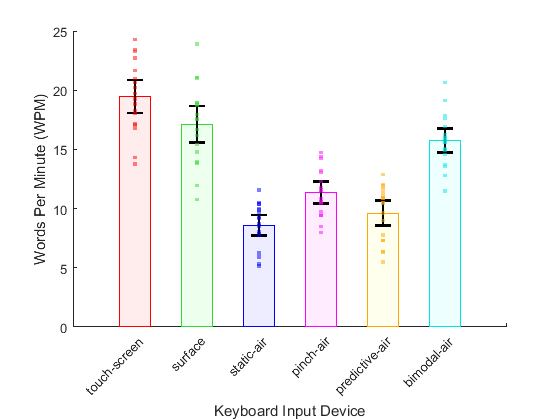
\includegraphics{Figures/fig_textentry_mean}
	\caption[Mean Text-entry Rates]{Mean Text-entry Rates for each keyboard with error bars showing 95\% confidence intervals.}
	\label{fig_textentry_mean}
\end{figure}

The multiple comparisons, seen in Table~\ref{textentry_multcompare}, revealed significant differences ($p$-values $<$ 0.001) in text-entry rates between the Touch Screen Keyboard and all mid-air keyboards. There were significant differences ($p$-values $<$ 0.0001) between the Leap Surface Keyboard and the Static-air, Pinch-air, and Predictive-air keyboards. There were also significant differences ($p$-values $<$ 0.0001) found between the Leap Bimodal-air and all other mid-air keyboards. Finally, there was a significant difference ($p$-value = 0.0170) found between the Pinch-air and Static-air keyboards.

Unfortunately, no mid-air keyboards were able to achieve text-entry rates as fast as the Touch Screen Keyboard and were significantly slower. However, the Bimodal-air keyboard reached a mean text-entry rate of 15.8 WPM without repeated sessions or training, indicating promising results. With repeated sessions, as in Vulture \cite{ref_vulture}, the Bimodal Keyboard is expected to increase in performance by approximately 75\%. The increase is expected to be even greater (approximately 238\%) when training for single short phrases, reaching speeds sufficiently high enough to compete with touch-based keyboards and surpass pinching as a means of mid-air word-gesturing.

Both the Static-air and Predictive-air keyboards underperformed, though the Predictive-air keyboard achieved marginally better results. These results were expected since adding the 3rd-dimension as a means of interaction further increased keyboard complexity and the mental coupling required between gestures in the motor-space and feedback on the display \cite{ref_vulture,ref_stimulus_response_compatibility}. It was interesting to see how well the Leap Surface Keyboard performed since it had an identical implementation as the Leap Static-air Keyboard, only differing in where the interaction plane was projected. This implies that visually representing the Leap Static-air keyboard in 3-dimensional space using augmented reality might have the same results due to the decreased decoupling between the motor space and display space.

\subsection{Text-entry Rate Modified-shortest}
Participants reached a mean text-entry rate of 19.7 WPM ($SD = 2.9$) for the Touch Screen Keyboard, 17.3 WPM ($SD = 3.3$) for the Leap Surface Keyboard, 8.8 WPM ($SD = 1.9$) for the Leap Static-air Keyboard, 11.6 WPM ($SD = 2.1$) for the Leap Pinch-air Keyboard, 9.9 WPM ($SD = 2.3$) for the Predictive-air Keyboard, and 15.9 WPM ($SD = 2.2$) for the Leap Bimodal-air Keyboard. Figure~\ref{fig_textentry_short_mean} shows the mean text-entry rates for each keyboard interaction style using the shortest-transcribed modification. Using a one-way ANOVA, a significant difference was detected between keyboard means ($F(5, 102) = 54.6430$, $p$-value $<$ 0.0001, $SD_{pooled} = 2.5$), prompting the use of Tukey's HSD with multiple-compare for further analysis.

\begin{figure}[!t]
	\centering
	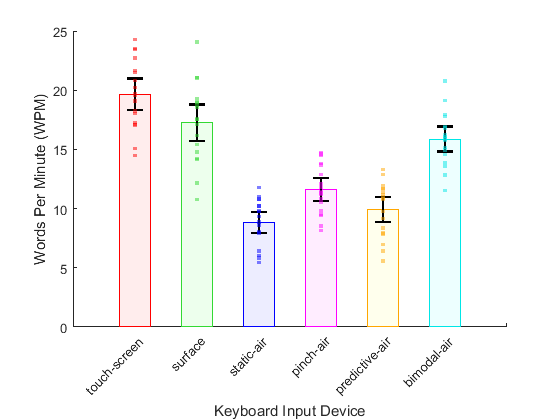
\includegraphics{Figures/fig_textentry_short_mean}
	\caption[Mean Text-entry Rates for Modified-shortest]{Mean Text-entry Rates using the shortest-transcribed modification for each keyboard with error bars showing 95\% confidence intervals.}
	\label{fig_textentry_short_mean}
\end{figure}

The multiple comparisons, seen in Table~\ref{textentry_short_multcompare}, revealed significant differences ($p$-values $<$ 0.001) in text-entry rates between the Touch Screen Keyboard and all mid-air keyboards. There were significant differences ($p$-values $<$ 0.0001) between the Leap Surface Keyboard and the Static-air, Pinch-air, and Predictive-air keyboards. There were also significant differences ($p$-values $<$ 0.0001) found between the Leap Bimodal-air and all other mid-air keyboards. The highest Bimodal-air text-entry rates were on par with the Touch Screen Keyboard. Finally, there was a significant difference ($p$-value = 0.0148) found between the Pinch-air and Static-air keyboards.

The results from using the shortest-transcribed modification were marginally better than those without, implying that errors were more likely corrected while gesturing the words rather than after having completed the gesture. The cases where errors were made while still entering all required letters seem to have had very little impact on the duration it took to complete words.

\section{Error Rate}

\subsection{Minimum Word Distance}
Participants reached a mean MWD of 13.0\% ($SD = 13.4$) for the Touch Screen Keyboard, 18.9\% ($SD = 14.0$) for the Leap Surface Keyboard, 56.7\% ($SD = 19.4$) for the Leap Static-air Keyboard, 34.4\% ($SD = 19.4$) for the Leap Pinch-air Keyboard, 48.9\% ($SD = 25.2$) for the Predictive-air Keyboard, and 20.4\% ($SD = 16.9$) for the Leap Bimodal-air Keyboard. Figure~\ref{fig_MWD_mean} shows the mean Minimum Word Distance for each keyboard interaction style. Using a one-way ANOVA, a significant difference was detected between keyboard means ($F(5, 102) = 16.5496$, $p$-value $<$ 0.0001, $SD_{pooled} = 18.5$), prompting the use of Tukey's HSD with multiple-compare for further analysis.

\begin{figure}[!t]
	\centering
	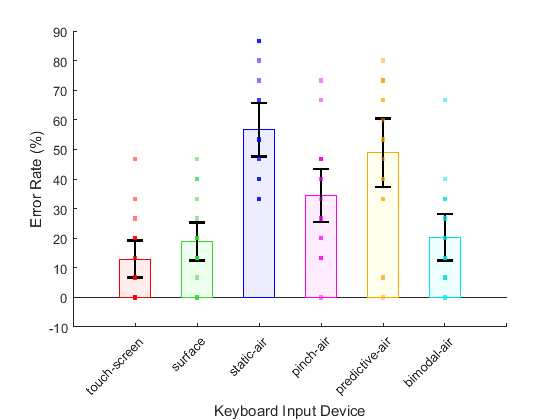
\includegraphics{Figures/fig_MWD_mean}
	\caption[Mean Minimum Word Distance]{Mean Minimum Word Distance for each keyboard with error bars showing 95\% confidence intervals.}
	\label{fig_MWD_mean}
\end{figure}

The multiple comparisons, seen in Table~\ref{MWD_multcompare}, revealed significant differences ($p$-values $<$ 0.01) in Minimum Word Distance between the Touch Screen Keyboard and the Leap Static-air, Pinch-air, and Predictive-air keyboards. There were significant differences ($p$-values $<$ 0.0001) between the Leap Surface Keyboard and the Static-air and Predictive-air keyboards. There were also significant differences ($p$-values $<$ 0.001) found between the Leap Bimodal-air and the Static-air and Predictive-air keyboards. There was finally a significant difference ($p$-value = 0.0062) found between the Leap Pinch-air and Static-air keyboards.

The error rates here were much higher than those seen in Vulture for Pinch or Touch \cite{ref_vulture} because this was a modified version of MWD. Since participants were required to fix errors, the MWD from Vulture would have seen error rates of 0\%. Instead, if any errors were detected during the typing process, whether it be from device detection issues or the participant going for the wrong letter, the word was counted as erroneous. This representation of MWD showed how many words needed correcting for any reason.

The Static-air and Predictive-air keyboards underperformed, as expected, due to the increased decoupling and the added complexity of working with the 3rd-dimension. The Leap Bimodal-air Keyboard was significantly less erroneous than the Static-air and Predictive-air keyboards and was not significantly different from the Touch Screen Keyboard, implying that removing the 3rd-dimension significantly reduces the effects of decoupling on hand-eye coordination efforts. Again, the Leap Surface was on par with the Touch Screen keyboard, suggesting that with augmented reality the Static-air Keyboard could see a significant improvement in performance in all areas.

\subsubsection{MWD modified-shortest}
Participants reached a mean MWD of 6.3\% ($SD = 9.0$) for the Touch Screen Keyboard, 6.3\% ($SD = 6.3$) for the Leap Surface Keyboard, 25.6\% ($SD = 20.7$) for the Leap Static-air Keyboard, 20.0\% ($SD = 11.2$) for the Leap Pinch-air Keyboard, 26.0\% ($SD = 16.6$) for the Predictive-air Keyboard, and 10.0\% ($SD = 11.7$) for the Leap Bimodal-air Keyboard. Figure~\ref{fig_MWD_short_mean} shows the mean Minimum Word Distance with the shortest-transcribed modification for each keyboard interaction style. Using a one-way ANOVA, a significant difference was detected between keyboard means ($F(5, 102) = 8.5172$, $p$-value $<$ 0.0001, $SD_{pooled} = 13.5$), prompting the use of Tukey's HSD with multiple-compare for further analysis.

\begin{figure}[!t]
	\centering
	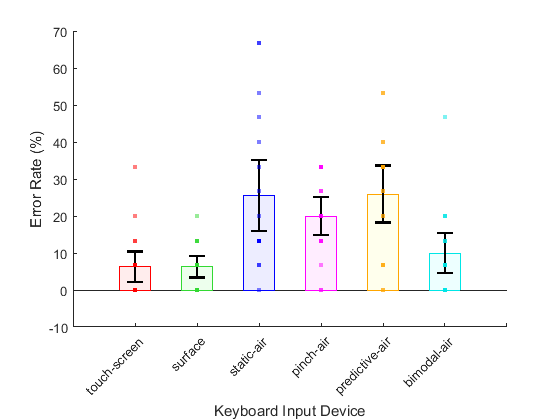
\includegraphics{Figures/fig_MWD_short_mean}
	\caption[Mean Minimum Word Distance for Modified-shortest]{Mean Minimum Word Distance using the shortest-transcribed modification for each keyboard with error bars showing 95\% confidence intervals.}
	\label{fig_MWD_short_mean}
\end{figure}

The multiple comparisons, seen in Table~\ref{MWD_short_multcompare}, revealed significant differences ($p$-values $<$ 0.05) in Minimum Word Distance with the shortest-transcribed modification between the Touch Screen Keyboard and the Leap Static-air, Pinch-air, and Predictive-air keyboards. There were significant differences ($p$-values $<$ 0.05) between the Leap Surface Keyboard and the Leap Static-air, Pinch-air, and Predictive-air keyboards. There were also significant differences ($p$-values $<$ 0.01) found between the Leap Bimodal-air and the Static-air and Predictive-air keyboards.

The substantial reductions in MWD error rates when using the shortest-transcribed modification, nearly 50\% reduction for all keyboards, indicated that many participants seemed to be making errors after entering all of the required letters for a gestured word. This may imply situations like Example 4 from Table~\ref{shortest_transcribed}, where participants were typing the wrong word, such as ``fired'' compared to ``fire''. However, for all Leap Motion-based keyboards, the more likely implication is that many participants made errors on exiting the interaction plane. This kind of error was observed often and was thought to be heavily influenced by participants pulling their hands away from the interaction plane in an arcing motion, especially for participants who were resting their arms. Figure~\ref{arcing_motion} details this arcing motion. It is expected that a word-recognition implementation of the word-gesture keyboards would see even lower error rates closer to those found in Vulture \cite{ref_vulture}, implying that the pseudo-implementation of the word-gesture keyboards was less robust and more sensitive to deviations in a word's gesture-shape than traditional word-gesture keyboards implemented with word-recognition.

\begin{figure}[!t]
	\centering
	\begin{minipage}[t]{2.5in}
		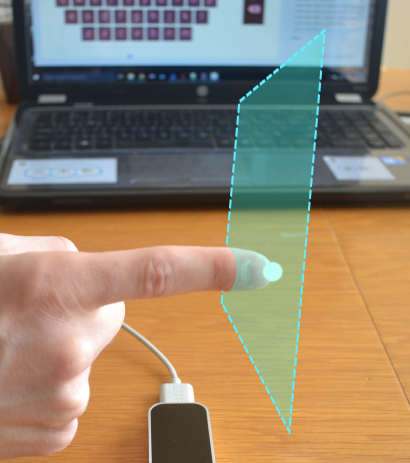
\includegraphics[width=2.5in]{Figures/fig_arc_down}
		\subcaption{Pressing Final Key}
	\end{minipage}
	\begin{minipage}[t]{2.5in}
		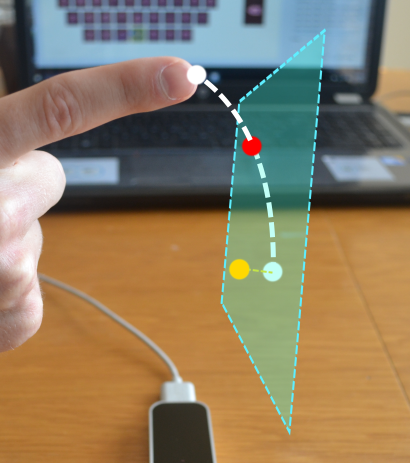
\includegraphics[width=2.5in]{Figures/fig_arc_up}
		\subcaption{Removing Hand From Plane}
	\end{minipage}
	\caption[Arcing Motion]{Examples of how the natural arcing motion generates erroneous input for 3-dimensional interactions. (a) shows the user pressing the final key; and (b) shows the intended release in \textit{yellow} and the detected release in \textit{red}.}
	\label{arcing_motion}
\end{figure}

\subsection{Keystrokes Per Character}
Participants reached a mean KSPC of 1.2 keystrokes per character ($SD = 0.18$) for the Touch Screen Keyboard, 1.4 keystrokes per character  ($SD = 0.38$) for the Leap Surface Keyboard, 2.0 keystrokes per character ($SD = 0.79$) for the Leap Static-air Keyboard, 1.6 keystrokes per character ($SD = 0.42$) for the Leap Pinch-air Keyboard, 1.9 keystrokes per character ($SD = 0.64$) for the Predictive-air Keyboard, and 1.2 keystrokes per character ($SD = 0.18$) for the Leap Bimodal-air Keyboard. Figure~\ref{fig_KSPC_mean} shows the mean Keystrokes Per Character for each keyboard interaction style. Using a one-way ANOVA, a significant difference was detected between keyboard means ($F(5, 102) = 9.8827$, $p$-value $<$ 0.0001, $SD_{pooled} = 0.49$), prompting the use of Tukey's HSD with multiple-compare for further analysis.

\begin{figure}[!t]
	\centering
	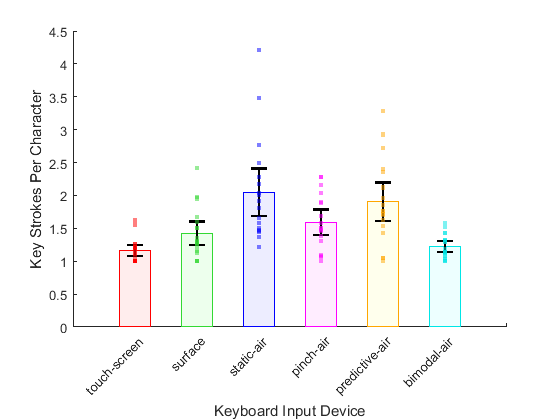
\includegraphics{Figures/fig_KSPC_mean}
	\caption[Mean Keystrokes Per Character]{Mean Keystrokes Per Character for each keyboard with error bars showing 95\% confidence intervals.}
	\label{fig_KSPC_mean}
\end{figure}

The multiple comparisons, seen in Table~\ref{KSPC_multcompare}, revealed significant differences ($p$-values $<$ 0.001) in Keystrokes Per Character between the Touch Screen Keyboard and the Leap Static-air and Predictive-air keyboards. There were significant differences ($p$-values $<$ 0.05) between the Leap Surface Keyboard and the Static-air and Predictive-air keyboards. There were also significant differences ($p$-values $<$ 0.01) found between the Leap Bimodal-air and the Static-air and Predictive-air keyboards.

Keystrokes Per Character was useful when analyzing the pseudo implementation of the word-gesture keyboards because words were constructed at the character level, rather than at the word level as with word-recognition. With KSPC, if words were input without any detected errors, then a KSPC of 1.0 keystrokes would be expected. This metric helps show the rate at which extra erroneous characters were produced for each keyboard. For example, the KSPC of the Static-air keyboard was 2.0 keystrokes, meaning 100\% more interactions were produced than required to gesture the words successfully. As before, the Static-air and Predictive-air keyboard performances were underwhelming, and the Bimodal-air performed on par with the Touch Screen and Leap Surface keyboards. The Pinch-air performed somewhere in between the other Leap Motion-based keyboards. As these means continue to show, a trend was developing in the dependent measures between the keyboards and was expected to hold for all other variables.

\subsubsection{KSPC modified-shortest}
Participants reached a mean KSPC of 1.1 keystrokes per character ($SD = 0.14$) for the Touch Screen Keyboard, 1.3 keystrokes per character ($SD = 0.27$) for the Leap Surface Keyboard, 1.7 keystrokes per character ($SD = 0.48$) for the Leap Static-air Keyboard, 1.4 keystrokes per character ($SD = 0.31$) for the Leap Pinch-air Keyboard, 1.7 keystrokes per character ($SD = 0.43$) for the Predictive-air Keyboard, and 1.1 keystrokes per character ($SD = 0.15$) for the Leap Bimodal-air Keyboard. Figure~\ref{fig_KSPC_short_mean} shows the mean Keystrokes Per Character with the shortest-transcribed modification for each keyboard interaction style. Using a one-way ANOVA, a significant difference was detected between keyboard means ($F(5, 102) = 11.5949$, $p$-value $<$ 0.0001, $SD_{pooled} = 0.32$), prompting the use of Tukey's HSD with multiple-compare for further analysis.

\begin{figure}[!t]
	\centering
	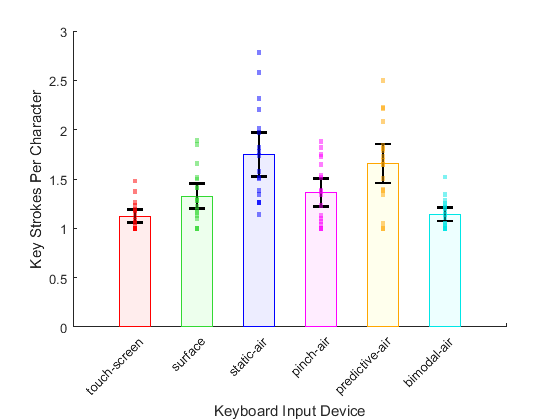
\includegraphics{Figures/fig_KSPC_short_mean}
	\caption[Mean Keystrokes Per Character for Modified-shortest]{Mean Keystrokes Per Character using the shortest-transcribed modification for each keyboard with error bars showing 95\% confidence intervals.}
	\label{fig_KSPC_short_mean}
\end{figure}

The multiple comparisons, seen in Table~\ref{KSPC_short_multcompare}, revealed significant differences ($p$-values $<$ 0.0001) in Keystrokes Per Character with the shortest-transcribed modification between the Touch Screen Keyboard and the Leap Static-air and Predictive-air keyboards. There were significant differences ($p$-values $<$ 0.05) between the Leap Surface Keyboard and the Leap Static-air and Predictive-air keyboards. There were also significant differences ($p$-values $<$ 0.001) found between the Leap Bimodal-air Keyboard and the Static-air and Predictive-air keyboards. Finally there was a significant difference ($p$-value = 0.0072) between the Pinch-air and Static-air keyboards.

As with MWD, KSPC saw huge improvements with the shortest-transcribed modification, especially for Leap Motion-based keyboards. This reaffirmed that a large number of errors were produced during exiting the interaction plane.

\subsection{Minimum String Distance}

\subsubsection{MSD modified-shortest}
Participants reached a mean MSD of 1.6\% ($SD = 2.4$) for the Touch Screen Keyboard, 2.2\% ($SD = 2.4$) for the Leap Surface Keyboard, 6.4\% ($SD = 5.0$) for the Leap Static-air Keyboard, 5.1\% ($SD = 3.1$) for the Leap Pinch-air Keyboard, 5.4\% ($SD = 3.3$) for the Predictive-air Keyboard, and 2.5\% ($SD = 2.6$) for the Leap Bimodal-air Keyboard. Figure~\ref{fig_MSD_short_mean} shows the mean Minimum String Distance with the shortest-transcribed modification for each keyboard interaction style. Using a one-way ANOVA, a significant difference was detected between keyboard means ($F(5, 102) = 6.8688$, $p$-value $<$ 0.0001, $SD_{pooled} = 3.3$), prompting the use of Tukey's HSD with multiple-compare for further analysis.

\begin{figure}[!t]
	\centering
	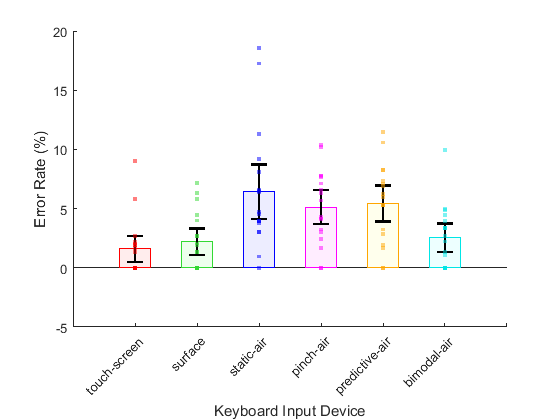
\includegraphics{Figures/fig_MSD_short_mean}
	\caption[Mean Minimum String Distance for Modified-shortest]{Mean Minimum String Distance using the shortest-transcribed modification for each keyboard with error bars showing 95\% confidence intervals.}
	\label{fig_MSD_short_mean}
\end{figure}

The multiple comparisons, seen in Table~\ref{MSD_short_multcompare}, revealed significant differences ($p$-values $<$ 0.05) in Minimum String Distance with the shortest-transcribed modification between the Touch Screen Keyboard and the Leap Static-air, Pinch-air, and Predictive-air keyboards. There were significant differences ($p$-values $<$ 0.05) between the Leap Surface Keyboard and the Leap Static-air and Predictive-air keyboards both. There was also a significant difference ($p$-value $=$ 0.0067) found between the Leap Bimodal-air and the Static-air keyboards.

The error rates seen for the Pinch-air and Touch Screen keyboards for MSD with the shortest-transcribed modification were similar to those found in Vulture for their MWD \cite{ref_vulture}. It is expected that with practice or repeated sessions, these error rates would become even less. The keyboards again follow the same pattern as other measures, providing more evidence of the effects of decoupling on performance and complexity when using 3-dimensions versus a tangible surface. Notably, the Leap Bimodal-air seems to be mostly unaffected by decoupling between the motor space and display space and seems to be only minimally affected by complexity, only having been significantly different from the Touch Screen Keyboard for text-entry rates.

\subsection{Total Error Rate}
Participants reached a mean Total Error Rate of 4.9\% ($SD = 5.5$) for the Touch Screen Keyboard, 9.3\% ($SD = 7.1$) for the Leap Surface Keyboard, 23.6\% ($SD = 12.1$) for the Leap Static-air Keyboard, 14.1\% ($SD = 9.0$) for the Leap Pinch-air Keyboard, 20.1\% ($SD = 11.4$) for the Predictive-air Keyboard, and 6.8\% ($SD = 5.5$) for the Leap Bimodal-air Keyboard. Figure~\ref{fig_totER_mean} shows the mean Total Error Rate for each keyboard interaction style. Using a one-way ANOVA, a significant difference was detected between keyboard means ($F(5, 102) = 12.9381$, $p$-value $<$ 0.0001, $SD_{pooled} = 8.8$), prompting the use of Tukey's HSD with multiple-compare for further analysis.

\begin{figure}[!t]
	\centering
	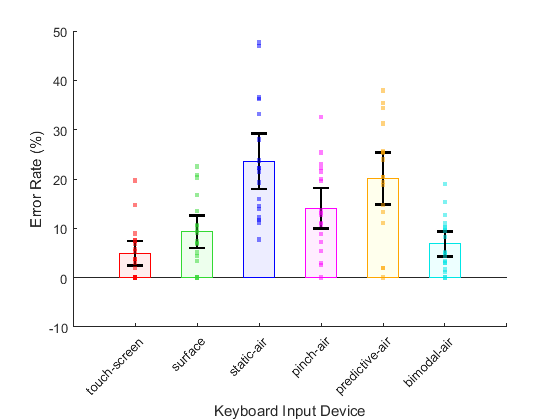
\includegraphics{Figures/fig_totER_mean}
	\caption[Mean Total Error Rates]{Mean Total Error Rates for each keyboard with error bars showing 95\% confidence intervals.}
	\label{fig_totER_mean}
\end{figure}

The multiple comparisons, seen in Table~\ref{totER_multcompare}, revealed significant differences ($p$-values $<$ 0.0001) in Total Error Rate between the Touch Screen Keyboard and the Leap Static-air and Predictive-air keyboards. There were significant differences ($p$-values $<$ 0.01) between the Leap Surface Keyboard and the Static-air and Predictive-air keyboards. There were also significant differences ($p$-values $<$ 0.01) found between the Leap Bimodal-air and the Static-air and Predictive-air keyboards. Finally, there was a significant difference ($p$-value = 0.0191) between the Pinch-air and the Static-air keyboards.

Again, the keyboards follow the same pattern. The Bimodal-air and Leap Surface keyboards perform approximately as well as the Touch Screen Keyboard while the Static-air and Predictive-air keyboards continue to fall short. The Pinch-air keyboard falls somewhere in the middle for Total Error Rate, showing no significant differences with any keyboards.

\subsubsection{Total error rate modified-shortest}
Participants reached a mean Total Error Rate of 4.9\% ($SD = 5.4$) for the Touch Screen Keyboard, 9.2\% ($SD = 7.0$) for the Leap Surface Keyboard, 23.3\% ($SD = 11.8$) for the Leap Static-air Keyboard, 13.5\% ($SD = 8.9$) for the Leap Pinch-air Keyboard, 19.4\% ($SD = 10.7$) for the Predictive-air Keyboard, and 6.7\% ($SD = 5.3$) for the Leap Bimodal-air Keyboard. Figure~\ref{fig_totER_short_mean} shows the mean Total Error Rate with the shortest-transcribed modification for each keyboard interaction style. Using a one-way ANOVA, a significant difference was detected between keyboard means ($F(5, 102) = 13.0717$, $p$-value $<$ 0.0001, $SD_{pooled} = 8.6$), prompting the use of Tukey's HSD with multiple-compare for further analysis.

\begin{figure}[!b]
	\centering
	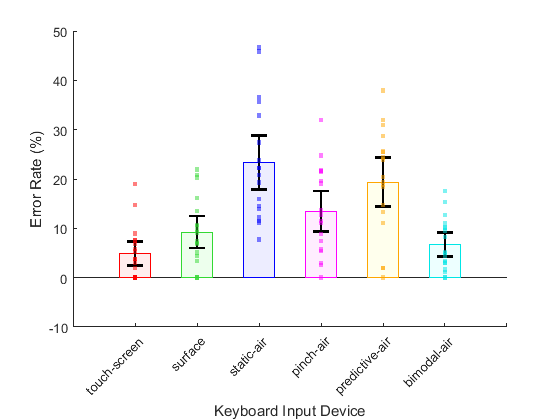
\includegraphics{Figures/fig_totER_short_mean}
	\caption[Mean Total Error Rate for Modified-shortest]{Mean Total Error Rate using the shortest-transcribed modification for each keyboard with error bars showing 95\% confidence intervals.}
	\label{fig_totER_short_mean}
\end{figure}

The multiple comparisons, seen in Table~\ref{totER_short_multcompare}, revealed significant differences ($p$-values $<$ 0.05) in Total Error Rate with the shortest-transcribed modification between the Touch Screen Keyboard and the Leap Static-air, Pinch-air, and Predictive-air keyboards. There were significant differences ($p$-values $<$ 0.01) between the Leap Surface Keyboard and the Leap Static-air and Predictive-air keyboards. There were also significant differences found between the Leap Bimodal-air and the Static-air and Predictive-air keyboards with a $p$-value $<$ 0.001. Finally, there was a significant difference ($p$-value = 0.0101) between the Pinch-air and Static-air keyboards.

Surprisingly, unlike KSPC and MWD, the Total Error Rate did not follow suit by showing large decreases in error rate with the shortest-transcribed modification. However, these observations continue to support the findings between the text-entry rates with and without modification, which were also relatively unaffected by the shortest-transcribed modification. This further implied that errors made by participants were more likely corrected throughout gesturing words rather than after having completed the word-gesture. This was a major downside of lacking word-recognition because gestures were interrupted and corrected rather than being completed with errors, as is natural to traditional word-gesture keyboards.

\section{Correctness}
\subsection{Fr\'echet Distance} \label{results_frechet}
Participants reached a mean Fr\'echet Distance of 231.2 pixels ($SD = 26.7$) for the Touch Screen Keyboard, 242.8 pixels ($SD = 30.4$) for the Leap Surface Keyboard, 364.3 pixels ($SD = 86.5$) for the Leap Static-air Keyboard, 501.2 pixels ($SD = 42.8$) for the Leap Pinch-air Keyboard, 350.6 pixels ($SD = 86.8$) for the Predictive-air Keyboard, and 396.5 pixels ($SD = 102.1$) for the Leap Bimodal-air Keyboard. Figure~\ref{fig_frechet_mean} shows the mean Fr\'echet Distance for each keyboard interaction style. Using a one-way ANOVA, a significant difference was detected between keyboard means ($F(5, 102) = 37.9416$, $p$-value $<$ 0.0001, $SD_{pooled} = 69.4$), prompting the use of Tukey's HSD with multiple-compare for further analysis.

\begin{figure}[!t]
	\centering
	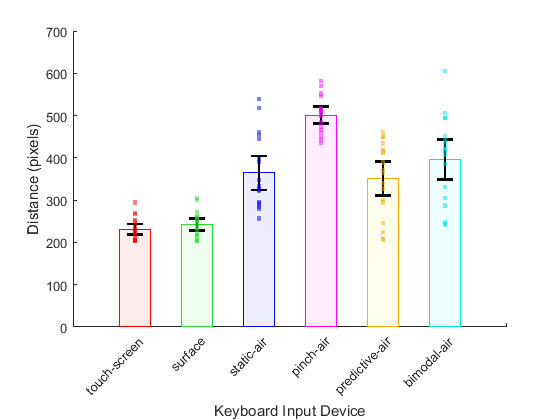
\includegraphics{Figures/fig_frechet_mean}
	\caption[Mean Fr\'echet Distance]{Mean Fr\'echet Distance for each keyboard with error bars showing 95\% confidence intervals.}
	\label{fig_frechet_mean}
\end{figure}

The multiple comparisons, seen in Table~\ref{frechet_multcompare}, revealed significant differences ($p$-values $<$ 0.0001) in Fr\'echet Distance between the Touch Screen Keyboard and all of the mid-air keyboards. There were significant differences ($p$-values $<$ 0.001) between the Leap Surface Keyboard and all of the mid-air keyboards. There were also significant differences ($p$-values $<$ 0.001) found between the Leap Pinch-air and all of the other mid-air keyboards.

The Fr\'echet Distance was the only place where the trends were broken and the Bimodal-air keyboard performed significantly worse than the Touch Screen and Leap Surface keyboards. The Pinch-air Keyboard also performed significantly worse than all other keyboards. These results were assumed to be caused by a combination of the word-gesture velocity seen in Section~\ref{results_velocity_gesture} and the effects of either increased decoupling or complexity from working with the 3rd-dimension. Appendix~\ref{user_generated_paths} emphasizes these assumptions by illustrating the participant-generated word-gesture paths for all word sets and their corresponding keyboards.

The Leap Bimodal-air seemed to suffer in correctness due to its very high word-gesture velocities, whereas the Static-air and Predictive-air benefit in correctness due to their very slow word-gesture velocities. Participants used explicitly slower, more precise gestures to compensate for these keyboards' increased decoupling. The Leap Surface and Touch Screen keyboards were relatively unaffected in correctness by their high word-gesturing velocities due to their decreased decoupling of the word-gesture motor space from the displayed screen.

The Pinch-air Keyboard suffered from the combination of high word-gesture velocities and effects of increased decoupling. However, the Pinch-air Keyboard also seemed to be heavily affected by the deviation in its tracking method, which increased the overall distance traveled for each word-gesture, as seen in Section~\ref{results_distance}. All other mid-air keyboards tracked participants' pointer fingers, whereas the Pinch-air keyboard tracked participants' palms. Palms were tracked instead because participants' fingers moved drastically when creating a pinching gesture. This difference in tracking combined with high word-gesture velocities were the assumed factors for this decrease in performance.

\subsubsection{Fr\'echet distance modified-shortest}
Participants reached a mean Fr\'echet Distance of 221.0 pixels ($SD = 18.0$) for the Touch Screen Keyboard, 231.0 pixels ($SD = 22.7$) for the Leap Surface Keyboard, 306.4 pixels ($SD = 53.2$) for the Leap Static-air Keyboard, 459.2 pixels ($SD = 20.1$) for the Leap Pinch-air Keyboard, 281.6 pixels ($SD = 49.9$) for the Predictive-air Keyboard, and 368.4 pixels ($SD = 82.4$) for the Leap Bimodal-air Keyboard. Figure~\ref{fig_frechet_short_mean} shows the mean Fr\'echet Distance with the shortest-transcribed modification for each keyboard interaction style. Using a one-way ANOVA, a significant difference was detected between keyboard means ($F(5, 102) = 65.7440$, $p$-value $<$ 0.0001, $SD_{pooled} = 47.2$), prompting the use of Tukey's HSD with multiple-compare for further analysis.

\begin{figure}[!t]
	\centering
	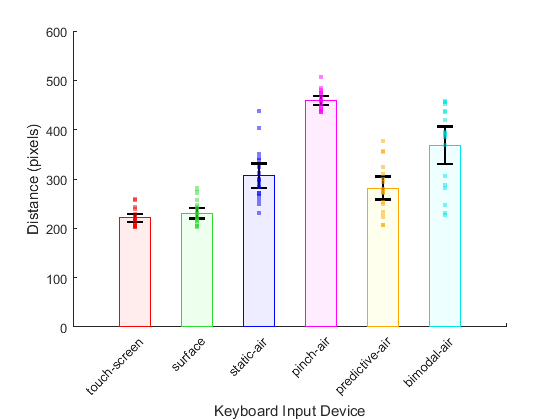
\includegraphics{Figures/fig_frechet_short_mean}
	\caption[Mean Fr\'echet Distance for Modified-shortest]{Mean Fr\'echet Distance using the shortest-transcribed modification for each keyboard with error bars showing 95\% confidence intervals.}
	\label{fig_frechet_short_mean}
\end{figure}

The multiple comparisons, seen in Table~\ref{frechet_short_multcompare}, revealed significant differences ($p$-values $<$ 0.01) in Fr\'echet Distance with the shortest-transcribed modification between the Touch Screen Keyboard and all of the mid-air keyboards. There were significant differences ($p$-values $<$ 0.05) between the Leap Surface Keyboard and all of the mid-air keyboards. There were also significant differences ($p$-values $<$ 0.01) found between the Leap Bimodal-air Keyboard and the other mid-air keyboards. Finally, there were significant differences ($p$-values $<$ 0.0001) found between the Leap Pinch-air Keyboard and the Static-air and Predictive-air keyboards.

The increased correctness for all keyboards, especially the mid-air keyboards, when using the shortest-transcribed modification implies that many errors were being produced when exiting the interaction plane. This was especially evident for the Static-air, Pinch-air, and Predictive-air keyboards, which all saw the largest improvements to correctness. For the Static-air and Predictive-air keyboards, these errors were caused by the addition of the 3rd-dimension and participants having trouble entering and exiting the interaction plane accurately. The Pinch-air Keyboard saw a combination of high word-gesture velocity and a different method of tracking that was assumed to produce these kinds of errors.

\subsubsection{Fr\'echet distance modified-backspace}
Participants reached a mean Fr\'echet Distance of 212.3 pixels ($SD = 9.3$) for the Touch Screen Keyboard, 223.5 pixels ($SD = 18.5$) for the Leap Surface Keyboard, 258.9 pixels ($SD = 33.5$) for the Leap Static-air Keyboard, 444.7 pixels ($SD = 8.0$) for the Leap Pinch-air Keyboard, 237.7 pixels ($SD = 24.8$) for the Predictive-air Keyboard, and 356.8 pixels ($SD = 85.0$) for the Leap Bimodal-air Keyboard. Figure~\ref{fig_frechet_back_mean} shows the mean Fr\'echet Distance with the backspace-transcribed modification for each keyboard interaction style. Using a one-way ANOVA, a significant difference was detected between keyboard means ($F(5, 102) = 97.1196$, $p$-value $<$ 0.0001, $SD_{pooled} = 39.7$), prompting the use of Tukey's HSD with multiple-compare for further analysis.

\begin{figure}[!t]
	\centering
	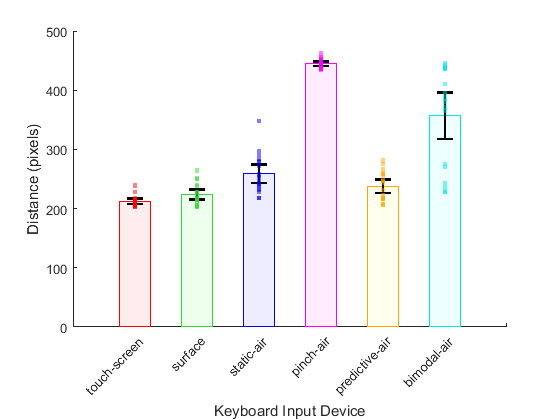
\includegraphics{Figures/fig_frechet_back_mean}
	\caption[Mean Fr\'echet Distance for Modified-backspace]{Mean Fr\'echet Distance using the backspace-transcribed modification for each keyboard with error bars showing 95\% confidence intervals.}
	\label{fig_frechet_back_mean}
\end{figure}

The multiple comparisons, seen in Table~\ref{frechet_back_multcompare}, revealed significant differences ($p$-values $<$ 0.01) in Fr\'echet Distance with the backspace-transcribed modification between the Touch Screen Keyboard and the Leap Static-air, Pinch-air, and Bimodal-air keyboards. There were significant differences ($p$-values $<$ 0.0001) between the Leap Surface Keyboard and the Leap Pinch-air and Bimodal-air keyboards. There were also significant differences ($p$-values $<$ 0.0001) found between the Leap Bimodal-air and all other mid-air keyboards. Finally, there were significant differences ($p$-values $<$ 0.0001) between the Leap Pinch-air Keyboard and the Static-air and Predictive-air keyboards.

If the backspace key was included in the path considered to be correct for Fr\'echet Distance, since participants were required to correct words, a boost in correctness was observed. The Bimodal-air and Pinch-air keyboards still suffered from the previously mentioned problems in Section~\ref{results_frechet}. The Static-air and Predictive-air, however, saw huge improvements in correctness because of the low word-gesture velocities and high error rates. The Predictive-air Keyboard, in this case, was not significantly different from the Touch Screen and Leap Surface keyboards, implying that participants were relatively attentive to correcting errors for it.

\section{Distance Measures}
\subsection{Word-gesture Distance} \label{results_distance}
Participants reached a mean Word-gesture Distance of 1087.5 pixels ($SD = 85.9$) for the Touch Screen Keyboard, 1423.9 pixels ($SD = 246.0$) for the Leap Surface Keyboard, 1590.9 pixels ($SD = 508.2$) for the Leap Static-air Keyboard, 2165.3 pixels ($SD = 540.5$) for the Leap Pinch-air Keyboard, 1634.7 pixels ($SD = 481.4$) for the Predictive-air Keyboard, and 1627.7 pixels ($SD = 321.3$) for the Leap Bimodal-air Keyboard. Figure~\ref{fig_distance_mean} shows the mean Word-gesture Distance for each keyboard interaction style. Using a one-way ANOVA, a significant difference was detected between keyboard means ($F(5, 102) = 13.9225$, $p$-value $<$ 0.0001, $SD_{pooled} = 398.6$), prompting the use of Tukey's HSD with multiple-compare for further analysis.

\begin{figure}[!t]
	\centering
	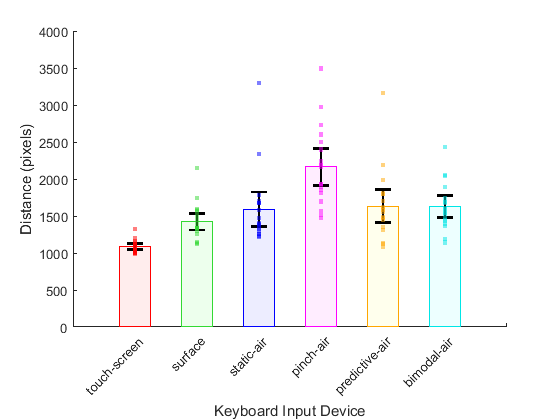
\includegraphics{Figures/fig_distance_mean}
	\caption[Mean Word-gesture Distance]{Mean Word-gesture Distance for each keyboard with error bars showing 95\% confidence intervals.}
	\label{fig_distance_mean}
\end{figure}

The multiple comparisons, seen in Table~\ref{distance_multcompare}, revealed significant differences ($p$-values $<$ 0.01) in Word-gesture Distance between the Touch Screen Keyboard and all of the mid-air keyboards. There were also significant differences ($p$-values $<$ 0.01) between the Leap Pinch-air and all other Leap Motion-based keyboards.

As expected, all mid-air keyboards required longer word-gesture distances than the Touch Screen Keyboard due to the effect of decoupling between the word-gesture motor space and the keyboard display. It was surprising, however, that the Leap Surface Keyboard required significantly more word-gesture distance than the Touch Screen Keyboard. This could be because of the requirement to use a stylus rather than the participants' bare hands.

The Pinch-air keyboard required a significantly longer word-gesture distance than all other keyboards. This was assumed to be caused by the different tracking method as previously mentioned. Tracking the palm required broader, less controlled movements than tracking fingers or a stylus.

\subsubsection{Word-gesture distance modified-shortest}
Participants reached a mean Word-gesture Distance of 1081.3 ($SD = 84.6$) for the Touch Screen Keyboard, 1396.5 ($SD = 226.5$) for the Leap Surface Keyboard, 1524.8 ($SD = 412.5$) for the Leap Static-air Keyboard, 1981.4 ($SD = 470.6$) for the Leap Pinch-air Keyboard, 1536.7 ($SD = 346.1$) for the Predictive-air Keyboard, and 1566.5 ($SD = 253.6$) for the Leap Bimodal-air Keyboard. Figure~\ref{fig_distance_short_mean} shows the mean Word-gesture Distance with the shortest-transcribed modification for each keyboard interaction style. Using a one-way ANOVA, a significant difference was detected between keyboard means ($F(5, 102) = 14.403$, $p$-value $<$ 0.0001, $SD_{pooled} = 325.1$), prompting the use of Tukey's HSD with multiple-compare for further analysis.

\begin{figure}[!t]
	\centering
	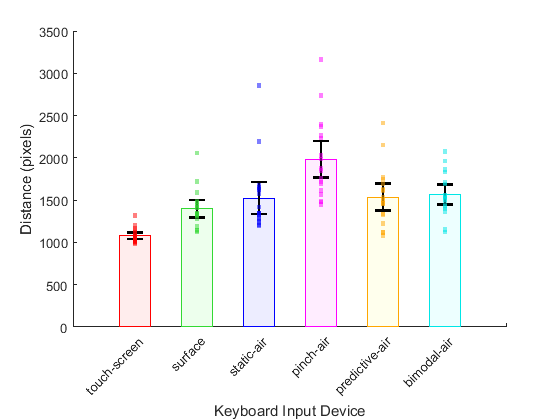
\includegraphics{Figures/fig_distance_short_mean}
	\caption[Mean Word-gesture Distance for Modified-shortest]{Mean Word-gesture Distance using the shortest-transcribed modification for each keyboard with error bars showing 95\% confidence intervals.}
	\label{fig_distance_short_mean}
\end{figure}

The multiple comparisons, seen in Table~\ref{distance_short_multcompare}, revealed significant differences ($p$-values $<$ 0.05) in Word-gesture Distance with the shortest-transcribed modification between the Touch Screen Keyboard and all other keyboards. There were significant differences ($p$-values $<$ 0.01) between the Leap Surface and Pinch-air keyboards and all other Leap Motion-based keyboards.

Again, the small difference between the word-gesture distance and the word-gesture distance using the shortest-transcribed modification implied that most errors were corrected by participants while in the middle of typing words.

\subsection{Word-gesture Velocity} \label{results_velocity_gesture}
Participants reached a mean Word-gesture Velocity of 673.3 $pixels/s$ ($SD = 126.4$) for the Touch Screen Keyboard, 641.1 $pixels/s$ ($SD = 165.5$) for the Leap Surface Keyboard, 380.9 $pixels/s$ ($SD = 78.2$) for the Leap Static-air Keyboard, 643.8 $pixels/s$ ($SD = 204.7$) for the Leap Pinch-air Keyboard, 405.6 $pixels/s$ ($SD = 87.6$) for the Predictive-air Keyboard, and 777.6 $pixels/s$ ($SD = 240.9$) for the Leap Bimodal-air Keyboard. Figure~\ref{fig_velocity_gesture_mean} shows the mean Word-gesture Velocity for each keyboard interaction style. Using a one-way ANOVA, a significant difference was detected between keyboard means ($F(5, 102) = 17.233$, $p$-value $<$ 0.0001, $SD_{pooled} = 161.8$), prompting the use of Tukey's HSD with multiple-compare for further analysis.

\begin{figure}[h]
	\centering
	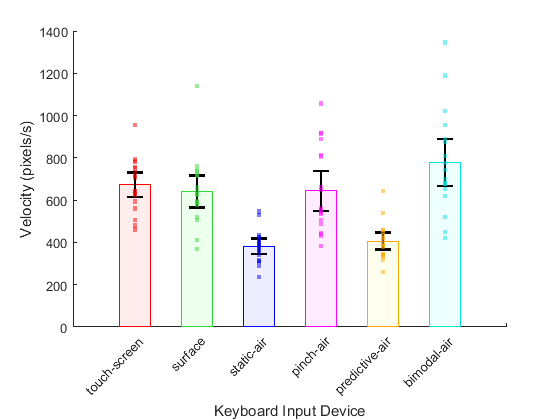
\includegraphics{Figures/fig_velocity_gesture_mean}
	\caption[Mean Word-gesture Velocity]{Mean Word-gesture Velocity for each keyboard with error bars showing 95\% confidence intervals.}
	\label{fig_velocity_gesture_mean}
\end{figure}

The multiple comparisons, seen in Table~\ref{velocity_gesture_multcompare}, revealed significant differences ($p$-values $<$ 0.0001) in Word-gesture Velocity between the Touch Screen Keyboard and the Leap Static-air and Predictive-air keyboards. There were significant differences ($p$-values $<$ 0.001) between the Leap Surface Keyboard and the Static-air and Predictive-air keyboards. There were also significant differences ($p$-values $<$ 0.0001) found between the Leap Bimodal-air and the Static-air and Predictive-air keyboards. Finally, there were significant differences ($p$-values $<$ 0.001) found between the Leap Pinch-air and the Static-air and Predictive Air keyboards.

The Static-air and Predictive-air keyboards were significantly slower than all of the other keyboards for word-gesture velocity. This was expected due to the enhanced precision required when working with a 3rd-dimension in mid-air. It is interesting that these two keyboards also had the highest error rates across all error measures, implying a very high degree of difficulty, even with slower, more precise movements.

\subsection{Hand Velocity}
Participants reached a mean Hand Velocity of 35.7 $cm/s$ ($SD = 6.7$) for the Touch Screen Keyboard, 15.0 $cm/s$ ($SD = 3.9$) for the Leap Surface Keyboard, 6.9 $cm/s$ ($SD = 1.4$) for the Leap Static-air Keyboard, 10.5 $cm/s$ ($SD = 3.2$) for the Leap Pinch-air Keyboard, 7.6 $cm/s$ ($SD = 1.7$) for the Predictive-air Keyboard, and 15.2 $cm/s$ ($SD = 5.1$) for the Leap Bimodal-air Keyboard. Figure~\ref{fig_velocity_hand_mean} shows the mean Hand Velocity for each keyboard interaction style. Using a one-way ANOVA, a significant difference was detected between keyboard means ($F(5, 102) = 121.9826$, $p$-value $<$ 0.0001, $SD_{pooled} = 4.1$), prompting the use of Tukey's HSD with multiple-compare for further analysis.

\begin{figure}[!t]
	\centering
	\includegraphics{Figures/fig_velocity_hand_mean}
	\caption[Mean Hand Velocity]{Mean Hand Velocity for each keyboard with error bars showing 95\% confidence intervals.}
	\label{fig_velocity_hand_mean}
\end{figure}

The multiple comparisons, seen in Table~\ref{velocity_hand_multcompare}, revealed significant differences ($p$-values $<$ 0.0001) in Hand Velocity between the Touch Screen Keyboard and all other keyboards. There were significant differences ($p$-values $<$ 0.05) between the Leap Surface Keyboard and the Static-air, Pinch-air, and Predictive-air keyboards. There were also significant differences ($p$-values $<$ 0.05) found between the Leap Bimodal-air and all other mid-air keyboards.

The hand velocities were all similar to the word-gesture velocities in Section~\ref{results_velocity_gesture}, except for the Touch Screen Keyboard. This result was simply caused by the physical size difference between the interaction planes and the size of the Touch Screen, as mentioned in Chapter~\ref{keyboard_design}.

\section{Time-based Measures}

\subsection{Word-gesture Duration}
Participants reached a mean Word-gesture Duration of 1.65 $s$ ($SD = 0.46$) for the Touch Screen Keyboard, 2.03 $s$ ($SD = 1.17$) for the Leap Surface Keyboard, 4.01 $s$ ($SD = 1.17$) for the Leap Static-air Keyboard, 3.36 $s$ ($SD = 0.76$) for the Leap Pinch-air Keyboard, 3.87 $s$ ($SD = 1.18$) for the Predictive-air Keyboard, and 2.18 $s$ ($SD = 0.36$) for the Leap Bimodal-air Keyboard. Figure~\ref{fig_time_mean} shows the mean Word-gesture Duration for each keyboard interaction style. Using a one-way ANOVA, a significant difference was detected between keyboard means ($F(5, 102) = 28.1205$, $p$-value $<$ 0.0001, $SD_{pooled} = 0.81$), prompting the use of Tukey's HSD with multiple-compare for further analysis.

\begin{figure}[!b]
	\centering
	\includegraphics{Figures/fig_time_mean}
	\caption[Mean Word-gesture Duration]{Mean Word-gesture Duration for each keyboard with error bars showing 95\% confidence intervals.}
	\label{fig_time_mean}
\end{figure}

The multiple comparisons, seen in Table~\ref{time_multcompare}, revealed significant differences ($p$-values $<$ 0.0001) in Word-gesture Duration between the Touch Screen Keyboard and the Leap Static-air, Pinch-air, and Predictive-air keyboards. There were significant differences ($p$-values $<$ 0.001) between the Leap Surface Keyboard and the Static-air, Pinch-air, and Predictive-air keyboards. There were also significant differences ($p$-values $<$ 0.001) found between the Leap Bimodal-air and all of the other mid-air keyboards.

As expected, the Static-air, Pinch-air, and Predictive-air keyboards had significantly longer word-gesture durations than the other keyboards. For the Static-air and Predictive-air, lower velocities and higher decoupling meant that word-gestures take longer to perform, whereas for the Pinch-air Keyboard, the longer distances traveled influenced the longer durations. The Bimodal-air keyboard performed as well as the Touch Screen and Leap Surface keyboards, as expected from its prior trends. 

\subsubsection{Word-gesture duration modified-shortest}
Participants reached a mean Word-gesture Duration of 1.60 $s$ ($SD = 0.40$) for the Touch Screen Keyboard, 2.00 $s$ ($SD = 0.55$) for the Leap Surface Keyboard, 3.75 $s$ ($SD = 0.93$) for the Leap Static-air Keyboard, 3.17 $s$ ($SD = 0.73$) for the Leap Pinch-air Keyboard, 3.56 $s$ ($SD = 0.86$) for the Predictive-air Keyboard, and 2.16 $s$ ($SD = 0.36$) for the Leap Bimodal-air Keyboard. Figure~\ref{fig_time_short_mean} shows the mean Word-gesture Duration with the shortest-transcribed modification for each keyboard interaction style. Using a one-way ANOVA, a significant difference was detected between keyboard means ($F(5, 102) = 32.0355$, $p$-value $<$ 0.0001, $SD_{pooled} = 0.67$), prompting the use of Tukey's HSD with multiple-compare for further analysis.

\begin{figure}[!t]
	\centering
	\includegraphics{Figures/fig_time_short_mean}
	\caption[Mean Word-gesture Duration for Modified-shortest]{Mean Word-gesture Dur using the shortest-transcribed modification for each keyboard with error bars showing 95\% confidence intervals.}
	\label{fig_time_short_mean}
\end{figure}

The multiple comparisons, seen in Table~\ref{time_short_multcompare}, revealed significant differences ($p$-values $<$ 0.0001) in Word-gesture Duration with the shortest-transcribed modification between the Touch Screen Keyboard and the Leap Static-air, Pinch-air, and Predictive-air keyboards. There were significant differences ($p$-values $<$ 0.0001) between the Leap Surface Keyboard and the Leap Static-air, Pinch-air, and Predictive-air keyboards. There were also significant differences ($p$-values $<$ 0.001) found between the Leap Bimodal-air and all of the other mid-air keyboards.

As seen before, the shortest-transcribed modification for word-gesture duration had little effect on the total length of word-gesture durations. This again supported the idea that participants mostly corrected errors as they were being made during transcription.

\subsection{Reaction Time to Errors}
Participants reached a mean Reaction Time to Errors of 0.22 $s$ ($SD = 0.23$) for the Touch Screen Keyboard, 0.40 $s$ ($SD = 0.29$) for the Leap Surface Keyboard, 1.02 $s$ ($SD = 0.43$) for the Leap Static-air Keyboard, 0.59 $s$ ($SD = 0.30$) for the Leap Pinch-air Keyboard, 0.78 $s$ ($SD = 0.40$) for the Predictive-air Keyboard, and 0.29 $s$ ($SD = 0.24$) for the Leap Bimodal-air Keyboard. Figure~\ref{fig_reaction_errors_mean} shows the mean Reaction Time to Errors for each keyboard interaction style. Using a one-way ANOVA, a significant difference was detected between keyboard means ($F(5, 102) = 16.3385$, $p$-value $<$ 0.0001, $SD_{pooled} = 0.32$), prompting the use of Tukey's HSD with multiple-compare for further analysis.

\begin{figure}[!t]
	\centering
	\includegraphics{Figures/fig_reaction_errors_mean}
	\caption[Mean Reaction Time to Errors]{Mean Reaction Time to Errors for each keyboard with error bars showing 95\% confidence intervals.}
	\label{fig_reaction_errors_mean}
\end{figure}

The multiple comparisons, seen in Table~\ref{reaction_errors_multcompare}, revealed significant differences ($p$-values $<$ 0.01) in Reaction Time to Errors between the Touch Screen Keyboard and the Leap Static-air, Pinch-air, and Predictive-air keyboards. There were significant differences ($p$-values $<$ 0.01) between the Leap Surface Keyboard and the Static-air and Predictive-air keyboards. There were also significant differences ($p$-values $<$ 0.001) found between the Leap Bimodal-air and the Static-air and Predictive-air keyboards. Finally, there was a significant difference ($p$-value $=$ 0.0017) found between the Pinch-air and Static-air keyboards.

As expected, keyboards involving the 3rd-dimension had significantly slower response times to errors than keyboards that did not. This implied that these keyboards required a higher degree of focus due to increased decoupling between the motor space and display.

\subsection{Reaction Time to Simulate Touch}
Participants reached a mean Reaction Time to Simulate Touch of 1.24 $s$ ($SD = 0.21$) for the Touch Screen Keyboard, 1.22 $s$ ($SD = 0.40$) for the Leap Surface Keyboard, 2.60 $s$ ($SD = 0.82$) for the Leap Static-air Keyboard, 1.71 $s$ ($SD = 0.37$) for the Leap Pinch-air Keyboard, 2.23 $s$ ($SD = 0.83$) for the Predictive-air Keyboard, and 1.41 $s$ ($SD = 0.23$) for the Leap Bimodal-air Keyboard. Figure~\ref{fig_reaction_touch_mean} shows the mean Reaction Time to Simulate Touch for each keyboard interaction style. Using a one-way ANOVA, a significant difference was detected between keyboard means ($F(5, 102) = 19.6476$, $p$-value $<$ 0.0001, $SD_{pooled} = 0.54$), prompting the use of Tukey's HSD with multiple-compare for further analysis.

\begin{figure}[!t]
	\centering
	\includegraphics{Figures/fig_reaction_touch_mean}
	\caption[Mean Reaction Time to Simulate Touch]{Mean Reaction Time to Simulate Touch for each keyboard with error bars showing 95\% confidence intervals.}
	\label{fig_reaction_touch_mean}
\end{figure}

The multiple comparisons, seen in Table~\ref{reaction_touch_multcompare}, revealed significant differences ($p$-values $<$ 0.0001) in Reaction Time to Simulate Touch between the Touch Screen Keyboard and the Leap Static-air and Predictive-air keyboards. There were significant differences ($p$-values $<$ 0.0001) between the Leap Surface Keyboard and the Static-air and Predictive-air keyboards. There were also significant differences ($p$-values $<$ 0.001) found between the Leap Bimodal-air and the Static-air and Predictive-air keyboards. Finally, a significant difference ($p$-value = 0.0001) was detected between the Pinch-air and Static-air keyboards.

Again, the reaction time to simulate a touch was significantly slower for the Static-air and Predictive-air keyboards due to the introduction of the 3rd-dimension and increased decoupling between the word-gesture motor space and the display.

\subsection{Reaction Time for First Correct Letter}
Participants reached a mean Reaction Time for First Correct Letter of 1.44 $s$ ($SD = 0.33$) for the Touch Screen Keyboard, 1.92 $s$ ($SD = 0.70$) for the Leap Surface Keyboard, 3.68 $s$ ($SD = 1.52$) for the Leap Static-air Keyboard, 2.34 $s$ ($SD = 0.68$) for the Leap Pinch-air Keyboard, 3.40 $s$ ($SD = 1.40$) for the Predictive-air Keyboard, and 1.49 $s$ ($SD = 0.31$) for the Leap Bimodal-air Keyboard. Figure~\ref{fig_reaction_pressed_mean} shows the mean Reaction Time for First Correct Letter for each keyboard interaction style. Using a one-way ANOVA, a significant difference was detected between keyboard means ($F(5, 102) = 18.3416$, $p$-value $<$ 0.0001, $SD_{pooled} = 0.95$), prompting the use of Tukey's HSD with multiple-compare for further analysis.

\begin{figure}[!t]
	\centering
	\includegraphics{Figures/fig_reaction_pressed_mean}
	\caption[Mean Reaction Time for First Correct Letter]{Mean Reaction Time for First Correct Letter for each keyboard with error bars showing 95\% confidence intervals.}
	\label{fig_reaction_pressed_mean}
\end{figure}

The multiple comparisons, seen in Table~\ref{reaction_pressed_multcompare}, revealed significant differences ($p$-values $<$ 0.0001) in Reaction Time for First Correct Letter between the Touch Screen Keyboard and the Leap Static-air and Predictive-air keyboards. There were significant differences ($p$-values $<$ 0.001) between the Leap Surface Keyboard and the Static-air and Predictive-air keyboards. There were also significant differences ($p$-values $<$ 0.0001) found between the Leap Bimodal-air and the Static-air and Predictive-air keyboards. Finally, there were significant differences ($p$-values $<$ 0.05) found between the Leap Pinch-air and the Static-air and Predictive-air keyboards.

The Leap Bimodal-air Keyboard performed at almost exactly the same rate as the Touch Screen Keyboard for entering the first correct character of each word. Although not a significant difference, it should also be noted that the Leap Surface Keyboard performed slightly slower than both the Bimodal-air and Touch Screen keyboards because participants had a tendency to look down at the printed keyboard. If participants had looked at the on-screen keyboard instead, there would have been a major increase in decoupling that would have further slowed the use of the Leap Surface Keyboard.

Again, the reaction time to simulate a touch was significantly slower for the Static-air and Predictive-air keyboards due to the introduction of the 3rd-dimension and increased decoupling between the word-gesture motor space and the display.

\section{Additional Quantitative Measures}

\subsection{Number of Touches Simulated}
Participants reached a mean Number of Touches Simulated of 1.58 simulations ($SD = 0.79$) for the Touch Screen Keyboard, 1.62 simulations ($SD = 0.55$) for the Leap Surface Keyboard, 3.77 simulations ($SD = 2.21$) for the Leap Static-air Keyboard, 2.42 simulations ($SD = 1.05$) for the Leap Pinch-air Keyboard, 3.33 simulations ($SD = 1.62$) for the Predictive-air Keyboard, and 1.67 simulations ($SD = 0.53$) for the Leap Bimodal-air Keyboard. Figure~\ref{fig_num_touches_mean} shows the mean Number of Touches Simulated for each keyboard interaction style. Using a one-way ANOVA, a significant difference was detected between keyboard means ($F(5, 102) = 10.0290$, $p$-value $<$ 0.0001, $SD_{pooled} = 1.28$), prompting the use of Tukey's HSD with multiple-compare for further analysis.

\begin{figure}[!t]
	\centering
	\includegraphics{Figures/fig_num_touches_mean}
	\caption[Mean Number of Touches Simulated]{Mean Number of Touches Simulated for each keyboard with error bars showing 95\% confidence intervals.}
	\label{fig_num_touches_mean}
\end{figure}

The multiple comparisons, seen in Table~\ref{num_touches_multcompare}, revealed significant differences ($p$-values $<$ 0.01) in Number of Touches Simulated between the Touch Screen Keyboard and the Leap Static-air and Predictive-air keyboards. There were significant differences ($p$-values $<$ 0.01) between the Leap Surface Keyboard and the Static-air and Predictive-air keyboards. There were also significant differences ($p$-values $<$ 0.01) found between the Leap Bimodal-air and the Static-air and Predictive-air keyboards. Finally, there was a significant difference ($p$-value = 0.0245) between the Pinch-air keyboard and the Static-air keyboard.

Again, the same trends as before were seen. The Leap Surface and Bimodal-air keyboards performed on par with the Touch Screen Keyboard, the Static-air and Predictive-air keyboards saw significantly more simulated touches, and the Pinch-air keyboard was somewhere in the middle. It was observed that the Static-air keyboard suffered from a ``skimming'' issue. The ``skimming'' issue occurred when participants would only reach far enough to barely simulate a touch on the interaction plane, and then when they would move their hand from one side of the keyboard to the other, the natural arcing motion of the participants' hands would cause them to pull away from the interaction plane as they moved. This issue was assumed to also be a culprit for some of the increased error rates. Figure~\ref{arcing_motion} and Figure~\ref{skimming_problem} both show how the skimming issue worked in detail. % TODO: possibly move skimming problem figure from conclusion to here

\subsection{Number of Practice Words}
Participants reached a mean Number of Practice Words of 5.4 words ($SD = 4.3$) for the Touch Screen Keyboard, 7.7 words ($SD = 3.9$) for the Leap Surface Keyboard, 9.0 words ($SD = 6.7$) for the Leap Static-air Keyboard, 8.1 words ($SD = 5.3$) for the Leap Pinch-air Keyboard, 8.9 words ($SD = 6.8$) for the Predictive-air Keyboard, and 10.2 words ($SD = 3.9$) for the Leap Bimodal-air Keyboard. Figure~\ref{fig_num_practice_mean} shows the mean Number of Practice Words for each keyboard interaction style. Using a one-way ANOVA, no significant differences were detected between keyboard means ($F(5, 102) = 1.6828$, $p$-value = 0.1454, $SD_{pooled} = 5.3$), therefore no additional analysis was made. Typically, as observed by the researcher, there were two categories of participants when it came to performing practice words. The first category contained participants who would perform a full set of 15 words for each keyboard. Rarely, these participants felt the need to perform more than one practice set's worth of words. The second category contained participants who progressively performed less practice words for each consecutive keyboard; this is a primary example of why a Replicated Latin Squares design for counterbalancing was used.

\begin{figure}[!t]
	\centering
	\includegraphics{Figures/fig_num_practice_mean}
	\caption[Mean Number of Practice Words]{Mean Number of Practice Words for each keyboard with error bars showing 95\% confidence intervals.}
	\label{fig_num_practice_mean}
\end{figure}

\section{Qualitative Measures}
\subsection{Level of Discomfort}
%means = -1.7222   -1.5556   -0.2778   -0.7778   -0.3889   -1.2778
%stds = 0.7519    0.6157    1.0741    0.9428    1.3346    0.7519
Keyboards reached a median Level of Discomfort of ``Strongly Disagree'' for the Touch Screen Keyboard, ``Strongly Disagree'' for the Leap Surface Keyboard, ``Neutral'' for the Leap Static-air Keyboard, ``Disagree'' for the Leap Pinch-air Keyboard, between ``Disagree'' and ``Neutral'' for the Predictive-air Keyboard, and ``Disagree'' for the Leap Bimodal-air Keyboard. Figure~\ref{fig_discomfort_boxplot} shows the median Level of Discomfort for each keyboard interaction style rated by the participants. Using a one-way ANOVA, a significant difference was detected between keyboard means for Level of Discomfort ($F(5, 102) = 7.5000$, $p$-value $<$ 0.0001, $SD_{pooled} = 0.94$), prompting the use of Tukey's HSD with multiple-compare for further analysis.

\begin{figure}[!t]
	\centering
	\includegraphics{Figures/fig_discomfort_boxplot}
	\caption[Level of Discomfort Boxplot]{Median Level of Discomfort for each keyboard showing the 25th and 75th percentiles.}
	\label{fig_discomfort_boxplot}
\end{figure}

The multiple comparisons, seen in Table~\ref{discomfort_multcompare}, revealed significant differences ($p$-values $<$ 0.05) in Level of Discomfort between the Touch Screen Keyboard and the Leap Static-air, Pinch-air, and Predictive-air keyboards. There were significant differences ($p$-values $<$ 0.01) between the Leap Surface Keyboard and the Static-air and Predictive-air keyboards. There was also a significant difference ($p$-value $=$ 0.0232) found between the Leap Bimodal-air and the Static-air keyboards with.

The level of discomfort experienced by participants, not surprisingly, was very similar to the trend seen in most other dependent measures. Discomfort was experienced more for the mid-air keyboards, and more extremely by the keyboards that utilized the extra degree of freedom available in the 3rd-dimension.

\subsection{Level of Fatigue}
%means = -1.6111   -1.2778    0.7778   -0.0556   -0.1111   -0.6111
%stds = 0.6978    1.0741    1.1660    1.2590    1.0786    1.3346
Keyboards reached a median Level of Fatigue of ``Strongly Disagree'' for the Touch Screen Keyboard, ``Strongly Disagree'' for the Leap Surface Keyboard, ``Agree'' for the Leap Static-air Keyboard, between ``Neutral'' and ``Agree'' for the Leap Pinch-air Keyboard, ``Neutral'' for the Predictive-air Keyboard, and ``Disagree'' for the Leap Bimodal-air Keyboard. Figure~\ref{fig_fatigue_boxplot} shows the median Level of Fatigue for each keyboard interaction style rated by the participants. Using a one-way ANOVA, a significant difference was detected between keyboard means for Level of Discomfort ($F(5, 102) = 10.9910$, $p$-value $<$ 0.0001, $SD_{pooled} = 1.12$), prompting the use of Tukey's HSD with multiple-compare for further analysis.

\begin{figure}[!t]
	\centering
	\includegraphics{Figures/fig_fatigue_boxplot}
	\caption[Level of Fatigue Boxplot]{Median Level of Fatigue for each keyboard showing the 25th and 75th percentiles.}
	\label{fig_fatigue_boxplot}
\end{figure}

The multiple comparisons, seen in Table~\ref{fatigue_multcompare}, revealed significant differences ($p$-values $<$ 0.01) in Level of Fatigue between the Touch Screen Keyboard and the Leap Static-air, Pinch-air, and Predictive-air keyboards. There were significant differences ($p$-values $<$ 0.05) between the Leap Surface Keyboard and the Static-air, Pinch-air, and Predictive-air keyboards. There was also a significant difference ($p$-value $=$ 0.0043) found between the Leap Bimodal-air and the Static-air keyboards. As expected, the fatigue levels experienced for mid-air keyboards were typically higher than those that were not mid-air.

\subsection{Level of Difficulty}
%means = -1.7222   -1.4444   -0.2222   -0.6667   -0.6667   -1.2778
%stds = 0.5745    0.7048    1.1144    1.1882    1.2834    0.8264
Keyboards reached a median Level of Difficulty of ``Strongly Disagree'' for the Touch Screen Keyboard, ``Strongly Disagree'' for the Leap Surface Keyboard, between ``Disagree'' and ``Neutral'' for the Leap Static-air Keyboard, ``Disagree'' for the Leap Pinch-air Keyboard, ``Disagree'' for the Predictive-air Keyboard, and ``Disagree'' for the Leap Bimodal-air Keyboard. Figure~\ref{fig_difficulty_boxplot} shows the median Level of Difficulty for each keyboard interaction style rated by the participants. Using a one-way ANOVA, a significant difference was detected between keyboard means for Level of Discomfort ($F(5, 102) = 6.0351$, $p$-value $<$ 0.0001, $SD_{pooled} = 0.98$), prompting the use of Tukey's HSD with multiple-compare for further analysis.

\begin{figure}[!t]
	\centering
	\includegraphics{Figures/fig_difficulty_boxplot}
	\caption[Level of Difficulty Boxplot]{Median Level of Difficulty for each keyboard showing the 25th and 75th percentiles.}
	\label{fig_difficulty_boxplot}
\end{figure}

The multiple comparisons, seen in Table~\ref{difficulty_multcompare}, revealed significant differences ($p$-values $<$ 0.05) in Level of Difficulty between the Touch Screen Keyboard and the Leap Static-air, Pinch-air, and Predictive-air keyboards. There was significant difference ($p$-values $=$ 0.0042) between the Leap Surface and the Static-air keyboards. There was also a significant difference ($p$-value $=$ 0.0209) found between the Leap Bimodal-air and the Static-air keyboards. As anticipated, the mid-air keyboards had a higher level of difficulty and were harder to use or understand than the non-mid-air keyboards.

\subsection{Preference Ranking}
Participants reached a mean Preference Ranking of 1.89 ($SD = 1.18$) for the Touch Screen Keyboard, 2.22 ($SD = 1.22$) for the Leap Surface Keyboard, 5.33 ($SD = 0.84$) for the Leap Static-air Keyboard, 4.22 ($SD = 1.06$) for the Leap Pinch-air Keyboard, 4.50 ($SD = 1.42$) for the Predictive-air Keyboard, and 2.83 ($SD = 1.29$) for the Leap Bimodal-air Keyboard. Figure~\ref{fig_ranking_mean} shows the mean Preference Ranking for each keyboard interaction style. Using Friedman's rank-test, ANOVA, a significant difference was detected between keyboard means, $\chi^{2}(5, 85) = 49.1429$, $p$-value $<$ 0.0001, $SD_{pooled} = 1.87$), prompting the use of Tukey's HSD with multiple-compare for further analysis.

\begin{figure}[!t]
	\centering
	\includegraphics{Figures/fig_ranking_mean}
	\caption[Mean Preference Rankings]{Mean Preference Rankings for each keyboard with error bars showing 95\% confidence intervals.}
	\label{fig_ranking_mean}
\end{figure}

The multiple comparisons, seen in Table~\ref{ranking_multcompare}, revealed significant differences ($p$-values $<$ 0.01) in Preference Ranking between the Touch Screen Keyboard and the Leap Static-air, Pinch-air, and Predictive-air keyboards. There were significant differences ($p$-values $<$ 0.05) between the Leap Surface Keyboard and the Static-air, Pinch-air, and Predictive-air keyboards. There was also a significant difference ($p$-value $=$ 0.0009) found between the Leap Bimodal-air and the Static-air keyboards.

The preference ranking of all of the keyboards very strongly reflected the trends seen in most of the other dependent measures. The Touch Screen Keyboard was the most preferred, as expected, followed by the Leap Surface in a close second. The Leap Bimodal-air was the most preferred mid-air keyboard, whereas the Static-air Keyboard was the least preferred.
	
	% Appendices (optional)
	% TODO: make the thesisAppendixPage automagic if the \begin{appendices} exists
	\thesisAppendixPage 
	\begin{appendices}
		\chapter{Word-Gesturing Implementation}

		\chapter{Results Tables and Boxplots}
The statistical methods used consisted of One-Way ANOVAs for each set of the dependent measures, followed by using Tukey's Honest Significant Difference (HSD) for multiple-compare for the post-hoc analysis. The ranking system from the exit survey used the Friedman's test for analysis in conjunction with Tukey's HSD for a post-hoc analysis.

\clearpage
\section{Text-Entry Rate}
\begin{figure}[h]
	\centering
	\includegraphics{fig_textentry_boxplot}
	\caption[Text-Entry Rate Boxplot]{Median Text-Entry Rates for each keyboard showing the 25th and 75th percentiles.}
	\label{fig_textentry_boxplot}
\end{figure}

\begin{table}[h]
	\centering
	\caption[Text-Entry Rate Multiple Comparison]{\centering Tukey's Honest Significant Difference with multiple comparison for Text-Entry Rate.}
	\label{textentry_multcompare}
	\resizebox{\textwidth}{!}{\begin{tabular}{ l l r r r r }
		\hline
		\multirow{2}{*}{Group 1} & \multirow{2}{*}{Group 2} & Confidience Interval & Mean Difference & Confidience Interval & \multirow{2}{*}{$p$-value} \\
		{} & {} & Lower End & $\mu_1 - \mu_2$ & Upper End & {} \\
		\hline
		touchscreen & surface & -0.0837 & 2.3522 & 4.7882 & 0.0648 \\
		touchscreen & static-air & 8.4479 & 10.8839 & 13.3198 & 0.0000 \\
		touchscreen & pinch-air & 5.6920 & 8.1280 & 10.5639 & 0.0000 \\
		touchscreen & predictive-air & 7.4227 & 9.8587 & 12.2946 & 0.0000 \\
		touchscreen & bimodal-air & 1.2832 & 3.7192 & 6.1551 & 0.0003 \\
		surface & static-air & 6.0957 & 8.5316 & 10.9676 & 0.0000 \\
		surface & pinch-air & 3.3398 & 5.7757 & 8.2117 & 0.0000 \\
		surface & predictive-air & 5.0705 & 7.5064 & 9.9424 & 0.0000 \\
		surface & bimodal-air & -1.0690 & 1.3669 & 3.8029 & 0.5809 \\
		static-air & pinch-air & -5.1919 & -2.7559 & -0.3199 & 0.0170 \\
		static-air & predictive-air & -3.4612 & -1.0252 & 1.4108 & 0.8249 \\
		static-air & bimodal-air & -9.6007 & -7.1647 & -4.7287 & 0.0000 \\
		pinch-air & predictive-air & -0.7053 & 1.7307 & 4.1667 & 0.3146 \\
		pinch-air & bimodal-air & -6.8448 & -4.4088 & -1.9728 & 0.0000 \\
		predictive-air & bimodal-air & -8.5755 & -6.1395 & -3.7035 & 0.0000 \\
		\hline
	\end{tabular}}
\end{table}

\clearpage
\subsection{Text-Entry Rate Modified-Shortest}
\begin{figure}[h]
	\centering
	\includegraphics{fig_textentry_short_boxplot}
	\caption[Text-Entry Rates Boxplot for Modified-Shortest]{Median Text-Entry Rates using the shortest-transcribed modification for each keyboard showing the 25th and 75th percentiles.}
	\label{fig_textentry_short_boxplot}
\end{figure}

\begin{table}[h]
\centering
\caption[Text-Entry Rate Multiple Comparison Modified-Shortest]{\centering Tukey's Honest Significant Difference with multiple comparison for Text-Entry Rate modified with shortest-transcribed.}
\label{textentry_short_multcompare}
\resizebox{\textwidth}{!}{\begin{tabular}{ l l r r r r }
\hline
\multirow{2}{*}{Group 1} & \multirow{2}{*}{Group 2} & Confidience Interval & Mean Difference & Confidience Interval & \multirow{2}{*}{$p$-value} \\
{} & {} & Lower End & $\mu_1 - \mu_2$ & Upper End & {} \\
\hline
touchscreen & surface & -0.0162 & 2.4063 & 4.8288 & 0.0526 \\
touchscreen & static-air & 8.4069 & 10.8295 & 13.2520 & 0.0000 \\
touchscreen & pinch-air & 5.6271 & 8.0496 & 10.4722 & 0.0000 \\
touchscreen & predictive-air & 7.3096 & 9.7321 & 12.1546 & 0.0000 \\
touchscreen & bimodal-air & 1.3652 & 3.7877 & 6.2103 & 0.0002 \\
surface & static-air & 6.0006 & 8.4232 & 10.8457 & 0.0000 \\
surface & pinch-air & 3.2208 & 5.6433 & 8.0659 & 0.0000 \\
surface & predictive-air & 4.9033 & 7.3258 & 9.7483 & 0.0000 \\
surface & bimodal-air & -1.0411 & 1.3814 & 3.8040 & 0.5636 \\
static-air & pinch-air & -5.2024 & -2.7798 & -0.3573 & 0.0148 \\
static-air & predictive-air & -3.5199 & -1.0974 & 1.3251 & 0.7757 \\
static-air & bimodal-air & -9.4643 & -7.0417 & -4.6192 & 0.0000 \\
pinch-air & predictive-air & -0.7401 & 1.6825 & 4.1050 & 0.3399 \\
pinch-air & bimodal-air & -6.6844 & -4.2619 & -1.8394 & 0.0000 \\
predictive-air & bimodal-air & -8.3669 & -5.9443 & -3.5218 & 0.0000 \\
\hline
\end{tabular}}
\end{table}

\clearpage
\section{Error Rates}
\subsection{Minimum Word Distance}
\begin{figure}[h]
	\centering
	\includegraphics{fig_MWD_boxplot}
	\caption[Minimum Word Distance Boxplot]{Median Minimum Word Distance for each keyboard showing the 25th and 75th percentiles.}
	\label{fig_MWD_boxplot}
\end{figure}

\begin{table}[h]
\centering
\caption[MWD Multiple Comparison]{\centering Tukey's Honest Significant Difference with multiple comparison for Minimum Word Distance.}
\label{MWD_multcompare}
\resizebox{\textwidth}{!}{\begin{tabular}{ l l r r r r }
\hline
\multirow{2}{*}{Group 1} & \multirow{2}{*}{Group 2} & Confidience Interval & Mean Difference & Confidience Interval & \multirow{2}{*}{$p$-value} \\
{} & {} & Lower End & $\mu_1 - \mu_2$ & Upper End & {} \\
\hline
touchscreen & surface & -23.8140 & -5.9259 & 11.9622 & 0.9287 \\
touchscreen & static-air & -61.5918 & -43.7037 & -25.8156 & 0.0000 \\
touchscreen & pinch-air & -39.3696 & -21.4815 & -3.5934 & 0.0091 \\
touchscreen & predictive-air & -53.8140 & -35.9259 & -18.0378 & 0.0000 \\
touchscreen & bimodal-air & -25.2955 & -7.4074 & 10.4807 & 0.8346 \\
surface & static-air & -55.6659 & -37.7778 & -19.8897 & 0.0000 \\
surface & pinch-air & -33.4437 & -15.5556 & 2.3326 & 0.1263 \\
surface & predictive-air & -47.8881 & -30.0000 & -12.1119 & 0.0001 \\
surface & bimodal-air & -19.3696 & -1.4815 & 16.4066 & 0.9999 \\
static-air & pinch-air & 4.3341 & 22.2222 & 40.1103 & 0.0062 \\
static-air & predictive-air & -10.1103 & 7.7778 & 25.6659 & 0.8043 \\
static-air & bimodal-air & 18.4082 & 36.2963 & 54.1844 & 0.0000 \\
pinch-air & predictive-air & -32.3326 & -14.4444 & 3.4437 & 0.1859 \\
pinch-air & bimodal-air & -3.8140 & 14.0741 & 31.9622 & 0.2096 \\
predictive-air & bimodal-air & 10.6304 & 28.5185 & 46.4066 & 0.0002 \\
\hline
\end{tabular}}
\end{table}

\clearpage
\subsubsection{MWD Modified-Shortest}
\begin{figure}[h]
	\centering
	\includegraphics{fig_MWD_short_boxplot}
	\caption[Minimum Word Distance Boxplot for Modified-Shortest]{Median Minimum Word Distance using the shortest-transcribed modification for each keyboard showing the 25th and 75th percentiles.}
	\label{fig_MWD_short_boxplot}
\end{figure}

\begin{table}[h]
\centering
\caption[MWD Multiple Comparison Modified-Shortest]{\centering Tukey's Honest Significant Difference with multiple comparison for Minimum Word Distance using shortest-transcribed modification.}
\label{MWD_short_multcompare}
\resizebox{\textwidth}{!}{\begin{tabular}{ l l r r r r }
\hline
\multirow{2}{*}{Group 1} & \multirow{2}{*}{Group 2} & Confidience Interval & Mean Difference & Confidience Interval & \multirow{2}{*}{$p$-value} \\
{} & {} & Lower End & $\mu_1 - \mu_2$ & Upper End & {} \\
\hline
touchscreen & surface & -13.0458 & 0.0000 & 13.0458 & 1.0000 \\
touchscreen & static-air & -32.3051 & -19.2593 & -6.2135 & 0.0006 \\
touchscreen & pinch-air & -26.7495 & -13.7037 & -0.6579 & 0.0336 \\
touchscreen & predictive-air & -32.6754 & -19.6296 & -6.5838 & 0.0004 \\
touchscreen & bimodal-air & -16.7495 & -3.7037 & 9.3421 & 0.9623 \\
surface & static-air & -32.3051 & -19.2593 & -6.2135 & 0.0006 \\
surface & pinch-air & -26.7495 & -13.7037 & -0.6579 & 0.0336 \\
surface & predictive-air & -32.6754 & -19.6296 & -6.5838 & 0.0004 \\
surface & bimodal-air & -16.7495 & -3.7037 & 9.3421 & 0.9623 \\
static-air & pinch-air & -7.4902 & 5.5556 & 18.6013 & 0.8177 \\
static-air & predictive-air & -13.4162 & -0.3704 & 12.6754 & 1.0000 \\
static-air & bimodal-air & 2.5098 & 15.5556 & 28.6013 & 0.0099 \\
pinch-air & predictive-air & -18.9717 & -5.9259 & 7.1199 & 0.7737 \\
pinch-air & bimodal-air & -3.0458 & 10.0000 & 23.0458 & 0.2349 \\
predictive-air & bimodal-air & 2.8801 & 15.9259 & 28.9717 & 0.0076 \\
\hline
\end{tabular}}
\end{table}

\clearpage
\subsection{Keystrokes Per Character}
\begin{figure}[h]
	\centering
	\includegraphics{fig_KSPC_boxplot}
	\caption[Keystrokes Per Character Boxplot]{Median Keystrokes Per Character for each keyboard showing the 25th and 75th percentiles.}
	\label{fig_KSPC_boxplot}
\end{figure}

\begin{table}[h]
\centering
\caption[KSPC Multiple Comparison]{\centering Tukey's Honest Significant Difference with multiple comparison for Keystrokes Per Character.}
\label{KSPC_multcompare}
\resizebox{\textwidth}{!}{\begin{tabular}{ l l r r r r }
\hline
\multirow{2}{*}{Group 1} & \multirow{2}{*}{Group 2} & Confidience Interval & Mean Difference & Confidience Interval & \multirow{2}{*}{$p$-value} \\
{} & {} & Lower End & $\mu_1 - \mu_2$ & Upper End & {} \\
\hline
touchscreen & surface & -0.7298 & -0.2597 & 0.2103 & 0.5972 \\
touchscreen & static-air & -1.3559 & -0.8859 & -0.4158 & 0.0000 \\
touchscreen & pinch-air & -0.8998 & -0.4298 & 0.0403 & 0.0935 \\
touchscreen & predictive-air & -1.2113 & -0.7412 & -0.2712 & 0.0002 \\
touchscreen & bimodal-air & -0.5324 & -0.0623 & 0.4077 & 0.9989 \\
surface & static-air & -1.0962 & -0.6262 & -0.1561 & 0.0026 \\
surface & pinch-air & -0.6401 & -0.1701 & 0.3000 & 0.8993 \\
surface & predictive-air & -0.9515 & -0.4815 & -0.0114 & 0.0414 \\
surface & bimodal-air & -0.2726 & 0.1974 & 0.6675 & 0.8262 \\
static-air & pinch-air & -0.0140 & 0.4561 & 0.9262 & 0.0626 \\
static-air & predictive-air & -0.3254 & 0.1447 & 0.6147 & 0.9471 \\
static-air & bimodal-air & 0.3535 & 0.8236 & 1.2936 & 0.0000 \\
pinch-air & predictive-air & -0.7815 & -0.3114 & 0.1586 & 0.3935 \\
pinch-air & bimodal-air & -0.1026 & 0.3675 & 0.8375 & 0.2157 \\
predictive-air & bimodal-air & 0.2089 & 0.6789 & 1.1490 & 0.0008 \\
\hline
\end{tabular}}
\end{table}

\clearpage
\subsubsection{KSPC Modified-Shortest}
\begin{figure}[h]
	\centering
	\includegraphics{fig_KSPC_short_boxplot}
	\caption[Keystrokes Per Character Boxplot for Modified-Shortest]{Median Keystrokes Per Character using the shortest-transcribed modification for each keyboard showing the 25th and 75th percentiles.}
	\label{fig_KSPC_short_boxplot}
\end{figure}

\begin{table}[h]
\centering
\caption[KSPC Multiple Comparison Modified-Shortest]{\centering Tukey's Honest Significant Difference with multiple comparison for Keystrokes Per Character using shortest-transcribed modification.}
\label{KSPC_short_multcompare}
\resizebox{\textwidth}{!}{\begin{tabular}{ l l r r r r }
\hline
\multirow{2}{*}{Group 1} & \multirow{2}{*}{Group 2} & Confidience Interval & Mean Difference & Confidience Interval & \multirow{2}{*}{$p$-value} \\
{} & {} & Lower End & $\mu_1 - \mu_2$ & Upper End & {} \\
\hline
touchscreen & surface & -0.5181 & -0.2055 & 0.1070 & 0.4020 \\
touchscreen & static-air & -0.9366 & -0.6240 & -0.3115 & 0.0000 \\
touchscreen & pinch-air & -0.5532 & -0.2407 & 0.0719 & 0.2304 \\
touchscreen & predictive-air & -0.8488 & -0.5363 & -0.2237 & 0.0000 \\
touchscreen & bimodal-air & -0.3346 & -0.0220 & 0.2906 & 0.9999 \\
surface & static-air & -0.7310 & -0.4185 & -0.1059 & 0.0024 \\
surface & pinch-air & -0.3477 & -0.0351 & 0.2774 & 0.9995 \\
surface & predictive-air & -0.6433 & -0.3307 & -0.0182 & 0.0316 \\
surface & bimodal-air & -0.1290 & 0.1835 & 0.4961 & 0.5313 \\
static-air & pinch-air & 0.0708 & 0.3833 & 0.6959 & 0.0072 \\
static-air & predictive-air & -0.2248 & 0.0877 & 0.4003 & 0.9641 \\
static-air & bimodal-air & 0.2895 & 0.6020 & 0.9146 & 0.0000 \\
pinch-air & predictive-air & -0.6082 & -0.2956 & 0.0169 & 0.0748 \\
pinch-air & bimodal-air & -0.0939 & 0.2187 & 0.5312 & 0.3316 \\
predictive-air & bimodal-air & 0.2017 & 0.5143 & 0.8269 & 0.0001 \\
\hline
\end{tabular}}
\end{table}

\clearpage
\subsection{Minimum String Distance}
\subsubsection{MSD Modified-Shortest}
\begin{figure}[h]
	\centering
	\includegraphics{fig_MSD_short_boxplot}
	\caption[Minimum String Distance Boxplot for Modified-Shortest]{Median Minimum String Distance using the shortest-transcribed modification for each keyboard showing the 25th and 75th percentiles.}
	\label{fig_MSD_short_boxplot}
\end{figure}

\begin{table}[h]
\centering
\caption[MSD Multiple Comparison Modified-Shortest]{\centering Tukey's Honest Significant Difference with multiple comparison for Minimum String Distance using shortest-transcribed modification.}
\label{MSD_short_multcompare}
\resizebox{\textwidth}{!}{\begin{tabular}{ l l r r r r }
\hline
\multirow{2}{*}{Group 1} & \multirow{2}{*}{Group 2} & Confidience Interval & Mean Difference & Confidience Interval & \multirow{2}{*}{$p$-value} \\
{} & {} & Lower End & $\mu_1 - \mu_2$ & Upper End & {} \\
\hline
touchscreen & surface & -3.7747 & -0.6145 & 2.5457 & 0.9931 \\
touchscreen & static-air & -7.9973 & -4.8372 & -1.6770 & 0.0003 \\
touchscreen & pinch-air & -6.7038 & -3.5437 & -0.3835 & 0.0186 \\
touchscreen & predictive-air & -6.9953 & -3.8351 & -0.6749 & 0.0081 \\
touchscreen & bimodal-air & -4.0980 & -0.9378 & 2.2223 & 0.9546 \\
surface & static-air & -7.3828 & -4.2227 & -1.0625 & 0.0025 \\
surface & pinch-air & -6.0893 & -2.9292 & 0.2310 & 0.0856 \\
surface & predictive-air & -6.3808 & -3.2206 & -0.0604 & 0.0431 \\
surface & bimodal-air & -3.4835 & -0.3233 & 2.8368 & 0.9997 \\
static-air & pinch-air & -1.8667 & 1.2935 & 4.4537 & 0.8412 \\
static-air & predictive-air & -2.1581 & 1.0021 & 4.1622 & 0.9403 \\
static-air & bimodal-air & 0.7392 & 3.8993 & 7.0595 & 0.0067 \\
pinch-air & predictive-air & -3.4516 & -0.2914 & 2.8687 & 0.9998 \\
pinch-air & bimodal-air & -0.5543 & 2.6058 & 5.7660 & 0.1677 \\
predictive-air & bimodal-air & -0.2629 & 2.8973 & 6.0574 & 0.0919 \\
\hline
\end{tabular}}
\end{table}

\clearpage
\subsection{Total Error Rate}
\begin{figure}[h]
	\centering
	\includegraphics{fig_totER_boxplot}
	\caption[Total Error Rate Boxplot]{Median Total Error Rate for each keyboard showing the 25th and 75th percentiles.}
	\label{fig_totER_boxplot}
\end{figure}

\begin{table}[h]
\centering
\caption[Total Error Rate Multiple Comparison]{\centering Tukey's Honest Significant Difference with multiple comparison for Total Error Rate.}
\label{totER_multcompare}
\resizebox{\textwidth}{!}{\begin{tabular}{ l l r r r r }
\hline
\multirow{2}{*}{Group 1} & \multirow{2}{*}{Group 2} & Confidience Interval & Mean Difference & Confidience Interval & \multirow{2}{*}{$p$-value} \\
{} & {} & Lower End & $\mu_1 - \mu_2$ & Upper End & {} \\
\hline
touchscreen & surface & -12.9197 & -4.3716 & 4.1766 & 0.6743 \\
touchscreen & static-air & -27.2196 & -18.6714 & -10.1233 & 0.0000 \\
touchscreen & pinch-air & -17.6640 & -9.1158 & -0.5677 & 0.0295 \\
touchscreen & predictive-air & -23.6696 & -15.1214 & -6.5733 & 0.0000 \\
touchscreen & bimodal-air & -10.4357 & -1.8875 & 6.6606 & 0.9875 \\
surface & static-air & -22.8480 & -14.2999 & -5.7517 & 0.0001 \\
surface & pinch-air & -13.2924 & -4.7443 & 3.8039 & 0.5926 \\
surface & predictive-air & -19.2980 & -10.7498 & -2.2017 & 0.0054 \\
surface & bimodal-air & -6.0641 & 2.4840 & 11.0322 & 0.9584 \\
static-air & pinch-air & 1.0075 & 9.5556 & 18.1038 & 0.0191 \\
static-air & predictive-air & -4.9981 & 3.5500 & 12.0982 & 0.8329 \\
static-air & bimodal-air & 8.2358 & 16.7839 & 25.3321 & 0.0000 \\
pinch-air & predictive-air & -14.5537 & -6.0056 & 2.5425 & 0.3270 \\
pinch-air & bimodal-air & -1.3198 & 7.2283 & 15.7764 & 0.1473 \\
predictive-air & bimodal-air & 4.6858 & 13.2339 & 21.7820 & 0.0003 \\
\hline
\end{tabular}}
\end{table}

\clearpage
\subsubsection{Total Error Rate Modified-Shortest}
\begin{figure}[h]
	\centering
	\includegraphics{fig_totER_short_boxplot}
	\caption[Total Error Rate Boxplot for Modified-Shortest]{Median Total Error Rate using the shortest-transcribed modification for each keyboard showing the 25th and 75th percentiles.}
	\label{fig_totER_short_boxplot}
\end{figure}

\begin{table}[h]
\centering
\caption[Total Error Rate Multiple Comparison Modified-Shortest]{\centering Tukey's Honest Significant Difference with multiple comparison for Total Error Rate using shortest-transcribed modification.}
\label{totER_short_multcompare}
\resizebox{\textwidth}{!}{\begin{tabular}{ l l r r r r }
\hline
\multirow{2}{*}{Group 1} & \multirow{2}{*}{Group 2} & Confidience Interval & Mean Difference & Confidience Interval & \multirow{2}{*}{$p$-value} \\
{} & {} & Lower End & $\mu_1 - \mu_2$ & Upper End & {} \\
\hline
touchscreen & surface & -12.6316 & -4.3367 & 3.9581 & 0.6532 \\
touchscreen & static-air & -26.7322 & -18.4374 & -10.1426 & 0.0000 \\
touchscreen & pinch-air & -16.8635 & -8.5686 & -0.2738 & 0.0386 \\
touchscreen & predictive-air & -22.7732 & -14.4783 & -6.1835 & 0.0000 \\
touchscreen & bimodal-air & -10.1405 & -1.8456 & 6.4492 & 0.9871 \\
surface & static-air & -22.3955 & -14.1007 & -5.8058 & 0.0000 \\
surface & pinch-air & -12.5268 & -4.2319 & 4.0629 & 0.6765 \\
surface & predictive-air & -18.4364 & -10.1416 & -1.8468 & 0.0075 \\
surface & bimodal-air & -5.8037 & 2.4911 & 10.7859 & 0.9523 \\
static-air & pinch-air & 1.5739 & 9.8688 & 18.1636 & 0.0101 \\
static-air & predictive-air & -4.3358 & 3.9591 & 12.2539 & 0.7351 \\
static-air & bimodal-air & 8.2969 & 16.5918 & 24.8866 & 0.0000 \\
pinch-air & predictive-air & -14.2045 & -5.9097 & 2.3851 & 0.3116 \\
pinch-air & bimodal-air & -1.5718 & 6.7230 & 15.0178 & 0.1826 \\
predictive-air & bimodal-air & 4.3379 & 12.6327 & 20.9275 & 0.0003 \\
\hline
\end{tabular}}
\end{table}

\clearpage
\section{Correctness}
\subsection{Fr\'echet Distance}
\begin{figure}[h]
	\centering
	\includegraphics{fig_frechet_boxplot}
	\caption[Fr\'echet Distance Boxplot]{Median Fr\'echet Distance for each keyboard showing the 25th and 75th percentiles.}
	\label{fig_frechet_boxplot}
\end{figure}

\begin{table}[h]
\centering
\caption[Fr\'echet Distance Multiple Comparison]{\centering Tukey's Honest Significant Difference with multiple comparison for Fr\'echet Distance.}
\label{frechet_multcompare}
\resizebox{\textwidth}{!}{\begin{tabular}{ l l r r r r }
\hline
\multirow{2}{*}{Group 1} & \multirow{2}{*}{Group 2} & Confidience Interval & Mean Difference & Confidience Interval & \multirow{2}{*}{$p$-value} \\
{} & {} & Lower End & $\mu_1 - \mu_2$ & Upper End & {} \\
\hline
touchscreen & surface & -78.8540 & -11.6328 & 55.5884 & 0.9960 \\
touchscreen & static-air & -200.3012 & -133.0800 & -65.8588 & 0.0000 \\
touchscreen & pinch-air & -337.2356 & -270.0144 & -202.7931 & 0.0000 \\
touchscreen & predictive-air & -186.6273 & -119.4061 & -52.1849 & 0.0000 \\
touchscreen & bimodal-air & -232.5464 & -165.3252 & -98.1040 & 0.0000 \\
surface & static-air & -188.6684 & -121.4472 & -54.2260 & 0.0000 \\
surface & pinch-air & -325.6027 & -258.3815 & -191.1603 & 0.0000 \\
surface & predictive-air & -174.9945 & -107.7733 & -40.5521 & 0.0001 \\
surface & bimodal-air & -220.9136 & -153.6924 & -86.4712 & 0.0000 \\
static-air & pinch-air & -204.1555 & -136.9343 & -69.7131 & 0.0000 \\
static-air & predictive-air & -53.5473 & 13.6739 & 80.8951 & 0.9914 \\
static-air & bimodal-air & -99.4664 & -32.2452 & 34.9760 & 0.7309 \\
pinch-air & predictive-air & 83.3870 & 150.6083 & 217.8295 & 0.0000 \\
pinch-air & bimodal-air & 37.4679 & 104.6891 & 171.9103 & 0.0002 \\
predictive-air & bimodal-air & -113.1403 & -45.9191 & 21.3021 & 0.3586 \\
\hline
\end{tabular}}
\end{table}

\clearpage
\subsubsection{Fr\'echet Distance Modified-Shortest}
\begin{figure}[h]
	\centering
	\includegraphics{fig_frechet_short_boxplot}
	\caption[Fr\'echet Distance Boxplot for Modified-Shortest]{Median Fr\'echet Distance using the shortest-transcribed modification for each keyboard showing the 25th and 75th percentiles.}
	\label{fig_frechet_short_boxplot}
\end{figure}

\begin{table}[h]
\centering
\caption[Fr\'echet Distance Multiple Comparison Modified-Shortest]{\centering Tukey's Honest Significant Difference with multiple comparison for Fr\'echet Distance using shortest-transcribed modification.}
\label{frechet_short_multcompare}
\resizebox{\textwidth}{!}{\begin{tabular}{ l l r r r r }
\hline
\multirow{2}{*}{Group 1} & \multirow{2}{*}{Group 2} & Confidience Interval & Mean Difference & Confidience Interval & \multirow{2}{*}{$p$-value} \\
{} & {} & Lower End & $\mu_1 - \mu_2$ & Upper End & {} \\
\hline
touchscreen & surface & -55.6656 & -9.9934 & 35.6788 & 0.9881 \\
touchscreen & static-air & -131.1279 & -85.4556 & -39.7834 & 0.0000 \\
touchscreen & pinch-air & -283.8592 & -238.1870 & -192.5147 & 0.0000 \\
touchscreen & predictive-air & -106.2951 & -60.6229 & -14.9506 & 0.0027 \\
touchscreen & bimodal-air & -193.0612 & -147.3890 & -101.7167 & 0.0000 \\
surface & static-air & -121.1345 & -75.4622 & -29.7900 & 0.0001 \\
surface & pinch-air & -273.8658 & -228.1936 & -182.5213 & 0.0000 \\
surface & predictive-air & -96.3017 & -50.6295 & -4.9572 & 0.0207 \\
surface & bimodal-air & -183.0678 & -137.3956 & -91.7233 & 0.0000 \\
static-air & pinch-air & -198.4036 & -152.7313 & -107.0591 & 0.0000 \\
static-air & predictive-air & -20.8395 & 24.8328 & 70.5050 & 0.6140 \\
static-air & bimodal-air & -107.6056 & -61.9333 & -16.2611 & 0.0020 \\
pinch-air & predictive-air & 131.8919 & 177.5641 & 223.2363 & 0.0000 \\
pinch-air & bimodal-air & 45.1258 & 90.7980 & 136.4702 & 0.0000 \\
predictive-air & bimodal-air & -132.4383 & -86.7661 & -41.0939 & 0.0000 \\
\hline
\end{tabular}}
\end{table}

\clearpage
\subsubsection{Fr\'echet Distance Modified-Backspace}
\begin{figure}[h]
	\centering
	\includegraphics{fig_frechet_back_boxplot}
	\caption[Fr\'echet Distance Boxplot for Modified-Backspace]{Median Fr\'echet Distance using the backspace-transcribed modification for each keyboard showing the 25th and 75th percentiles.}
	\label{fig_frechet_back_boxplot}
\end{figure}

\begin{table}[h]
\centering
\caption[Fr\'echet Distance Multiple Comparison Modified-Backspace]{\centering Tukey's Honest Significant Difference with multiple comparison for Fr\'echet Distance using backspace-transcribed modification.}
\label{frechet_back_multcompare}
\resizebox{\textwidth}{!}{\begin{tabular}{ l l r r r r }
\hline
\multirow{2}{*}{Group 1} & \multirow{2}{*}{Group 2} & Confidience Interval & Mean Difference & Confidience Interval & \multirow{2}{*}{$p$-value} \\
{} & {} & Lower End & $\mu_1 - \mu_2$ & Upper End & {} \\
\hline
touchscreen & surface & -49.6728 & -11.2179 & 27.2370 & 0.9577 \\
touchscreen & static-air & -85.0013 & -46.5465 & -8.0916 & 0.0084 \\
touchscreen & pinch-air & -270.8703 & -232.4155 & -193.9606 & 0.0000 \\
touchscreen & predictive-air & -63.8306 & -25.3757 & 13.0791 & 0.3981 \\
touchscreen & bimodal-air & -182.9460 & -144.4911 & -106.0363 & 0.0000 \\
surface & static-air & -73.7834 & -35.3285 & 3.1263 & 0.0907 \\
surface & pinch-air & -259.6524 & -221.1975 & -182.7427 & 0.0000 \\
surface & predictive-air & -52.6127 & -14.1578 & 24.2970 & 0.8924 \\
surface & bimodal-air & -171.7281 & -133.2732 & -94.8183 & 0.0000 \\
static-air & pinch-air & -224.3239 & -185.8690 & -147.4141 & 0.0000 \\
static-air & predictive-air & -17.2842 & 21.1707 & 59.6256 & 0.6011 \\
static-air & bimodal-air & -136.3995 & -97.9447 & -59.4898 & 0.0000 \\
pinch-air & predictive-air & 168.5848 & 207.0397 & 245.4946 & 0.0000 \\
pinch-air & bimodal-air & 49.4694 & 87.9243 & 126.3792 & 0.0000 \\
predictive-air & bimodal-air & -157.5703 & -119.1154 & -80.6605 & 0.0000 \\
\hline
\end{tabular}}
\end{table}

\clearpage
\section{Distance Measures}
\subsection{Word-Gesture Distance}
\begin{figure}[h]
	\centering
	\includegraphics{fig_distance_boxplot}
	\caption[Word-Gesture Distance Boxplot]{Median Word-Gesture Distance for each keyboard showing the 25th and 75th percentiles.}
	\label{fig_distance_boxplot}
\end{figure}

\begin{table}[h]
\centering
\caption[Word-Gesture Distance Multiple Comparison]{\centering Tukey's Honest Significant Difference with multiple comparison for Word-Gesture Distance.}
\label{distance_multcompare}
\resizebox{\textwidth}{!}{\begin{tabular}{ l l r r r r }
\hline
\multirow{2}{*}{Group 1} & \multirow{2}{*}{Group 2} & Confidience Interval & Mean Difference & Confidience Interval & \multirow{2}{*}{$p$-value} \\
{} & {} & Lower End & $\mu_1 - \mu_2$ & Upper End & {} \\
\hline
touchscreen & surface & -722.3100 & -336.4100 & 49.4910 & 0.1245 \\
touchscreen & static-air & -889.2300 & -503.3300 & -117.4300 & 0.0034 \\
touchscreen & pinch-air & -1463.6000 & -1077.7000 & -691.8200 & 0.0000 \\
touchscreen & predictive-air & -933.1100 & -547.2100 & -161.3100 & 0.0011 \\
touchscreen & bimodal-air & -926.0700 & -540.1700 & -154.2700 & 0.0013 \\
surface & static-air & -552.8200 & -166.9200 & 218.9800 & 0.8077 \\
surface & pinch-air & -1127.2000 & -741.3100 & -355.4100 & 0.0000 \\
surface & predictive-air & -596.7000 & -210.8000 & 175.1000 & 0.6092 \\
surface & bimodal-air & -589.6600 & -203.7600 & 182.1500 & 0.6435 \\
static-air & pinch-air & -960.3000 & -574.3900 & -188.4900 & 0.0005 \\
static-air & predictive-air & -429.7800 & -43.8820 & 342.0200 & 0.9995 \\
static-air & bimodal-air & -422.7400 & -36.8390 & 349.0600 & 0.9998 \\
pinch-air & predictive-air & 144.6100 & 530.5100 & 916.4100 & 0.0017 \\
pinch-air & bimodal-air & 151.6500 & 537.5500 & 923.4600 & 0.0014 \\
predictive-air & bimodal-air & -378.8600 & 7.0433 & 392.9400 & 1.0000 \\
\hline
\end{tabular}}
\end{table}

\clearpage
\subsubsection{Word-Gesture Distance Modified-Shortest}
\begin{figure}[h]
	\centering
	\includegraphics{fig_distance_short_boxplot}
	\caption[Word-Gesture Distance Boxplot for Modified-Shortest]{Median Word-Gesture Distance using the shortest-transcribed modification for each keyboard showing the 25th and 75th percentiles.}
	\label{fig_distance_short_boxplot}
\end{figure}

\begin{table}[h]
\centering
\caption[Word-Gesture Distance Multiple Comparison Modified-Shortest]{\centering Tukey's Honest Significant Difference with multiple comparison for Word-Gesture Distance using shortest-transcribed modification.}
\label{distance_short_multcompare}
\resizebox{\textwidth}{!}{\begin{tabular}{ l l r r r r }
\hline
\multirow{2}{*}{Group 1} & \multirow{2}{*}{Group 2} & Confidience Interval & Mean Difference & Confidience Interval & \multirow{2}{*}{$p$-value} \\
{} & {} & Lower End & $\mu_1 - \mu_2$ & Upper End & {} \\
\hline
touchscreen & surface & -630.0100 & -315.2300 & -0.4611 & 0.0494 \\
touchscreen & static-air & -758.2800 & -443.5100 & -128.7300 & 0.0012 \\
touchscreen & pinch-air & -1214.9000 & -900.1000 & -585.3300 & 0.0000 \\
touchscreen & predictive-air & -770.2100 & -455.4400 & -140.6600 & 0.0008 \\
touchscreen & bimodal-air & -799.9600 & -485.1900 & -170.4200 & 0.0003 \\
surface & static-air & -443.0400 & -128.2700 & 186.5000 & 0.8437 \\
surface & pinch-air & -899.6400 & -584.8700 & -270.0900 & 0.0000 \\
surface & predictive-air & -454.9800 & -140.2000 & 174.5700 & 0.7878 \\
surface & bimodal-air & -484.7300 & -169.9600 & 144.8200 & 0.6211 \\
static-air & pinch-air & -771.3700 & -456.6000 & -141.8200 & 0.0008 \\
static-air & predictive-air & -326.7100 & -11.9330 & 302.8400 & 1.0000 \\
static-air & bimodal-air & -356.4600 & -41.6840 & 273.0900 & 0.9989 \\
pinch-air & predictive-air & 129.8900 & 444.6600 & 759.4400 & 0.0011 \\
pinch-air & bimodal-air & 100.1400 & 414.9100 & 729.6900 & 0.0030 \\
predictive-air & bimodal-air & -344.5200 & -29.7520 & 285.0200 & 0.9998 \\
\hline
\end{tabular}}
\end{table}

\clearpage
\subsection{Word-Gesture Velocity}
\begin{figure}[h]
	\centering
	\includegraphics{fig_velocity_gesture_boxplot}
	\caption[Word-Gesture Velocity Boxplot]{Median Word-Gesture Velocity for each keyboard showing the 25th and 75th percentiles.}
	\label{fig_velocity_gesture_boxplot}
\end{figure}

\begin{table}[h]
\centering
\caption[Word-Gesture Velocity Multiple Comparison]{\centering Tukey's Honest Significant Difference with multiple comparison for Word-Gesture Velocity.}
\label{velocity_gesture_multcompare}
\resizebox{\textwidth}{!}{\begin{tabular}{ l l r r r r }
\hline
\multirow{2}{*}{Group 1} & \multirow{2}{*}{Group 2} & Confidience Interval & Mean Difference & Confidience Interval & \multirow{2}{*}{$p$-value} \\
{} & {} & Lower End & $\mu_1 - \mu_2$ & Upper End & {} \\
\hline
touchscreen & surface & -124.4400 & 32.2030 & 188.8500 & 0.9910 \\
touchscreen & static-air & 135.7300 & 292.3800 & 449.0200 & 0.0000 \\
touchscreen & pinch-air & -127.1800 & 29.4680 & 186.1200 & 0.9940 \\
touchscreen & predictive-air & 111.0400 & 267.6900 & 424.3400 & 0.0000 \\
touchscreen & bimodal-air & -260.9500 & -104.3100 & 52.3400 & 0.3877 \\
surface & static-air & 103.5300 & 260.1700 & 416.8200 & 0.0001 \\
surface & pinch-air & -159.3800 & -2.7346 & 153.9100 & 1.0000 \\
surface & predictive-air & 78.8390 & 235.4900 & 392.1300 & 0.0004 \\
surface & bimodal-air & -293.1600 & -136.5100 & 20.1370 & 0.1248 \\
static-air & pinch-air & -419.5500 & -262.9100 & -106.2600 & 0.0001 \\
static-air & predictive-air & -181.3300 & -24.6870 & 131.9600 & 0.9974 \\
static-air & bimodal-air & -553.3300 & -396.6800 & -240.0400 & 0.0000 \\
pinch-air & predictive-air & 81.5740 & 238.2200 & 394.8700 & 0.0004 \\
pinch-air & bimodal-air & -290.4200 & -133.7800 & 22.8720 & 0.1397 \\
predictive-air & bimodal-air & -528.6400 & -372.0000 & -215.3500 & 0.0000 \\
\hline
\end{tabular}}
\end{table}

\clearpage
\subsection{Hand Velocity}
\begin{figure}[h]
	\centering
	\includegraphics{fig_velocity_hand_boxplot}
	\caption[Hand Velocity Boxplot]{Median Hand Velocity for each keyboard showing the 25th and 75th percentiles.}
	\label{fig_velocity_hand_boxplot}
\end{figure}

\begin{table}[h]
\centering
\caption[Hand Velocity Multiple Comparison]{\centering Tukey's Honest Significant Difference with multiple comparison for Hand Velocity.}
\label{velocity_hand_multcompare}
\resizebox{\textwidth}{!}{\begin{tabular}{ l l r r r r }
\hline
\multirow{2}{*}{Group 1} & \multirow{2}{*}{Group 2} & Confidience Interval & Mean Difference & Confidience Interval & \multirow{2}{*}{$p$-value} \\
{} & {} & Lower End & $\mu_1 - \mu_2$ & Upper End & {} \\
\hline
touchscreen & surface & 16.7046 & 20.6775 & 24.6504 & 0.0000 \\
touchscreen & static-air & 24.8793 & 28.8522 & 32.8251 & 0.0000 \\
touchscreen & pinch-air & 21.2448 & 25.2177 & 29.1906 & 0.0000 \\
touchscreen & predictive-air & 24.1600 & 28.1329 & 32.1058 & 0.0000 \\
touchscreen & bimodal-air & 16.5779 & 20.5508 & 24.5237 & 0.0000 \\
surface & static-air & 4.2018 & 8.1747 & 12.1476 & 0.0000 \\
surface & pinch-air & 0.5673 & 4.5403 & 8.5132 & 0.0154 \\
surface & predictive-air & 3.4825 & 7.4554 & 11.4284 & 0.0000 \\
surface & bimodal-air & -4.0996 & -0.1267 & 3.8462 & 1.0000 \\
static-air & pinch-air & -7.6074 & -3.6345 & 0.3385 & 0.0932 \\
static-air & predictive-air & -4.6922 & -0.7193 & 3.2536 & 0.9950 \\
static-air & bimodal-air & -12.2743 & -8.3014 & -4.3285 & 0.0000 \\
pinch-air & predictive-air & -1.0577 & 2.9152 & 6.8881 & 0.2798 \\
pinch-air & bimodal-air & -8.6399 & -4.6670 & -0.6940 & 0.0116 \\
predictive-air & bimodal-air & -11.5551 & -7.5821 & -3.6092 & 0.0000 \\
\hline
\end{tabular}}
\end{table}

\clearpage
\section{Timing Measures}
\subsection{Word-Gesture Duration}
\begin{figure}[h]
	\centering
	\includegraphics{fig_time_boxplot}
	\caption[Word-Gesture Duration Boxplot]{Median Word-Gesture Duration for each keyboard showing the 25th and 75th percentiles.}
	\label{fig_time_boxplot}
\end{figure}

\begin{table}[h]
\centering
\caption[Word-Gesture Duration Multiple Comparison]{\centering Tukey's Honest Significant Difference with multiple comparison for Word-Gesture Duration.}
\label{time_multcompare}
\resizebox{\textwidth}{!}{\begin{tabular}{ l l r r r r }
\hline
\multirow{2}{*}{Group 1} & \multirow{2}{*}{Group 2} & Confidience Interval & Mean Difference & Confidience Interval & \multirow{2}{*}{$p$-value} \\
{} & {} & Lower End & $\mu_1 - \mu_2$ & Upper End & {} \\
\hline
touchscreen & surface & -1.1732 & -0.3842 & 0.4047 & 0.7181 \\
touchscreen & static-air & -3.1457 & -2.3568 & -1.5679 & 0.0000 \\
touchscreen & pinch-air & -2.5019 & -1.7130 & -0.9241 & 0.0000 \\
touchscreen & predictive-air & -3.0051 & -2.2162 & -1.4272 & 0.0000 \\
touchscreen & bimodal-air & -1.3204 & -0.5315 & 0.2574 & 0.3743 \\
surface & static-air & -2.7615 & -1.9726 & -1.1836 & 0.0000 \\
surface & pinch-air & -2.1177 & -1.3288 & -0.5398 & 0.0001 \\
surface & predictive-air & -2.6208 & -1.8319 & -1.0430 & 0.0000 \\
surface & bimodal-air & -0.9362 & -0.1473 & 0.6417 & 0.9943 \\
static-air & pinch-air & -0.1451 & 0.6438 & 1.4327 & 0.1766 \\
static-air & predictive-air & -0.6483 & 0.1406 & 0.9296 & 0.9954 \\
static-air & bimodal-air & 1.0364 & 1.8253 & 2.6142 & 0.0000 \\
pinch-air & predictive-air & -1.2921 & -0.5031 & 0.2858 & 0.4373 \\
pinch-air & bimodal-air & 0.3926 & 1.1815 & 1.9704 & 0.0005 \\
predictive-air & bimodal-air & 0.8957 & 1.6847 & 2.4736 & 0.0000 \\
\hline
\end{tabular}}
\end{table}

\clearpage
\subsubsection{Word-Gesture Duration Modified-Shortest}
\begin{figure}[h]
	\centering
	\includegraphics{fig_time_short_boxplot}
	\caption[Word-Gesture Duration Boxplot for Modified-Shortest]{Median Word-Gesture Duration using the shortest-transcribed modification for each keyboard showing the 25th and 75th percentiles.}
	\label{fig_time_short_boxplot}
\end{figure}

\begin{table}[h]
\centering
\caption[Word-Gesture Duration Multiple Comparison Modified-Shortest]{\centering Tukey's Honest Significant Difference with multiple comparison for Word-Gesture Duration using shortest-transcribed modification.}
\label{time_short_multcompare}
\resizebox{\textwidth}{!}{\begin{tabular}{ l l r r r r }
\hline
\multirow{2}{*}{Group 1} & \multirow{2}{*}{Group 2} & Confidience Interval & Mean Difference & Confidience Interval & \multirow{2}{*}{$p$-value} \\
{} & {} & Lower End & $\mu_1 - \mu_2$ & Upper End & {} \\
\hline
touchscreen & surface & -1.0464 & -0.3939 & 0.2587 & 0.5004 \\
touchscreen & static-air & -2.7937 & -2.1411 & -1.4885 & 0.0000 \\
touchscreen & pinch-air & -2.2167 & -1.5641 & -0.9115 & 0.0000 \\
touchscreen & predictive-air & -2.6087 & -1.9561 & -1.3036 & 0.0000 \\
touchscreen & bimodal-air & -1.2034 & -0.5508 & 0.1018 & 0.1488 \\
surface & static-air & -2.3998 & -1.7472 & -1.0947 & 0.0000 \\
surface & pinch-air & -1.8228 & -1.1702 & -0.5177 & 0.0000 \\
surface & predictive-air & -2.2148 & -1.5623 & -0.9097 & 0.0000 \\
surface & bimodal-air & -0.8095 & -0.1569 & 0.4957 & 0.9817 \\
static-air & pinch-air & -0.0756 & 0.5770 & 1.2296 & 0.1147 \\
static-air & predictive-air & -0.4676 & 0.1850 & 0.8375 & 0.9626 \\
static-air & bimodal-air & 0.9378 & 1.5903 & 2.2429 & 0.0000 \\
pinch-air & predictive-air & -1.0446 & -0.3920 & 0.2605 & 0.5058 \\
pinch-air & bimodal-air & 0.3608 & 1.0133 & 1.6659 & 0.0002 \\
predictive-air & bimodal-air & 0.7528 & 1.4054 & 2.0579 & 0.0000 \\
\hline
\end{tabular}}
\end{table}

\clearpage
\subsection{Reaction Time to Errors}
\begin{figure}[h]
	\centering
	\includegraphics{fig_reaction_errors_boxplot}
	\caption[Reaction Time to Errors Boxplot]{Median Reaction Time to Errors for each keyboard showing the 25th and 75th percentiles.}
	\label{fig_reaction_errors_boxplot}
\end{figure}

\begin{table}[h]
\centering
\caption[Reaction Time to Errors Multiple Comparison]{\centering Tukey's Honest Significant Difference with multiple comparison for Reaction Time to Errors.}
\label{reaction_errors_multcompare}
\resizebox{\textwidth}{!}{\begin{tabular}{ l l r r r r }
\hline
\multirow{2}{*}{Group 1} & \multirow{2}{*}{Group 2} & Confidience Interval & Mean Difference & Confidience Interval & \multirow{2}{*}{$p$-value} \\
{} & {} & Lower End & $\mu_1 - \mu_2$ & Upper End & {} \\
\hline
touchscreen & surface & -0.4967 & -0.1824 & 0.1318 & 0.5441 \\
touchscreen & static-air & -1.1210 & -0.8068 & -0.4925 & 0.0000 \\
touchscreen & pinch-air & -0.6899 & -0.3756 & -0.0614 & 0.0096 \\
touchscreen & predictive-air & -0.8725 & -0.5582 & -0.2440 & 0.0000 \\
touchscreen & bimodal-air & -0.3874 & -0.0731 & 0.2411 & 0.9842 \\
surface & static-air & -0.9386 & -0.6244 & -0.3101 & 0.0000 \\
surface & pinch-air & -0.5075 & -0.1932 & 0.1210 & 0.4792 \\
surface & predictive-air & -0.6901 & -0.3758 & -0.0616 & 0.0096 \\
surface & bimodal-air & -0.2050 & 0.1093 & 0.4235 & 0.9136 \\
static-air & pinch-air & 0.1169 & 0.4311 & 0.7454 & 0.0017 \\
static-air & predictive-air & -0.0657 & 0.2486 & 0.5628 & 0.2047 \\
static-air & bimodal-air & 0.4194 & 0.7336 & 1.0479 & 0.0000 \\
pinch-air & predictive-air & -0.4968 & -0.1826 & 0.1317 & 0.5431 \\
pinch-air & bimodal-air & -0.0117 & 0.3025 & 0.6168 & 0.0662 \\
predictive-air & bimodal-air & 0.1708 & 0.4851 & 0.7993 & 0.0003 \\
\hline
\end{tabular}}
\end{table}

\clearpage
\subsection{Reaction Time to Simulate Touch}
\begin{figure}[h]
	\centering
	\includegraphics{fig_reaction_touch_boxplot}
	\caption[Reaction Time to Simulate Touch Boxplot]{Median Reaction Time to Simulate Touch for each keyboard showing the 25th and 75th percentiles.}
	\label{fig_reaction_touch_boxplot}
\end{figure}

\begin{table}[h]
\centering
\caption[Reaction Time to Simulate Touch Multiple Comparison]{\centering Tukey's Honest Significant Difference with multiple comparison for Reaction Time to Simulate Touch.}
\label{reaction_touch_multcompare}
\resizebox{\textwidth}{!}{\begin{tabular}{ l l r r r r }
\hline
\multirow{2}{*}{Group 1} & \multirow{2}{*}{Group 2} & Confidience Interval & Mean Difference & Confidience Interval & \multirow{2}{*}{$p$-value} \\
{} & {} & Lower End & $\mu_1 - \mu_2$ & Upper End & {} \\
\hline
touchscreen & surface & -0.5034 & 0.0211 & 0.5456 & 1.0000 \\
touchscreen & static-air & -1.8777 & -1.3532 & -0.8287 & 0.0000 \\
touchscreen & pinch-air & -0.9956 & -0.4711 & 0.0533 & 0.1044 \\
touchscreen & predictive-air & -1.5133 & -0.9888 & -0.4643 & 0.0000 \\
touchscreen & bimodal-air & -0.6888 & -0.1644 & 0.3601 & 0.9431 \\
surface & static-air & -1.8988 & -1.3743 & -0.8498 & 0.0000 \\
surface & pinch-air & -1.0167 & -0.4922 & 0.0323 & 0.0789 \\
surface & predictive-air & -1.5344 & -1.0099 & -0.4854 & 0.0000 \\
surface & bimodal-air & -0.7099 & -0.1854 & 0.3391 & 0.9079 \\
static-air & pinch-air & 0.3576 & 0.8821 & 1.4066 & 0.0001 \\
static-air & predictive-air & -0.1601 & 0.3644 & 0.8889 & 0.3395 \\
static-air & bimodal-air & 0.6644 & 1.1889 & 1.7134 & 0.0000 \\
pinch-air & predictive-air & -1.0422 & -0.5177 & 0.0068 & 0.0552 \\
pinch-air & bimodal-air & -0.2177 & 0.3068 & 0.8313 & 0.5356 \\
predictive-air & bimodal-air & 0.3000 & 0.8245 & 1.3490 & 0.0002 \\
\hline
\end{tabular}}
\end{table}

\clearpage
\subsection{Reaction Time for First Correct Letter}
\begin{figure}[h]
	\centering
	\includegraphics{fig_reaction_pressed_boxplot}
	\caption[Reaction Time for First Correct Letter Boxplot]{Median Reaction Time for First Correct Letter for each keyboard showing the 25th and 75th percentiles.}
	\label{fig_reaction_pressed_boxplot}
\end{figure}

\begin{table}[h]
\centering
\caption[Reaction Time for First Correct Letter Multiple Comparison]{\centering Tukey's Honest Significant Difference with multiple comparison for Reaction Time for First Correct Letter.}
\label{reaction_pressed_multcompare}
\resizebox{\textwidth}{!}{\begin{tabular}{ l l r r r r }
\hline
\multirow{2}{*}{Group 1} & \multirow{2}{*}{Group 2} & Confidience Interval & Mean Difference & Confidience Interval & \multirow{2}{*}{$p$-value} \\
{} & {} & Lower End & $\mu_1 - \mu_2$ & Upper End & {} \\
\hline
touchscreen & surface & -1.4101 & -0.4882 & 0.4337 & 0.6406 \\
touchscreen & static-air & -3.1678 & -2.2460 & -1.3241 & 0.0000 \\
touchscreen & pinch-air & -1.8268 & -0.9050 & 0.0169 & 0.0575 \\
touchscreen & predictive-air & -2.8838 & -1.9620 & -1.0401 & 0.0000 \\
touchscreen & bimodal-air & -0.9788 & -0.0569 & 0.8649 & 1.0000 \\
surface & static-air & -2.6796 & -1.7578 & -0.8359 & 0.0000 \\
surface & pinch-air & -1.3386 & -0.4168 & 0.5051 & 0.7772 \\
surface & predictive-air & -2.3956 & -1.4738 & -0.5519 & 0.0001 \\
surface & bimodal-air & -0.4906 & 0.4313 & 1.3531 & 0.7512 \\
static-air & pinch-air & 0.4192 & 1.3410 & 2.2629 & 0.0007 \\
static-air & predictive-air & -0.6379 & 0.2840 & 1.2059 & 0.9469 \\
static-air & bimodal-air & 1.2672 & 2.1891 & 3.1109 & 0.0000 \\
pinch-air & predictive-air & -1.9789 & -1.0570 & -0.1352 & 0.0149 \\
pinch-air & bimodal-air & -0.0738 & 0.8480 & 1.7699 & 0.0899 \\
predictive-air & bimodal-air & 0.9832 & 1.9051 & 2.8269 & 0.0000 \\
\hline
\end{tabular}}
\end{table}

\clearpage
\section{Quantitative Measures}
\subsection{Number of Touches Simulated}
\begin{figure}[h]
	\centering
	\includegraphics{fig_num_touches_boxplot}
	\caption[Number of Touches Simulated Boxplot]{Median Number of Touches Simulated for each keyboard showing the 25th and 75th percentiles.}
	\label{fig_num_touches_boxplot}
\end{figure}

\begin{table}[h]
\centering
\caption[Number of Touches Simulated Multiple Comparison]{\centering Tukey's Honest Significant Difference with multiple comparison for Number of Touches Simulated.}
\label{num_touches_multcompare}
\resizebox{\textwidth}{!}{\begin{tabular}{ l l r r r r }
\hline
\multirow{2}{*}{Group 1} & \multirow{2}{*}{Group 2} & Confidience Interval & Mean Difference & Confidience Interval & \multirow{2}{*}{$p$-value} \\
{} & {} & Lower End & $\mu_1 - \mu_2$ & Upper End & {} \\
\hline
touchscreen & surface & -1.2824 & -0.0444 & 1.1935 & 1.0000 \\
touchscreen & static-air & -3.4306 & -2.1926 & -0.9546 & 0.0000 \\
touchscreen & pinch-air & -2.0824 & -0.8444 & 0.3935 & 0.3602 \\
touchscreen & predictive-air & -2.9861 & -1.7481 & -0.5102 & 0.0011 \\
touchscreen & bimodal-air & -1.3269 & -0.0889 & 1.1491 & 0.9999 \\
surface & static-air & -3.3861 & -2.1481 & -0.9102 & 0.0000 \\
surface & pinch-air & -2.0380 & -0.8000 & 0.4380 & 0.4222 \\
surface & predictive-air & -2.9417 & -1.7037 & -0.4657 & 0.0017 \\
surface & bimodal-air & -1.2824 & -0.0444 & 1.1935 & 1.0000 \\
static-air & pinch-air & 0.1102 & 1.3481 & 2.5861 & 0.0245 \\
static-air & predictive-air & -0.7935 & 0.4444 & 1.6824 & 0.9022 \\
static-air & bimodal-air & 0.8657 & 2.1037 & 3.3417 & 0.0000 \\
pinch-air & predictive-air & -2.1417 & -0.9037 & 0.3343 & 0.2852 \\
pinch-air & bimodal-air & -0.4824 & 0.7556 & 1.9935 & 0.4878 \\
predictive-air & bimodal-air & 0.4213 & 1.6593 & 2.8972 & 0.0024 \\
\hline
\end{tabular}}
\end{table}

\clearpage
\subsection{Number of Practice Words}.
\begin{figure}[h]
	\centering
	\includegraphics{fig_num_practice_boxplot}
	\caption[Number of Practice Words Boxplot]{Median Number of Practice Words for each keyboard showing the 25th and 75th percentiles.}
	\label{fig_num_practice_boxplot}
\end{figure}

\clearpage
\section{Qualitative Measures}
\subsection{Level of Discomfort}
\begin{table}[h]
\centering
\caption[Level of Discomfort Multiple Comparison]{\centering Tukey's Honest Significant Difference with multiple comparison for Level of Discomfort.}
\label{discomfort_multcompare}
\resizebox{\textwidth}{!}{\begin{tabular}{ l l r r r r }
\hline
\multirow{2}{*}{Group 1} & \multirow{2}{*}{Group 2} & Confidience Interval & Mean Difference & Confidience Interval & \multirow{2}{*}{$p$-value} \\
{} & {} & Lower End & $\mu_1 - \mu_2$ & Upper End & {} \\
\hline
touchscreen & surface & -1.0795 & -0.1667 & 0.7462 & 0.9948 \\
touchscreen & static-air & -2.3573 & -1.4444 & -0.5316 & 0.0002 \\
touchscreen & pinch-air & -1.8573 & -0.9444 & -0.0316 & 0.0381 \\
touchscreen & predictive-air & -2.2462 & -1.3333 & -0.4205 & 0.0007 \\
touchscreen & bimodal-air & -1.3573 & -0.4444 & 0.4684 & 0.7184 \\
surface & static-air & -2.1906 & -1.2778 & -0.3649 & 0.0013 \\
surface & pinch-air & -1.6906 & -0.7778 & 0.1351 & 0.1414 \\
surface & predictive-air & -2.0795 & -1.1667 & -0.2538 & 0.0044 \\
surface & bimodal-air & -1.1906 & -0.2778 & 0.6351 & 0.9496 \\
static-air & pinch-air & -0.4128 & 0.5000 & 1.4128 & 0.6063 \\
static-air & predictive-air & -0.8017 & 0.1111 & 1.0239 & 0.9993 \\
static-air & bimodal-air & 0.0872 & 1.0000 & 1.9128 & 0.0232 \\
pinch-air & predictive-air & -1.3017 & -0.3889 & 0.5239 & 0.8174 \\
pinch-air & bimodal-air & -0.4128 & 0.5000 & 1.4128 & 0.6063 \\
predictive-air & bimodal-air & -0.0239 & 0.8889 & 1.8017 & 0.0610 \\
\hline
\end{tabular}}
\end{table}

\clearpage
\subsection{Level of Fatigue}
\begin{table}[h]
\centering
\caption[Level of Fatigue Multiple Comparison]{\centering Tukey's Honest Significant Difference with multiple comparison for Level of Fatigue.}
\label{fatigue_multcompare}
\resizebox{\textwidth}{!}{\begin{tabular}{ l l r r r r }
\hline
\multirow{2}{*}{Group 1} & \multirow{2}{*}{Group 2} & Confidience Interval & Mean Difference & Confidience Interval & \multirow{2}{*}{$p$-value} \\
{} & {} & Lower End & $\mu_1 - \mu_2$ & Upper End & {} \\
\hline
touchscreen & surface & -1.4179 & -0.3333 & 0.7513 & 0.9475 \\
touchscreen & static-air & -3.4735 & -2.3889 & -1.3043 & 0.0000 \\
touchscreen & pinch-air & -2.6402 & -1.5556 & -0.4709 & 0.0009 \\
touchscreen & predictive-air & -2.5846 & -1.5000 & -0.4154 & 0.0015 \\
touchscreen & bimodal-air & -2.0846 & -1.0000 & 0.0846 & 0.0886 \\
surface & static-air & -3.1402 & -2.0556 & -0.9709 & 0.0000 \\
surface & pinch-air & -2.3068 & -1.2222 & -0.1376 & 0.0177 \\
surface & predictive-air & -2.2513 & -1.1667 & -0.0821 & 0.0273 \\
surface & bimodal-air & -1.7513 & -0.6667 & 0.4179 & 0.4797 \\
static-air & pinch-air & -0.2513 & 0.8333 & 1.9179 & 0.2326 \\
static-air & predictive-air & -0.1957 & 0.8889 & 1.9735 & 0.1729 \\
static-air & bimodal-air & 0.3043 & 1.3889 & 2.4735 & 0.0043 \\
pinch-air & predictive-air & -1.0291 & 0.0556 & 1.1402 & 1.0000 \\
pinch-air & bimodal-air & -0.5291 & 0.5556 & 1.6402 & 0.6728 \\
predictive-air & bimodal-air & -0.5846 & 0.5000 & 1.5846 & 0.7626 \\
\hline
\end{tabular}}
\end{table}

\clearpage
\subsection{Level of Difficulty}
\begin{table}[h]
\centering
\caption[Level of Difficulty Multiple Comparison]{\centering Tukey's Honest Significant Difference with multiple comparison for Level of Difficulty.}
\label{difficulty_multcompare}
\resizebox{\textwidth}{!}{\begin{tabular}{ l l r r r r }
\hline
\multirow{2}{*}{Group 1} & \multirow{2}{*}{Group 2} & Confidience Interval & Mean Difference & Confidience Interval & \multirow{2}{*}{$p$-value} \\
{} & {} & Lower End & $\mu_1 - \mu_2$ & Upper End & {} \\
\hline
touchscreen & surface & -1.2306 & -0.2778 & 0.6750 & 0.9578 \\
touchscreen & static-air & -2.4528 & -1.5000 & -0.5472 & 0.0002 \\
touchscreen & pinch-air & -2.0083 & -1.0556 & -0.1028 & 0.0209 \\
touchscreen & predictive-air & -2.0083 & -1.0556 & -0.1028 & 0.0209 \\
touchscreen & bimodal-air & -1.3972 & -0.4444 & 0.5083 & 0.7535 \\
surface & static-air & -2.1750 & -1.2222 & -0.2694 & 0.0042 \\
surface & pinch-air & -1.7306 & -0.7778 & 0.1750 & 0.1763 \\
surface & predictive-air & -1.7306 & -0.7778 & 0.1750 & 0.1763 \\
surface & bimodal-air & -1.1195 & -0.1667 & 0.7861 & 0.9958 \\
static-air & pinch-air & -0.5083 & 0.4444 & 1.3972 & 0.7535 \\
static-air & predictive-air & -0.5083 & 0.4444 & 1.3972 & 0.7535 \\
static-air & bimodal-air & 0.1028 & 1.0556 & 2.0083 & 0.0209 \\
pinch-air & predictive-air & -0.9528 & 0.0000 & 0.9528 & 1.0000 \\
pinch-air & bimodal-air & -0.3417 & 0.6111 & 1.5639 & 0.4308 \\
predictive-air & bimodal-air & -0.3417 & 0.6111 & 1.5639 & 0.4308 \\
\hline
\end{tabular}}
\end{table}

\clearpage
\subsection{Preference Ranking}
\begin{figure}[h]
	\centering
	\includegraphics{fig_ranking_boxplot}
	\caption[Preference Ranking Boxplot]{Median Preference Ranking for each keyboard showing the 25th and 75th percentiles.}
	\label{fig_ranking_boxplot}
\end{figure}

\begin{table}[h]
\centering
\caption[Preference Ranking Multiple Comparison]{\centering Tukey's Honest Significant Difference with multiple comparison for Preference Ranking.}
\label{ranking_multcompare}
\resizebox{\textwidth}{!}{\begin{tabular}{ l l r r r r }
\hline
\multirow{2}{*}{Group 1} & \multirow{2}{*}{Group 2} & Confidience Interval & Mean Difference & Confidience Interval & \multirow{2}{*}{$p$-value} \\
{} & {} & Lower End & $\mu_1 - \mu_2$ & Upper End & {} \\
\hline
touchscreen & surface & -2.1104 & -0.3333 & 1.4438 & 0.9948 \\
touchscreen & static-air & -5.2215 & -3.4444 & -1.6673 & 0.0000 \\
touchscreen & pinch-air & -4.1104 & -2.3333 & -0.5562 & 0.0025 \\
touchscreen & predictive-air & -4.3882 & -2.6111 & -0.8340 & 0.0004 \\
touchscreen & bimodal-air & -2.7215 & -0.9444 & 0.8327 & 0.6549 \\
surface & static-air & -4.8882 & -3.1111 & -1.3340 & 0.0000 \\
surface & pinch-air & -3.7771 & -2.0000 & -0.2229 & 0.0169 \\
surface & predictive-air & -4.0549 & -2.2778 & -0.5007 & 0.0035 \\
surface & bimodal-air & -2.3882 & -0.6111 & 1.1660 & 0.9244 \\
static-air & pinch-air & -0.6660 & 1.1111 & 2.8882 & 0.4776 \\
static-air & predictive-air & -0.9438 & 0.8333 & 2.6104 & 0.7648 \\
static-air & bimodal-air & 0.7229 & 2.5000 & 4.2771 & 0.0009 \\
pinch-air & predictive-air & -2.0549 & -0.2778 & 1.4993 & 0.9978 \\
pinch-air & bimodal-air & -0.3882 & 1.3889 & 3.1660 & 0.2251 \\
predictive-air & bimodal-air & -0.1104 & 1.6667 & 3.4438 & 0.0808 \\
\hline
\end{tabular}}
\end{table}

	\end{appendices}
	
	% Bibliography
	\bibliographystyle{chicago} % or whatever style your department uses
	\bibliography{thesis}
	
\end{document}
